%% ergebnisse.tex

\chapter{Ergebnisse und Diskussion}
\label{ch:Ergebnisse}
In Abschnitt \ref{sec:datensatz} wird zun\"achst der berechnete
Datensatz allgemein charakterisiert. 

\subsection{Datensatz}
\label{sec:datensatz}

Die Extraktion der hier verwendeten Daten wurde auf einem vom
Verfasser betriebenen Keyserver am 02.12.2009 vorgenommen. Die
Datenbank des Keyservers war zu diesem Zeitpunkt mit dem Rest des
Keyserver-Netzwerkes vollst\"andig abgeglichen. Der berechnete
Datensatz enth\"alt 2725504 Schl\"ussel und 1145337 zugeh\"orige
Signaturen, wobei hier keine Selbstsignaturen enthalten sind. 52000
Schl\"ussel wurden w\"ahrend der Extraktion als defekt verworfen. Eine
Stichprobe von 30 verworfenen Schl\"ussel ergab, dass diese auch
von GnuPG nicht akzeptiert werden, weil sie entweder \"uber keine
UserID-Pakete verf\"ugen oder aus anderen Gr\"unden keine
standardkonformen 
OpenPGP-Schl\"ussel darstellen. Von den nicht-defekten
Schl\"usseln sind 417163 Schl\"ussel abgelaufen und 100071
Schl\"ussel wurden zur\"uckgezogen. Die in Relation zur Anzahl der
Schl\"ussel niedrige Anzahl von Signaturen weist schon darauf hin,
dass ein erheblicher Teil der (g\"ultigen) Schl\"ussel nicht oder kaum
vernetzt ist. In der Tat verbleiben nach Abzug von Schl\"usseln, die
weder ein- noch ausgehende Signaturen haben, nur 325410 g\"ultige
Schl\"ussel und 816785 zugeh\"orige g\"ultige Kanten, die den Graphen
ausmachen. 

Die grosse Mehrheit der im Keyserver-Netzwerk vorhandenen Schl\"ussel
ist also komplett unvernetzt und nimmt von vorneherein nicht am Web of
Trust teil. Die \"Uberpr\"ufung der Authentizit\"at dieser Schl\"ussel
anhand \"offentlich verf\"ugbarer Informationen ist nicht
m\"oglich. Die Besitzer dieser Schl\"ussel haben -- sofern sie die
Schl\"ussel \"uberhaupt einsetzen -- ebenfalls keine M\"oglichkeit,
die Authentizit\"at anderer Schl\"ussel zu pr\"ufen. \"Uber die
Gr\"unde f\"ur diese geringe Vernetzung kann hier nur spekuliert
werden. M\"oglich ist etwa, dass die Benutzer schlichtweg keine
Notwendigkeit in der Authentifizierung von Schl\"usseln sehen, weil
ihnen Man-in-the-middle und \"ahnliche Angriffe nicht bekannt sind,
oder das im Web of Trust verwendete Modell zur Verifizierung von
Schl\"usseln zu komplex erscheint. Es kann selbstverst\"andlich nicht
ausgeschlossen werden, dass die Verfizierung \"uber Signaturen
l\"auft, die nicht auf \"offentliche Keyserver geladen
wurden. Beachtet werden muss auch, dass der Datensatz keine pr\"azise
Angabe \"uber die momentane Anzahl von PGP-Benutzern erlaubt, da sich
die Schl\"ussel \"uber einen Zeitraum von 20 Jahren angesammelt haben.

\section{Allgemeine Merkmale des Netzwerkes}
\label{sec:result-allg-merkm-des}

Der so erhaltene Graph ist ein \emph{gerichteter} Graph. Er ist
\emph{schlicht}, d.h. er enth\"alt keine \emph{Selbstkanten} und keine
\emph{Mehrfachkanten}. Dies ergibt sich, da w\"ahrend der Extraktion
Selbstsignaturen nicht beachtet und bei mehreren Signaturen des
gleichen Schl\"ussels nur die neueste verwendet wurde.
\subsection{Starke Zusammenhangskomponenten}
\label{sec:result-komponentenstruktur}

\begin{figure}[t]
  \centering
  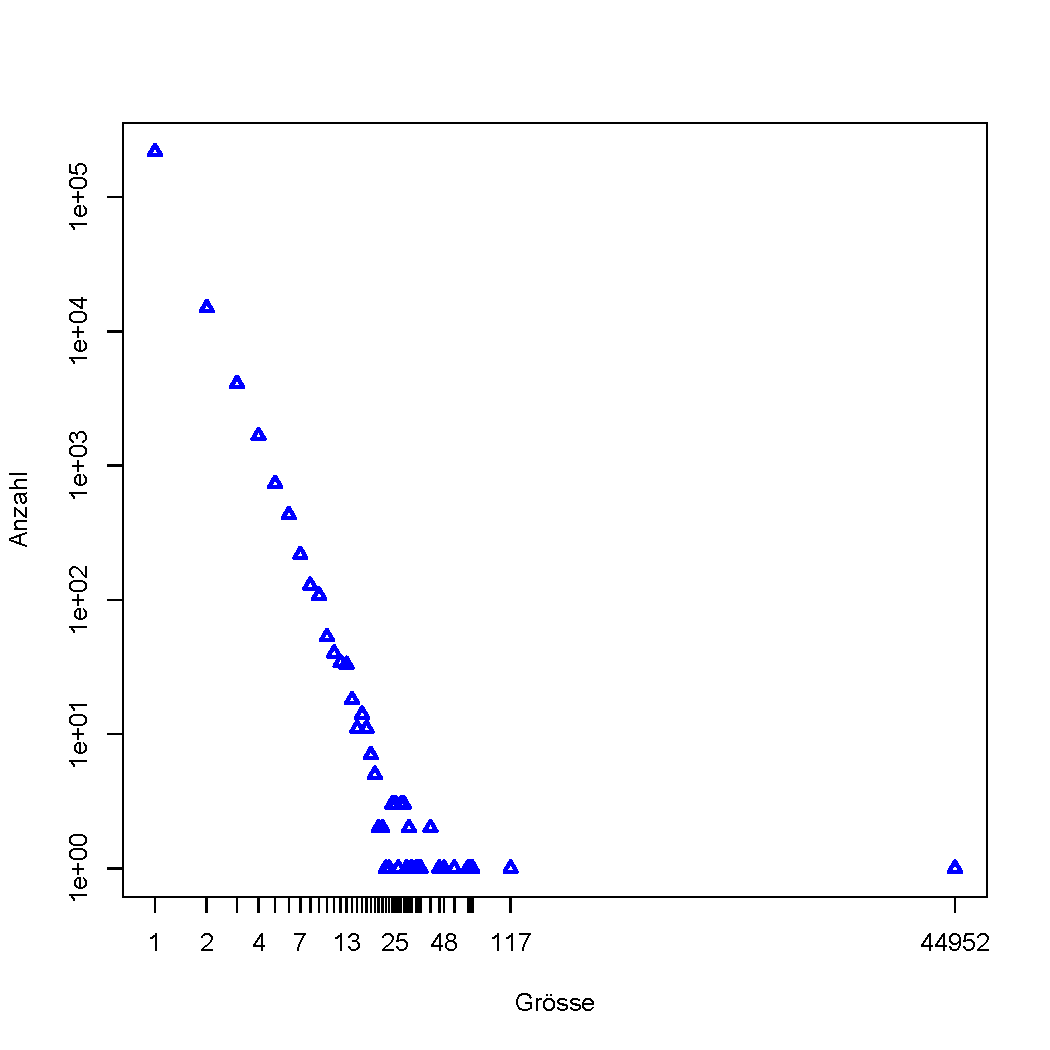
\includegraphics[scale=0.42]{images/component-size.pdf}
  \caption{Gr\"ossenverteilung der starken Zusammenhangskomponenten}
  \label{fig:component-size}
\end{figure}

Der Graph wurde zun\"achst in seine 240382 starken
Zusammenhangskomponenten zerlegt. Die Verteilung der
Komponentengr\"ossen in Abbildung \ref{fig:component-size} zeigt dabei
zwei Extreme: Es existiert eine einzelne gigantische Komponente mit
ca. 45000 Knoten. Demgegen\"uber steht eine geringe Anzahl von kleinen
Komponenten bis zur Gr\"osse 3 , insbesondere aber \"uber 100000
einelementige Komponenten, also einzelne Knoten, die nur
\emph{entweder} ein- oder ausgehende Kanten haben, und \"uber 10000
zweielementige Komponenten, also durch zwei Kanten verbundene
Knotenpaare. Ein erheblicher Anteil der \"uberhaupt vernetzten Knoten
ist also wiederum nur sehr wenig vernetzt.

\begin{figure}[th!]
  \centering
  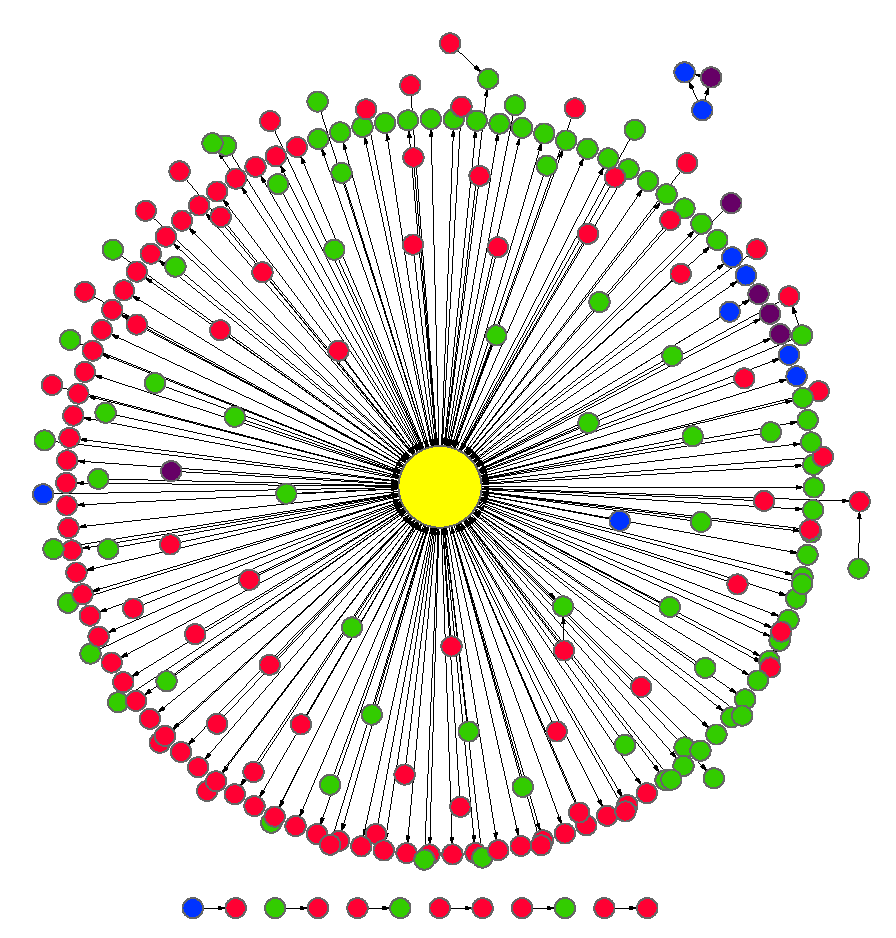
\includegraphics[scale=0.7]{images/component-metagraph-8.pdf}
  \caption{Struktur der starken Zusammenhangskomponenten bis zur
    Grösse 6 (rot = Grösse 6-10, grün = Grösse 11-20, blau = Grösse
    21-30, violett = Grösse $>= 31$, gelb = MSCC)}
  \label{fig:komponenten-struktur}
\end{figure}

Abbildung \ref{fig:komponenten-struktur} zeigt die Struktur der
Zusammenhangskomponenten bis zur Gr\"osse 6, die mit anderen
Komponenten verbunden sind. Es ergibt sich eine sternf\"ormige
Struktur, bei der die kleineren Komponenten fast ausschliesslich mit
der gr\"ossten Komponente verbunden sind und es so gut wie keine
weitere Vernetzung gibt. Um zwei starke Zusammenhangskomponenten
verschmelzen zu lassen, ist nur genau eine Kante in jede Richtung
n\"otig. Es kann also davon ausgegangen werden, dass die Komponenten
nur durch einzelne Kanten, die eben nur in eine Richtung verlaufen
k\"onnen, verbunden sind. Daraus ergibt sich, dass die Mitglieder
der kleinen Komponenten nur eine sehr geringe Signaturaktivit\"at
aufweisen k\"onnen, da andernfalls die Wahrscheinlichkeit f\"ur das Verschmelzen
von Komponenten hoch w\"are und die Anzahl sehr kleiner Komponenten
geringer sein m\"usste.

Die \emph{N\"utzlichkeit} des Web of Trust f\"ur die Teilnehmer, deren
Schl\"ussel nicht in der gr\"ossten starken Zusammenhangskomponente
enthalten sind, ist gering: Die Menge der Schl\"ussel, die von einem
Teilnehmer anhand von Signaturketten verifiziert werden kann,
beschr\"ankt sich zun\"achst auf die eigene Komponente und ist damit
sehr klein. Zwar gibt es auch -- wie oben gezeigt -- Vernetzung
zwischen kleineren Komponenten und der gr\"ossten Komponente. Es
existieren ca. 18000 Knoten, die Knoten aus der gr\"ossten Komponente
direkt \"uber eine einzige Kante errreichen k\"onnen. Allerdings muss
hier beachtet werden, dass das in PGP/GnuPG verwendete
Verifizierungsmodell die L\"ange der verwendbaren Signaturketten
begrenzt -- in der Standardeinstellung von GnuPG auf die maximale
L\"ange 5 (siehe Abschnitt
\ref{sec:das-gnupg-vertrauensmodell}). Schon innerhalb der gr\"ossten
Komponente sind viele k\"urzeste Pfade l\"anger als dieses Maximum
(siehe Abschnitt \ref{sec:kennz-des-graph}). Durch den zus\"atzlichen
Schritt zu einem Knoten innerhalb der gr\"ossten Komponente
verl\"angert sich der Pfad. Insbesondere wenn es sich bei diesen
Knoten um schwach vernetzte Knoten handelt, die am ``Rand'' der
gr\"ossten Komponente liegen, ist die Menge der auf Pfaden benutzbarer
L\"ange erreichbaren Knoten beschr\"ankt. Kann die gr\"osste
Komponente nur indirekt \"uber andere Knoten erreicht werden,
reduziert sich diese Menge noch weiter. Gleiches gilt auch f\"ur die
Erreichbarkeit der Menge von ca. 92000 Knoten, zu denen eine Kante von
Knoten der gr\"ossten Komponente aus besteht. Beachtet werden muss
allerdings die Existenz von zentralen Certificate Authorities im
eigentlich dezentralen Web of Trust. Mit den drei seit 1997 im Rahmen der
``Krypto-Kampagne'' der Zeitschrift c't (siehe Abschnitt
\ref{sec:sozi-komp-des}) verwendeten Zertifizierungsschl\"usseln
wurden insgesamt 23813 derzeit g\"ultige Schl\"ussel
unterschrieben. Von diesen liegen nur 2578 Schl\"ussel innerhalb der
gr\"ossten Komponente. Wenn also nur dem verwendeten
Zertifizierungsprozess und damit diesen drei
Zertifizierungsschl\"usseln vertraut wird, sind immerhin etwa 20000
Schl\"ussel aussserhalb der gr\"ossten Komponente verifizierbar. Es
zeigt sich hier auch die Flexibilit\"at des Web of Trust-Konzeptes,
dass die Integration von zentralen Komponenten in das eigentlich
dezentrale Netz erlaubt.

Insgesamt lassen diese Daten den Schluss zu, dass ausschliesslich die
gr\"osste starke Zusammenhangskomponente Schl\"ussel von Personen
enth\"alt, die sich durch regelm\"assige Signaturaktivit\"aten am Web
of Trust beteiligen und es zur Verifizierung von Schl\"usseln
benutzen. 

\subsection{Netzwerkstatistiken der gr\"ossten starken
  Zusammenhangskomponente}
\label{sec:kennz-des-graph}

Die weitere Untersuchung der Topologie des Graphen konzentriert sich
auf die gr\"osste starke Zusammenhangskomponente. Starke
Zusammenhangskomponenten als Einheit der Betrachtung machen Sinn, weil
die Verwendung des Graphen f\"ur die Verifizierung von Schl\"usseln
gerade die Erreichbarkeit vorraussetzt und weil eine Reihe von
Netzwerkstatistiken nur definiert sind, wenn zwischen allen Paaren von
Knoten Pfade existieren. Da im vorherigen Abschnitt argumentiert
wurde, dass die gr\"osste starke Zusammenhangskomponente die einzige
ist, die in gr\"osserem Massstab vernetzt ist und in der
Signaturaktivit\"aten stattfinden, scheint eine Untersuchung der
restlichen Komponenten nicht sinnvoll.

Der induzierte Teilgraph der gr\"ossten starken
Zusammenhangskomponente besteht aus 44952 Knoten und 442960
gerichteten Kanten. Dieser Teilgraph ist deutlich gr\"osser als die
bisher in der Literatur verwendeten PGP-Netzwerke:  ein gerichtetes
Netzwerk von ca. 12000 Knoten bei \cite{Capkun2002} und ein Netzwerk
von 10700 Knoten, bei dem alle einseitigen Signaturen gel\"oscht
wurden bei \cite{Boguna2004} und \cite{Gregory2010}. Beide Netzwerke
stellen die gr\"osste starke Zusammenhangskomponente dar und wurden im
Jahr 2001 extrahiert.

\subsubsection{Gegenseitigkeit von Kanten}
\label{sec:gegens-von-kant}

Der \emph{Reciprocity}-Wert eines gerichteten Graphen gibt den Anteil
von Kanten an, die in beide Richtungen verlaufen. F\"ur die gr\"osste
Komponente ist dieser Wert 0,510. Das bedeutet, dass es f\"ur eine
gegebene Kante eine Chance von 51\% gibt, dass eine entsprechende
``Gegenkante'' in umgekehrter Richtung existiert. Die Reciprocity
eines zuf\"alligen Graphen, der \"uber die \emph{gleiche Gradsequenz}
wie die gr\"osste Komponente verf\"ugt, hat im Vergleich eine
Reciprocity von nur 0,006. Dass der reale Wert deutlich gr\"osser ist,
ist nicht verwunderlich: Das Web of Trust ist eben kein Produkt eines
zuf\"alligen Prozesses, sondern von konkreten Mechanismen, n\"amlich
gegenseitigen Signierungen von Schl\"usseln. Eher erstaunlich ist,
dass der Wert nicht noch h\"oher ist, dass also nicht noch mehr
Signaturen auf Gegenseitigkeit beruhen. In Abschnitt
\ref{sec:sozi-komp-des} wurde dargestellt, dass die Signierung bei
Keysigning-Parties und privaten Treffen \"ublicherweise gegenseitig
verl\"auft, dass also beide Signaturpartner den Schl\"ussel des
jeweils anderen unterschreiben. Es ist eine Reihe von Gr\"unden
denkbar, die dazu f\"uhren, dass der Anteil einseitiger Signaturen so
hoch ist: Eine Rolle k\"onnten dabei Certificate Authorities
spielen. Diese signieren zwar eine Vielzahl von Schl\"usseln,
empfangen aber selbst weniger Signaturen\footnote{Beispielsweise
  verf\"ugt ein CA-Schl\"ussel, der 1684 Schl\"ussel in der gr\"ossten
  Komponente unterschrieben hat, selbst nur \"uber 683 Signaturen von
  Schl\"usseln aus dieser Komponente}. Ausserdem k\"onnen Signaturen
aus verschiedenen Gr\"unden nicht vorgenommen werden oder nicht auf
Keyserver hochgeladen werden. Schlussendlich kann nicht davon
ausgegangen werden, dass hinter jeder Signatur ein sinnvoller Prozess
der Identit\"ats\"uberpr\"ufung steht. Teilnehmer k\"onnten etwa
andere Schl\"ussel ``zum Experimentieren'' unterschreiben. PGP und
GnuPG zeigen eine Warnung an, wenn die E-Mail-Signatur eines
Schl\"ussels \"uberpr\"uft wird, der nicht als \emph{valide}
eingestuft wird. Teilnehmer k\"onnten dann versucht sein, Schl\"ussel
zu unterschreiben, deren Authentizit\"at sie nicht \"uberpr\"uft
haben, um diese Warnung zu unterdr\"ucken, selbst wenn dadurch der
Sinn des Web of Trust untergraben wird.

Abbildung \ref{fig:inoutcorr} zeigt die Verteilungsfunktion des
Verh\"altnisses von ausgehendem zu eingehendem Grad f\"ur alle Knoten
$u$ in der gr\"ossten starken Zusammenhangskomponente, also
$\frac{d^+(u)}{d^-(u)}$. Aus dieser Verteilung ergibt sich, dass eine
positive Korrelation zwischen dem eingehendem und dem ausgehendem Grad
eines Knotens besteht. F\"ur etwa die H\"alfte der Knoten (21817)
unterscheidet sich der eingehende Grad um maximal 20\% vom ausgehenden
Grad. Diese Korrelation folgt aus der hohen Anzahl gegenseitiger
Kanten und der Natur des Signaturprozesses, bei dem Schl\"ussel
\"ublicherweise gegenseitig signiert werden.

\begin{figure}[th!]
  \centering
  \subfloat[]{\label{fig:indeg-dist} 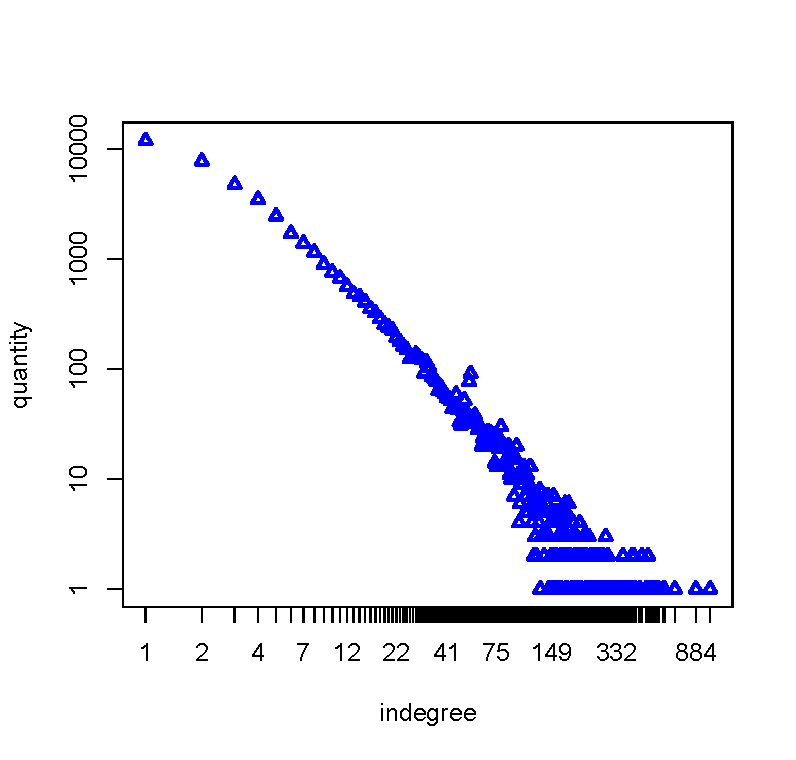
\includegraphics[scale=0.42]{images/indegree-dist.pdf}}
  \subfloat[]{\label{fig:outdeg-dist} 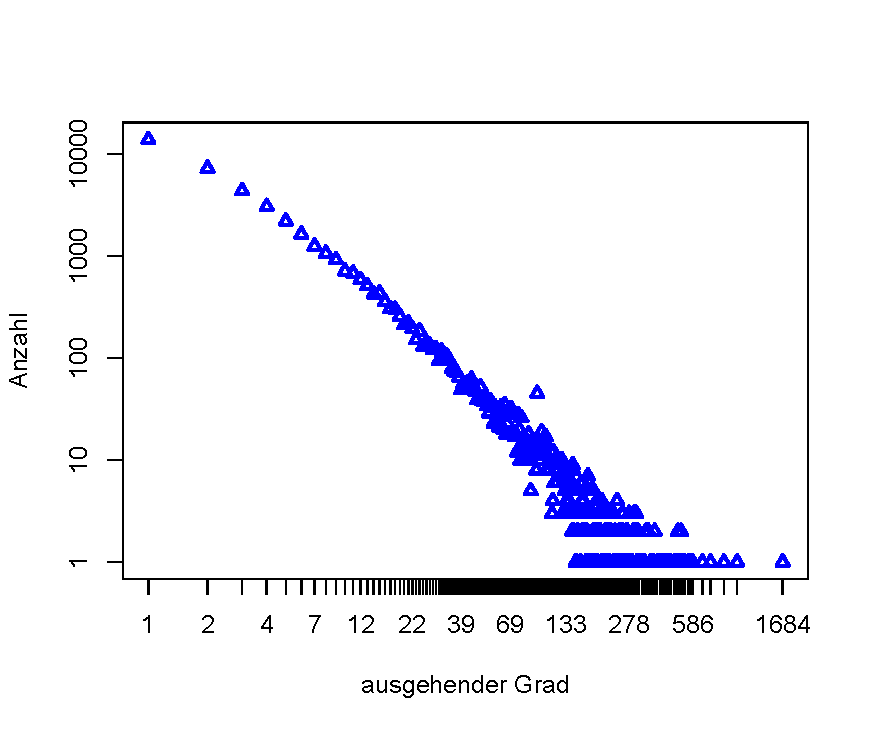
\includegraphics[scale=0.42]{images/outdegree-dist.pdf}}
  \caption{Verteilung der eingehenden \subref{fig:indeg-dist} und
    ausgehenden \subref{fig:outdeg-dist} Knotengrade in der gr\"ossten
    starken Zusammenhangskomponente}
  \label{fig:degree-dist}
\end{figure}

\subsubsection{Clustering und Small-World}
\label{sec:clustering-und-small}

F\"ur die Berechnung des Clustering-Koeffizienten wurde der eigentlich
gerichtete Graph als ungerichteter Graph betrachtet, da es keine
anerkannte Definition des Clustering-Koeffizienten f\"ur gerichtete
Graphen zu geben scheint. Diese Vorgehensweise scheint die in der
Literatur \"ubliche zu sein. Selbstverst\"andlich ist anzunehmen, dass
das Ergebnis verf\"alscht wird, wenn gerichtete Kanten als
ungerichtete Kanten betrachtet werden. Allerdings wurde bereits
gezeigt, dass ein erheblicher Anteil der Kanten symmetrisch ist, also
in beide Richtungen verl\"auft, und eine positive Korrelation zwischen
dem ausgehendem und dem eingehenden Grad von Knoten besteht. Der
Schaden sollte sich also in Grenzen halten.

Der durchschnittliche Clustering-Koeffizient f\"ur die MSCC betr\"agt
$C = 0,460$. Das bedeutet, dass \emph{im Durchschnitt} etwa die
H\"alfte der Nachbarn eines Knoten wieder verbunden sind. Der Graph
zeigt also ein erhebliches Mass an Clustering. Zum Vergleich betr\"agt
der Clustering-Koeffizient f\"ur ein \emph{zuf\"alliges} Netzwerk mit
der gleichen Anzahl von Knoten und Kanten $C = 0,00025$ und f\"ur ein
zuf\"alliges Netzwerk, dass ausserdem \"uber die gleiche Sequenz von
Graden verf\"ugt, $C = 0,013$. In der MSCC findet sich also wesentlich
mehr Clustering, als in einem zuf\"allig entstandenen Netzwerk zu
erwarten w\"are.

Newman und Park bemerken, dass ein hohes Mass an Clustering
charakteristisch f\"ur soziale Netzwerke ist und sie von vielen
nicht-sozialen Netzwerken unterscheidet\cite{PhysRevE.68.036122}. Als
m\"oglichen Grund geben sie an, dass sich die Knoten in sozialen
Netzwerken \"ublicherweise in \emph{Communities} einteilen lassen,
also Gruppen von Knoten, die untereinander st\"arker vernetzt sind als
nach aussen. Intuitiv ist naheliegend, dass in einer solchen Community
die Wahrscheinlichkeit, dass zwei Nachbarn eines Knoten durch eine
Kante verbunden sind, hoch ist. In Abschnitt
\ref{sec:result-zusamm-und-comm} wird gezeigt, dass der vorliegende
Graph in der Tat \"uber eine markante Community-Struktur verf\"ugt.

Der Durchschnitt aller Distanzen in der gr\"ossten starken
Zusammenhangskomponente betr\"agt 12,14 (siehe auch Abbildung
\ref{fig:avg-pathlen} f\"ur die Verteilung der durchschnittlichen
Distanzen pro Knoten). Dieser Wert ist in Relation zur Anzahl der
Knoten im Netzwerk gering und zeigt, dass der Graph den
``Small-World''-Effekt aufweist, dass also jedes Paar von Knoten mit
hoher Wahrscheinlichkeit durch einen Pfad von geringer L\"ange
verbunden ist. Dieser Effekt tritt in vielen untersuchten Netzwerken
auf und ist insbesondere typisch f\"ur soziale Netzwerke
\cite{newman:167}.

Interessant ist die geringe Distanz auch, weil die Teilnehmer des Web
of Trust aus verschiedensten L\"andern und damit aus verschiedensten
geographischen Regionen stammen. Die \"ubliche Prozedur f\"ur das
Signieren von Schl\"usseln setzt ein direktes, d.h. r\"aumliches
Treffen der teilnehmenden Personen vorraus. Eine Interpretation der
geringen Distanz w\"are, dass eine Anzahl von Teilnehmern geographisch
so mobil ist, dass sich Signierungen an weit auseinanderliegenden
Orten ergeben, die f\"ur die Verbindungen zwischen geographisch
eigentlich weit entfernten Bereichen im Netzwerk sorgen. Allerdings
wurde hier nur der Durchschnitt der Distanzen betrachtet. Es kann
nicht ausgeschlossen werden, dass sich der niedrige Durchschnitt f\"ur
die einzelnen Knoten nur ergibt, weil die Knoten aus dem eigenen Land
bzw. der eigenen geographischen Region auch im Netzwerk sehr nahe
liegen. In Abschnitt \ref{sec:result-zusamm-und-comm} wird gezeigt,
dass sich die meisten Communities anhand von Top-Level-Domains einem
Land oder Sprachraum zuordnen lassen. Interessant w\"are an dieser
Stelle eine Untersuchung, inwiefern sich die geographische Distanz der
L\"ander auch in der Distanz im Netzwerk der entsprechenden
Communities wiederspiegelt.
\subsubsection{Verteilung der Grade, Skalenfreiheit}
\label{sec:verteilung-der-grade}

Der durchschnittliche ausgehende Grad (und damit auch der
durchschnittliche eingehende Grad) betr\"agt 9,29. Allerdings zeigen
Abbildung \ref{fig:indeg-dist} und \ref{fig:outdeg-dist}, dass dieser
Durchschnitt auf h\"ochst ungleichm\"assige Weise zustande
kommt. W\"ahrend eine Mehrheit der Knoten einen sehr kleinen ein-
bzw. ausgehenden Grad hat, existiert eine signifikante Anzahl von
Knoten, deren Grad deutlich \"uber dem Durchschnitt liegt. Dieses
Verhalten ist konsistent mit einer Power-Law-Verteilung der Grade und
die in etwa geraden Linien im doppelt logarithmischen Plot der
Verteilungen legen dies zus\"atzlich nahe. Allerdings wird in
\cite{Clauset2009} argumentiert, dass ein ``Nachweis'' einer
Power-Law-Verteilung und insbesondere die Berechnung des
Power-Law-Koeffizienten etwa mit linearer Regression auf einem doppelt
logarithmischen Plot (vorgeschlagen etwa bei \cite{Brinkmeier2004}) zu
stark verf\"alschten Ergebnissen f\"uhren kann. Stattdessen wird hier
die von Clauset et al. vorgeschlagene Vorgehensweise benutzt, die
beste Power-Law-Anpassung mittels der Maximum-Likelihood-Methode zu
berechnen. Damit ergibt sich f\"ur die Verteilung der ein-
bzw. ausgehenden Grade ein Power-Law-Koeffizient von XX bzw. XY. Diese
Werte liegen im \"ublichen Rahmen f\"ur Netzwerke, die aus sozialen
Interaktionen entstehen (FIXME: cite). Allerdings ergibt die
\"Uberpr\"ufung der Qualit\"at der Anpassung mittels des
Kolmogorov-Smirnov-Tests Werte, die mit $p = 0,012$ und $p = 0,011$
deutlich unter dem in \cite{Clauset2009} empfohlenen Schwellwert von
$p=0,1$ liegen und damit ein Power-Law als plausible Hypothese f\"ur
die Verteilung ausschliessen.

\begin{figure}[th!]
  \centering
  \subfloat[]{\label{fig:inoutcorr} 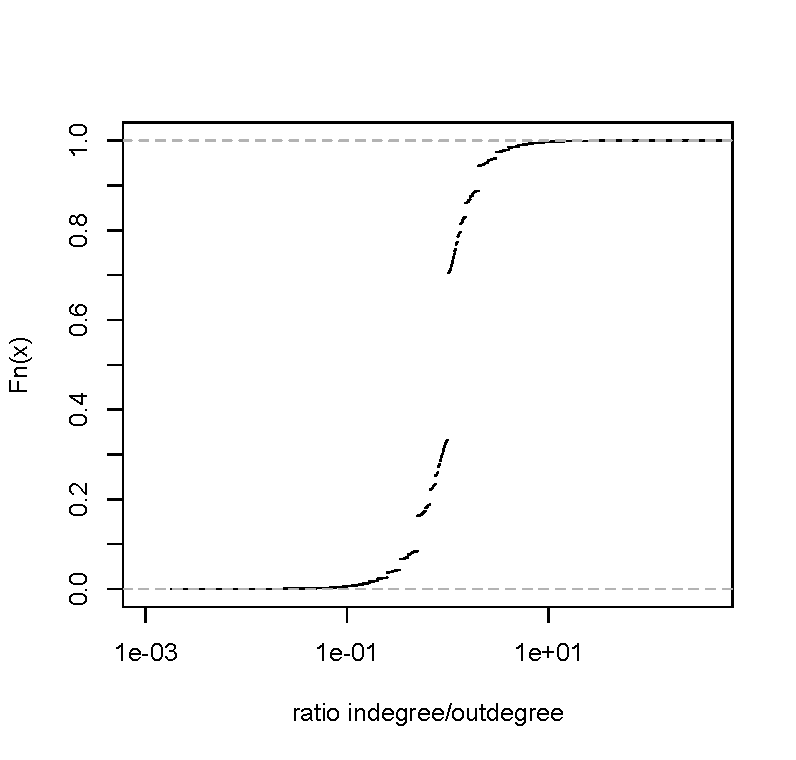
\includegraphics[scale=0.55]{images/inoutcorr.pdf}}
  \subfloat[]{\label{fig:knn} 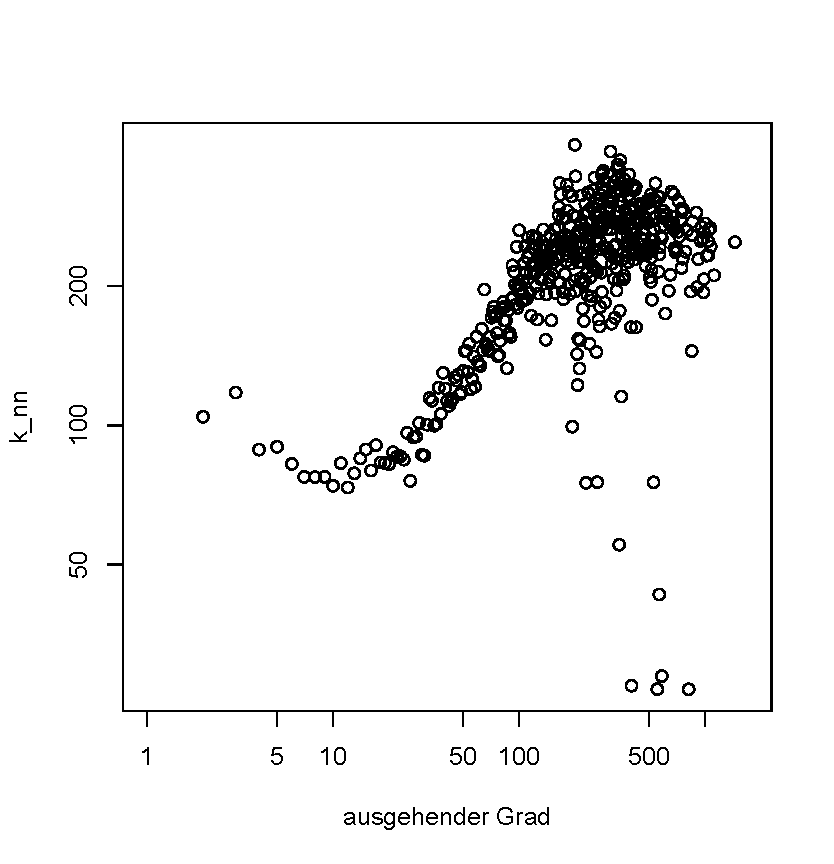
\includegraphics[scale=0.55]{images/knn.pdf}}
  \caption{Kumulative Verteilungsfunktion von $\frac{d^+(u)}{d^-(u)}$
    f\"ur alle Knoten $u$ in der MSCC
    \subref{fig:inoutcorr}. Verteilung von $k_{nn}$ \"uber alle
    ausgehenden Grade \subref{fig:knn}.}
  \label{fig:degree-correlation}
\end{figure}

Es handelt sich bei dem vorliegenden Netzwerk also nicht um ein
skalenfreies Netzwerk im engeren Sinne. Es stellt sich allerdings die
Frage, ob das \"uberhaupt relevant ist. Zum einen zeigt die Verteilung
der Grade Merkmale, die mit charakteristischen Merkmalen einer
Power-Law-Verteilung \"ubereinstimmen, n\"amlich die hohe
Variabilit\"at der Grade und insbesondere die Anwesenheit einer
signifikaten Anzahl von Knoten mit hohem Grad. Die Verteilung
\emph{\"ahnelt} also immerhin einer Power-Law-Verteilung. Eine
zentrale Rolle bei den Eigenschaften, die skalenfreien Netzwerken
zugeschrieben werden, spielt die Existenz eines Kerns bestehend aus
``Hubs'', also Knoten mit hohem Grad, die untereinander verbunden
sind. Knoten mit niedrigem Grad sind prim\"ar mit diesen Hubs
verbunden. Dieser Kern h\"alt das Netzwerk zusammen und sorgt f\"ur
geringe Distanzen. Allerdings haben Li et al. \cite{Li2005} gezeigt,
dass die Existenz einer Power-Law-Verteilung nicht ausreicht, um die
Existenz von Hubs nachzuweisen. Es existieren Netzwerke, die zwar eine
Power-Law-Verteilung der Grade haben, bei denen die Knoten mit hohem
Grad aber eher an der \emph{Peripherie} liegen und keine zentrale
Rolle im Sinne von Hubs \"ubernehmen.  Hubs ergeben sich erst dann,
wenn Knoten mit hohem Grad prim\"ar mit Knoten vernetzt sind, die
wiederum einen hohen Grad haben. Im Umkehrschluss kann angenommen
werden, dass ein Netzwerk, welches in charakteristischen Aspekten
einem skalenfreien Netzwerk \emph{\"ahnelt}, auch \"ahnliche
Eigenschaften aufweisen \emph{kann}.

Um zu \"uberpr\"ufen, ob die gut vernetzten Knoten als Hubs fungieren,
wurde zun\"achst die Korrelationsfunktion $k_{nn}$
berechnet\cite{PhysRevLett.87.258701}. Diese verbindet f\"ur
gerichtete Graphen einen Grad $d$ mit dem Durchschnitt des Grads der
Nachbarn der Knoten, die diesen Grad $d$ haben. Sie misst also, wie
hoch der Grad von Knoten ist, die mit Knoten vom Grad $d$ verbunden
sind. Abbildung \ref{fig:knn} zeigt die Verteilung von $k_{nn}$ \"uber
alle Grade $d$. Aus der ansteigenden Kurve f\"ur ansteigende Grade
kann geschlossen werden, dass Knoten mit hohem Grad dazu tendieren, zu
anderen Knoten mit hohem Grad verbunden zu sein. Diese Knoten scheinen
also in der Tat einen \emph{Kern} des Netzwerkes zu bilden. Um dies zu
untermauern, wurde zus\"atzlich noch der Assortativity-Koeffizient $r$ \cite{PhysRevLett.89.208701}
berechnet, welcher zwischen -1 und 1 liegt. Ein positiver Wert von $r$
bedeutet, dass eine positive Korrelation zwischen den Graden der
Knoten besteht. Im gegens\"atzlichen Fall einer negativen Korrelation
ist $r$ negativ. Es ergibt sich ein Wert $r = 0,113$. Aus diesem positiven
Wert folgt also ebenfalls, dass Knoten tendenziell mit Knoten verbunden
sind, die einen \"ahnlichen Grad haben. Der $r$-Wert \"ahnelt den
Werten, die f\"ur andere soziale Netzwerke berechnet
wurden\cite{newman:167}.

Zwar scheint die in \cite{Li2005} definierte $s$-Metrik ein besser
geeignetes Mass f\"ur die Charakterisierung der Korrelation von Graden
benachbarter Knoten zu sein als der Assortativity-Koeffizient
$r$. Diese wurde hier aber nicht verwendet, da die Implementierung des
Algorithmus f\"ur die Berechung des Normalisierungswertes $s_{max}$ zu
aufw\"andig war.

\subsection{Robustheit}
\label{sec:robustheit}

\begin{figure}[ht!]
  \centering
  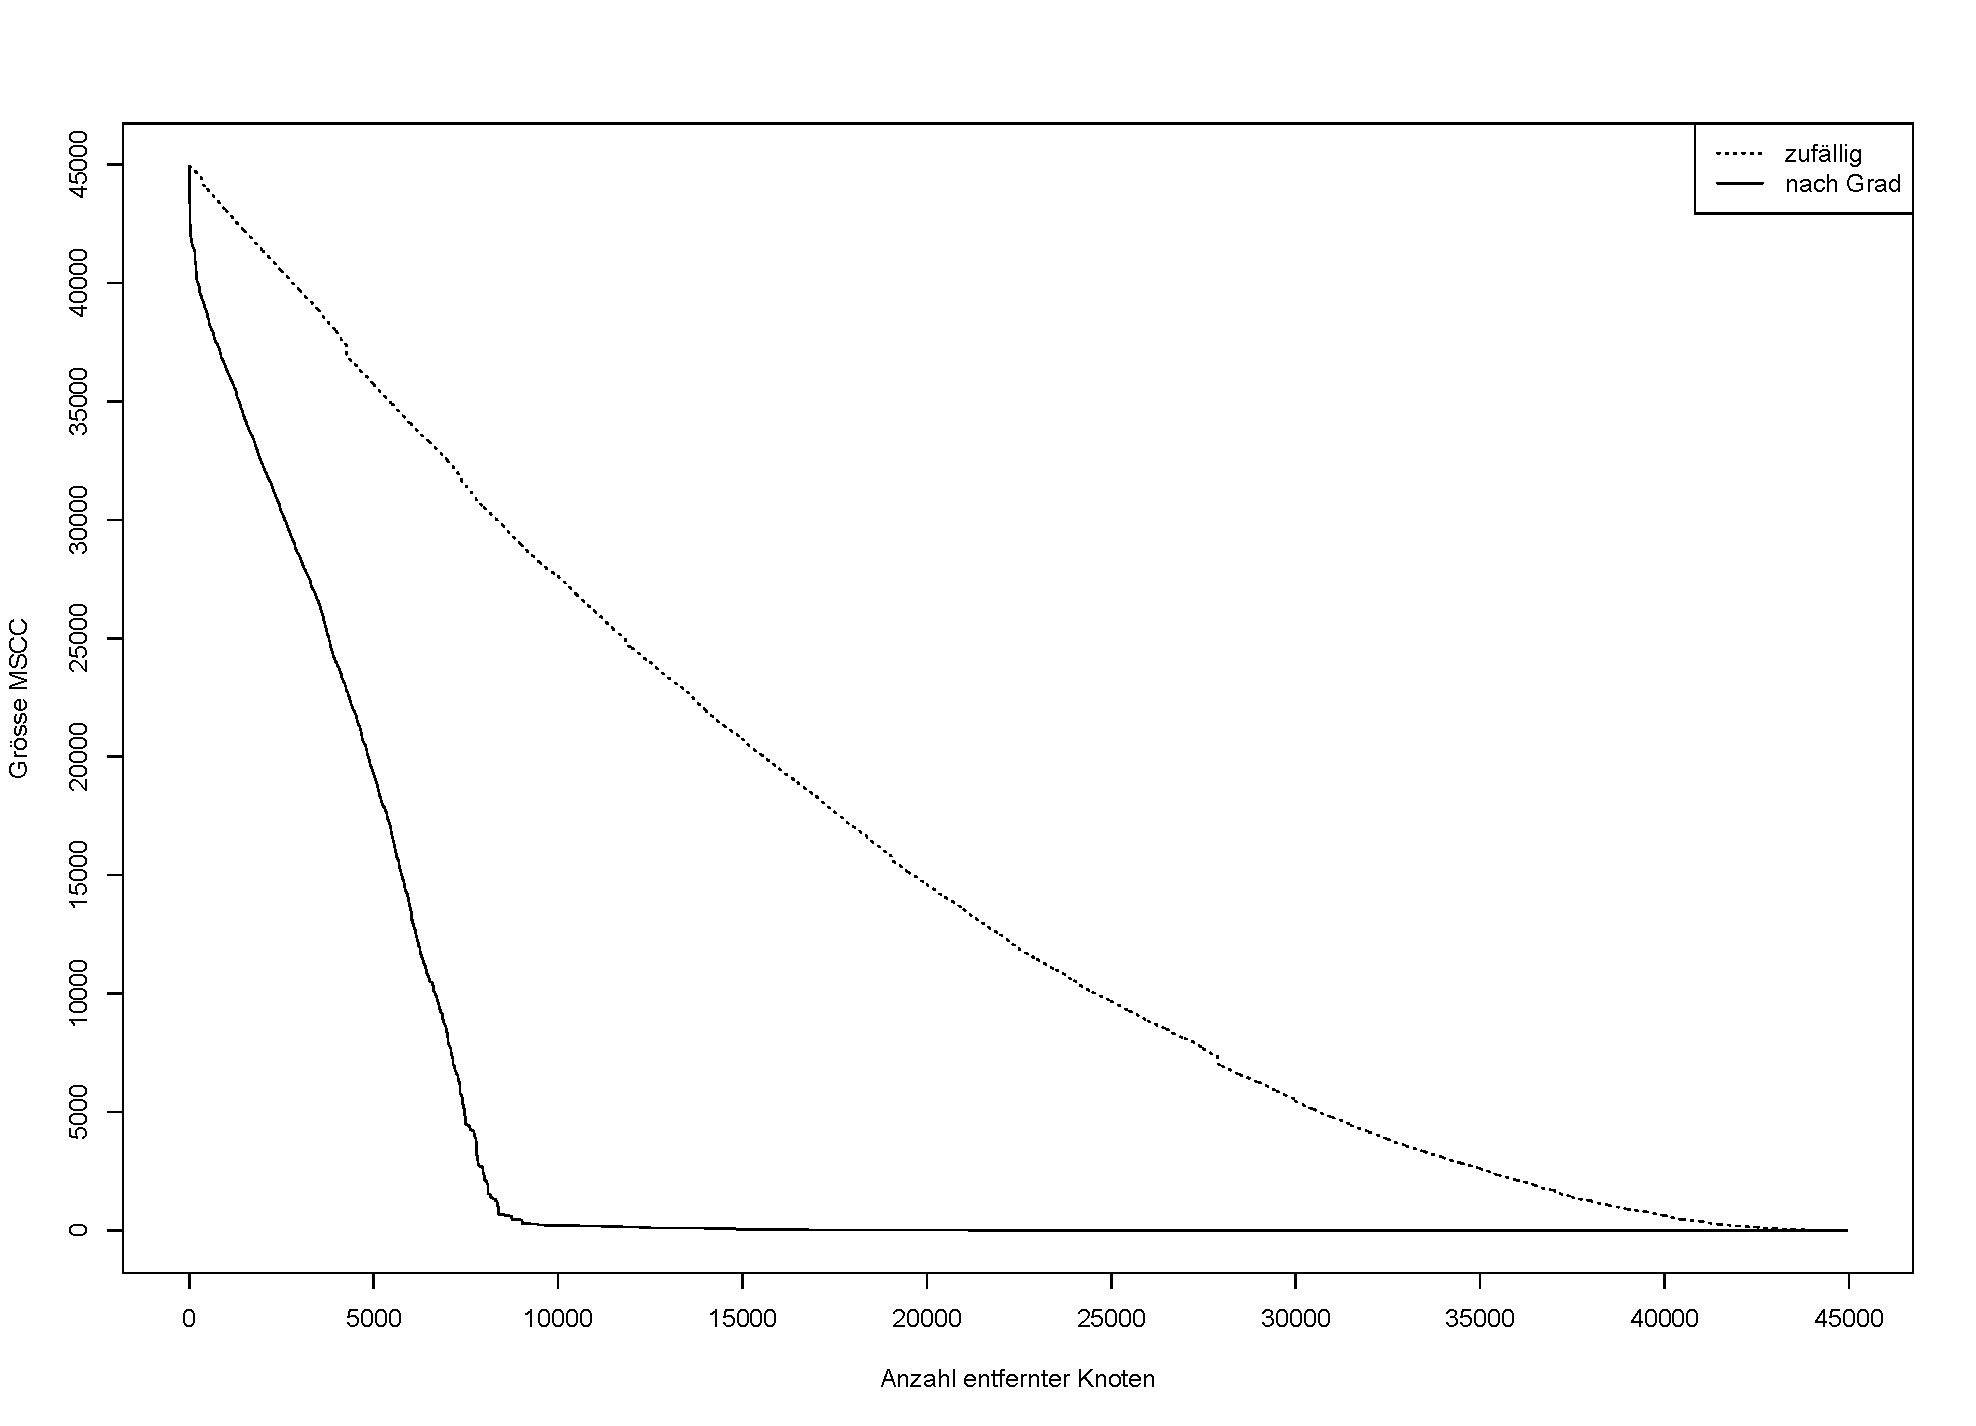
\includegraphics[scale=0.45]{images/without.pdf}
  \caption{Entwicklung der Gr\"osse der gr\"ossten starken
    Zusammenhangskomponente, wenn Knoten zuf\"allig oder nach absteigender
    Gr\"osse entfernt werden}
  \label{fig:without}
\end{figure}

In diesem Zusammenhang stellt sich auch die Frage nach der
\emph{Robustheit} des Netzwerkes.  Eine Eigenschaft, die skalenfreien
Netzwerken \"ublicherweise zugeschrieben wird\cite{Albert2000}, ist
eine typische Reaktion auf das Entfernen von Knoten: W\"ahrend die
Entfernung zuf\"allig ausgew\"ahlter Knoten kaum Schaden anrichtet,
reagiert das Netzwerk sehr verwundbar auf die Entfernung von Knoten,
die sehr gut vernetzt sind. Schon die Entfernung weniger sehr gut
vernetzter Knoten f\"uhrt dazu, dass das Netzwerk zerf\"allt.

Dieser Unterschied kann aufgefasst werden als der Unterschied zwischen
einem gerichteten \emph{Angriff} und einer zuf\"alligen
\emph{Sch\"adigung}. Ein Angreifer mit der Intention, das Netz an sich
zu sch\"adigen, wird solche Knoten ausw\"ahlen, deren Entfernung einen
m\"oglichst grossen Effekt hat. Demgegen\"uber kann angenommen werden,
dass die Wahrscheinlichkeit einer zuf\"alligen Sch\"adigung in etwa
gleichverteilt \"uber alle Schl\"ussel ist. Ein Angreifer k\"onnte
beispielsweise versuchen, Knoten zu entfernen, indem er den
Schl\"ussel an sich kompromittiert oder den Zugriff auf das
Schl\"usselmaterial unm\"oglich macht, so dass der Schl\"ussel
widerrufen werden muss. Demgegen\"uber k\"onnen Schl\"ussel auf
``normalem'' Wege aus dem Netz verschwinden, wenn sie ablaufen oder
beispielsweise aufgrund des Verlusts der Passphrase widerrufen werden
m\"ussen.

Eine offensichtliche Metrik f\"ur die Wichtigkeit eines Knotens und
damit eine Strategie f\"ur die Auswahl des Zielknotens ist der
Knotengrad. Je h\"oher der Grad eines Knotens, desto wichtiger ist er
potentiell f\"ur das Netzwerk. Um die Robustheit unter dieser
Auswahlstrategie zu testen, wurden aus der gr\"ossten starken
Zusammenhangskomponente sukzessive Knoten in der Reihenfolge
absteigender ausgehender Grade bzw. in einer zuf\"alligen Reihenfolge
entfernt. Abbildung \ref{fig:without} zeigt die Entwicklung der
Gr\"osse der gr\"ossten Komponente, wenn mehr und mehr Knoten entfernt
werden. Bei der Entfernung zuf\"allig ausgew\"ahlter Knoten ist das
Netzwerk ausgesprochen stabil. Die gr\"osste Komponente schrumpft fast
im gleichen Masse, wie Knoten entfernt werden. Dieses Ergebnis ist
nicht \"uberraschend. Da ein hoher Anteil der Knoten einen sehr
niedrigen Grad hat, ist bei zuf\"alliger Auswahl die Chance, einen
solchen Knoten zu treffen, hoch. Das Verschwinden von Schl\"usseln
durch Ablaufen ist ein normaler und h\"aufiger Prozess. So verf\"ugen
etwa 5700 Schl\"ussel in der gr\"ossten starken
Zusammenhangskomponente \"uber ein Ablaufdatum, werden also irgendwann
aus dem Netz verschwinden. Dieser Fall richtet also kaum globalen
Schaden im Netzwerk an.

Der Schaden durch die Entfernung von Knoten mit hohem ausgehendem Grad
ist deutlich gr\"osser. Hier f\"uhrt schon die Entfernung von deutlich
weniger Knoten zu einem raschen Verfall bis hin zur v\"olligen
Aufl\"osung des Netzwerkes. Aber auch hier richtet die Entfernung
\emph{einzelner} Knoten noch keinen signifikanten Schaden an. Erst ab
etwa 100 Knoten -- was der Entfernung aller Knoten mit einem
ausgehenden Grad gr\"osser 250 entspricht -- sinkt die Gr\"osse der
Komponent erheblich. Die M\"oglichkeiten eines Angreifers d\"urften
sich eher im Entfernen einzelner Knoten ersch\"opfen, so dass der zu
erwartende Schaden gering ist. Trotzdem ist die Abh\"angigkeit des
Netzwerks von wenigen Knoten bemerkenswert. Der rasche Verfall bei der
Entfernung dieser Knoten illustriert die Wichtigkeit dieser zentralen
Knoten, die als ``Hubs'' das Netzwerk zusammenhalten.

Dieses Verhalten ist konsistent mit dem Verhalten, dass viele --
insbesondere soziale -- Netzwerke aus der realen Welt zeigen, die als
skalenfrei eingeordnet werden FIXME cite. 

Angemerkt werden muss, dass neben der Gr\"osse der Komponente auch
eine Betrachtung der Entwicklung der Distanzen in der Komponente
sinnvoll w\"are. Dass die Komponentengr\"osse sich im Fall
zuf\"alliger Reihenfolge stabil verh\"alt, muss nicht bedeuten, dass
sich die durchschnittlichen Distanzen nicht deutlich
vergr\"ossern. Vergr\"ossern sich die Distanzen und verl\"angern sich
damit die n\"otigen Signaturketten, so sinkt die N\"utzlichkeit des
Netzwerkes (siehe Abschnitt \ref{sec:nutzlichkeit}). F\"ur die
Entfernung von Knoten anhand des Grades wird aufgrund der
\"Ahnlichkeit zu skalenfreien Netzwerken erwartet, dass sich die
Distanzen schon durch die Entfernung weniger Knoten merklich
erh\"ohen. Aufgrund des notwendigen Rechenaufwandes konnte dies im
Rahmen dieser Arbeit aber nicht durchgef\"uhrt werden.

Der Grad eines Knoten ist nicht unbedingt das geeignetste Mass f\"ur
die globale ``Wichtigkeit'' des Knotens. Durch eine Konzentration auf
\emph{zentrale} Knoten, also etwa solche mit einer hohen Betweeness
Centrality, l\"asst sich m\"oglicherweise mehr Schaden anrichten. Dies
l\"asst sich am Beispiel von Certificate Authorities im Web of Trust
illustrieren: CA-Schl\"ussel haben zwar \"ublicherweise einen hohen
ausgehenden Grad, haben also viele Schl\"ussel signiert und damit
relativ kurze Wege zu vielen Schl\"usseln. Allerdings haben sie
gleichzeitig einen niedrigen eingehenden Grad, weil ein CA-Schl\"ussel
\"ublicherweise nicht mit einer Person direkt verbunden ist, und damit
das \"ubliche Verifizieren der Identit\"at wenig Sinn macht. Damit
tauchen CA-Schl\"ussel nur auf relativ wenigen k\"urzesten Pfaden auf,
da sie selbst eher schlecht erreichbar sind. Ihre Entfernung richtet
also -- zumindest in Bezug auf die Distanzen -- einen relativ geringen
Schaden an.

\subsection{N\"utzlichkeit}
\label{sec:nutzlichkeit}
Die gr\"osste Komponente enth\"alt eine erhebliche Anzahl von Knoten
mit einem ausgehenden Knotengrad von 1. Ein solch niedriger Grad
stellt eine erhebliche Einschr\"ankung f\"ur die Benutzbarkeit dieses
Schl\"ussels f\"ur die Verifizierung von anderen Schl\"usseln dar. Da
ein Schl\"ussel $A$ mit ausgehendem Grad 1 nur einen Schl\"ussel $B$
signiert hat, gibt es auch nur genau einen Schl\"ussel, \"uber den
eine Signaturkette aufgebaut werden kann. Nat\"urlich wird dadurch die
Menge insgesamt erreihbarer Knoten stark eingeschr\"ankt. Ausserdem
aber existiert damit keine Redundanz. Der Besitzer des Schl\"ussels
$A$ muss dem Besitzer des Schl\"ussels $B$ vertrauen, wenn er irgend
eine Signaturkette benutzen will. $B$ stellt einen \emph{Single point
  of failure} dar, da $A$ vom Netz getrennt wird, wenn $B$ etwa
abl\"auft oder zur\"uckgezogen wird. \"Aquivalent ist die
Verifizierbarkeit eines Knotens $A$ stark eingeschr\"ankt, wenn er
einen eingehenden Grad von 1 hat und nur von einem einzigen
Schl\"ussel $B$ signiert wurde. F\"ur die Verifizierung von $A$ muss
zwingend dem Besitzer von $B$ vertraut werden. Ist $B$ nicht mehr
benutzbar, wird $A$ vom Netz getrennt.

Klar ist, dass in einer starken Zusammenhangskomponente jeder Knoten
jeden anderen Knoten erreichen kann. Eine Mindestvorraussetzung f\"ur
die Verifizierung eines Schl\"ussels ist, dass eine Signaturkette zu
diesem Schl\"ussel aufgebaut werden kann, dass also der Knoten im
Graph erreicht werden kann. Allerdings ist die Erreichbarkeit an sich
hier nicht von Bedeutung. Vielmehr muss die Erreichbarkeit unter den
Beschr\"ankungen des PGP/GnuPG-Vertrauensmodells (siehe Abschnitt
\ref{sec:das-gnupg-vertrauensmodell}) betrachtet werden. Hier gilt
insbesondere die Einschr\"ankung, dass Signaturketten maximal die
L\"ange 5 haben d\"urfen. Es stellt sich hier die Frage nach der
N\"utzlichkeit des Netzwerkes f\"ur dessen eigentlichen Zweck, die
Verifizierung von Schl\"usseln. Diese ist dann hoch, wenn f\"ur viele
Knoten eine hohe Zahl von Knoten verifizierbar
ist. Selbstverst\"andlich bedeutet das Vorhandensein einer
Signaturkette von hinreichend geringer L\"ange noch nicht, dass ein
Schl\"ussel tats\"achlich verifizierbar ist. Zus\"atzlich muss noch
jedem Glied dieser Kette \emph{vertraut} werden. Wird Personen nur
\emph{geringf\"ugig} vertraut, sind zus\"atzlich noch weitere
redundante Signaturen n\"otig. Da diese Vertrauensinformationen aber
nicht \"offentlich verf\"ugbar sind, wird hier als obere Grenze f\"ur
die Anzahl verifizierbarer Schl\"ussel nur die maximale Pfadl\"ange
verwendet.

\begin{figure}[th!]
  \centering
  \subfloat[]{\label{fig:avg-pathlen}\includegraphics[scale=0.3]{images/pathlen-dist.pdf}}
  \subfloat[]{\label{fig:eccentricity}\includegraphics[scale=0.3]{images/ecc-dist.pdf}}
  \caption{Verteilung der (gerundeten) durchschnittlichen Distanzen 
    \subref{fig:avg-pathlen} und der Eccentricity
    \subref{fig:eccentricity} in der gr\"ossten starken Zusammenhangskomponente}
  \label{fig:pathlen-dist}
\end{figure}

Aus Abbildung \ref{fig:eccentricity} ist ersichtlich, dass die
Eccentricity, also die \emph{maximale} Distanz eines Knotens zu
irgendeinem anderen Knoten, zwischen dem Minumum 16 (dem \emph{Radius}
des Graphen) und dem Maximum 36 (dem \emph{Durchmesser} des Graphen)
liegt. F\"ur die meisten Knoten liegt sie bei 26 bis 31. Damit wird
die maximale Pfadl\"ange deutlich \"uberschritten. F\"ur alle Knoten
gilt also, dass die am weitesten entfernten Knoten grunds\"atzlich
nicht erreichbar sind. Aber auch schon die \emph{durchschnittliche}
Distanz (Abbildung \ref{fig:pathlen-dist}) ist f\"ur eine erhebliche
Anzahl von Knoten gr\"osser als die maximal erlaubte L\"ange. Klar ist
also, dass f\"ur die Mehrzahl der Knoten l\"angst nicht alle Knoten
unter der Beschr\"ankung der Pfadl\"ange erreichbar sind.

Die Gr\"osse der 5-Nachbarschaft eines Knotens gibt die Anzahl der
Knoten an, die unter dieser Beschr\"ankung erreichbar sind. Allerdings
macht es Sinn, nicht nur die 5-Nachbarschaft, sondern auch die
$n$-Nachbarschaften f\"ur $n=2,\dots,4$, also k\"urzere
Signaturketten, zu betrachten. Da jedem einzelnen Glied einer
Signaturkette vertraut werden muss, steigt mit der L\"ange der Kette
auch die Wahrscheinlichkeit, dass dieses Vertrauen eben nicht in alle
Glieder vorhanden ist. Da das Web of Trust ein soziales Netzwerk
darstellt, kann angenommen werden, dass im Allgemeinen mit der
Entfernung zu einem Knoten im Graph auch die soziale und geographische
Entfernung zu der entsprechenden Person steigt. Damit sinkt auch die
Wahrscheinlichkeit, dass weiter entfernten Personen aufgrund von
pers\"onlicher Bekanntschaft vertraut werden kann. Dass einer Person,
deren Schl\"ussel selbst signiert wurde, vertraut wird, ist
wahrscheinlicher als dass einer Person vertraut wird, deren
Schl\"ussel nicht selbst signiert wurde. Je l\"anger also
eine Signaturkette, desto niedriger die Chance, dass sie tats\"achlich
benutzbar ist. 

\begin{figure}[th!]
  \centering
  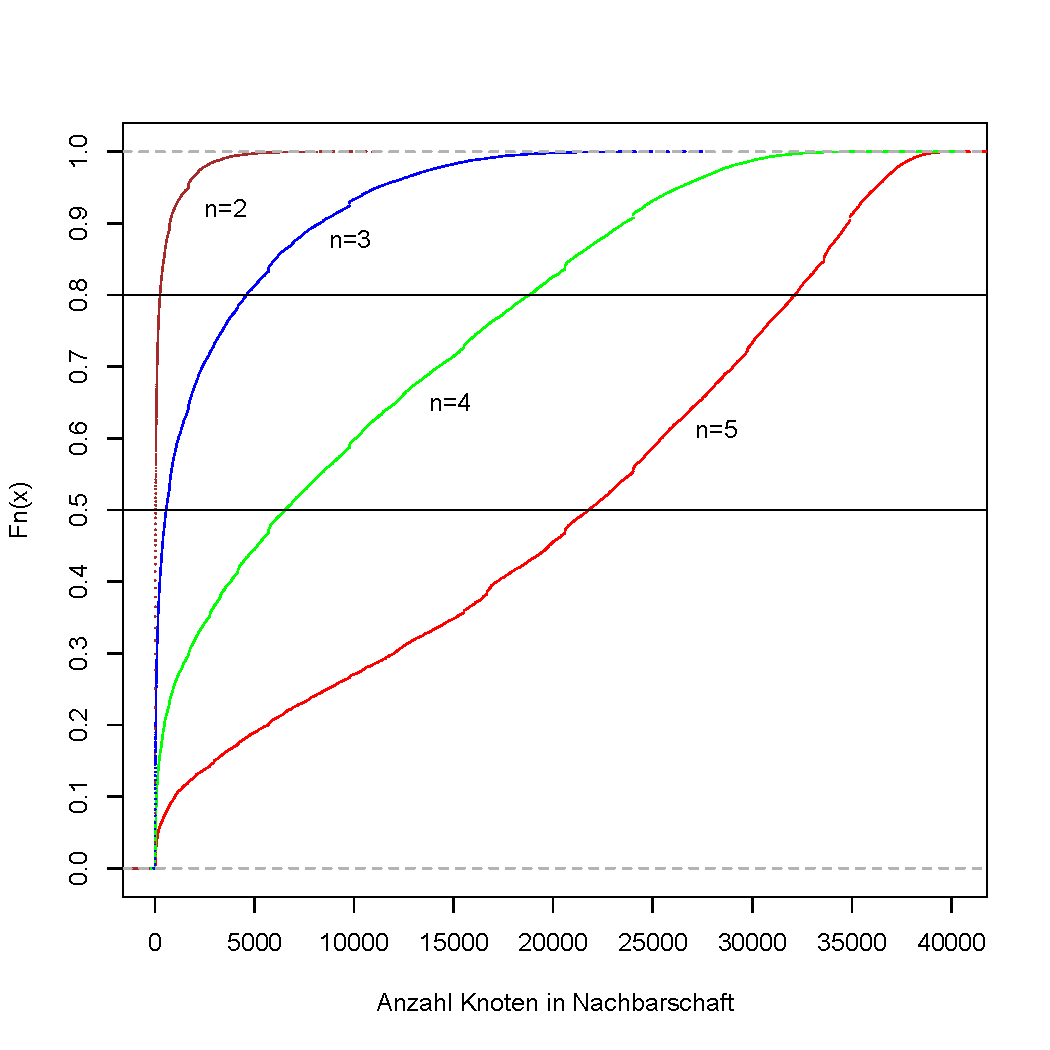
\includegraphics[scale=0.6]{images/neighbourhood-cdf.pdf}
  \caption{Kumulative Verteilungsfunktion der Nachbarschaftsgr\"ossen
    in der gr\"ossten starken Zusammenhangskomponente}
  \label{fig:neighbourhood-cdf}
\end{figure}

Abbildung \ref{fig:neighbourhood-cdf} zeigt die kumulative
Verteilungsfunktion der Gr\"osse dieser Nachbarschaften. Auff\"allig
ist hier zun\"achst das steile Wachstum der Kurve f\"ur die
2-Nachbarschaft, woraus geschlossen werden kann, dass diese
Nachbarschaft f\"ur fast alle Knoten sehr klein ist. In der Tat liegt
das 2. Quantil bei 30 und das 3. Quantil bei 160. F\"ur die Mehrzahl
der Schl\"ussel ist also die Menge der Schl\"ussel, f\"ur deren
Verifizierung nur einer Person voll vertraut werden muss, sehr
gering. Immerhin steigt die Gr\"osse der Nachbarschaften mit
wachsender Distanz deutlich: F\"ur $n=3$ liegt das 3. Quantil bereits
bei 3371. F\"ur $n=4$ und $n=5$ betr\"agt es 16340 bzw. 30530. Mittels
l\"angerer Signaturketten kann also die Mehrzahl der Teilnehmer einen
signifikanten Anteil der in der gr\"ossten Zusammenhangskomponente
vorhandenen Schl\"ussel \emph{potentiell}
erreichen. Interessanterweise liegt das Maximum der
Nachbarschaftsgr\"ossen f\"ur $n=5$ bei nur 40180. Nicht einmal f\"ur
die am besten vernetzten Schl\"ussel sind also alle Schl\"ussel mit
beschr\"ankter Kettenl\"ange erreichbar.

Wie bereits erw\"ahnt, enth\"alt die gr\"osste Zusammenhangskomponente
die Schl\"ussel mehrerer zentraler Certificate
Authorities. Interessant ist eine Absch\"atzung, wie sehr das
eigentlich dezentrale Web of Trust auf diese zentralen Komponenten
aufbaut. Um dies festzustellen wurden die Schl\"ussel der gr\"osseren
Certificate Authorities (siehe Abschnitt \ref{sec:sozi-komp-des}) aus
der gr\"ossten Komponente entfernt. Diese CA-Schl\"ussel haben
zusammen in dieser Komponente 4256 Schl\"ussel signiert. Nach der
Entfernung der CA-Schl\"ussel zerfiel die gr\"osste Komponente in eine
Reihe von starken Zusammenhangskomponenten: Eine gr\"osste Komponente
mit 42455 Schl\"usseln und 1058 sehr kleine Komponenten. Daraus ergibt
sich, dass die CA-Schl\"ussel die gr\"osste Komponente zwar nicht
fundamental zusammenhalten. F\"ur immerhin 2497 Schl\"ussel in der
gr\"ossten Zusammenhangskomponente ist aber das Vorhandensein und die
Benutzung der CA-Schl\"ussel entscheidend, da sie andernfalls nicht
erreichbar sind.

\section{Eigenschaften einzelner Schl\"ussel, zeitliche Entwicklung}
\label{sec:result-key-properties}

\subsection{Zeitliche Entwicklung}
\label{sec:zeitl-entw}

\begin{figure}[th!]
  \centering
  \subfloat[]{\label{fig:size-dev-whole} \includegraphics[scale=0.3]{images/whole-size-time.pdf}}
  \subfloat[]{\label{fig:size-dev-mscc} \includegraphics[scale=0.3]{images/mscc-size-time.pdf}}
  \caption{Zeitliche Entwicklung der Gr\"osse des gesamten
    Schl\"usselbestandes \subref{fig:size-dev-whole} und der
      gr\"ossten starken Zusammenhangskomponente \subref{fig:size-dev-mscc}}
  \label{fig:size-dev}
\end{figure}

Da die verwendete Datenbank alle jemals auf einen Keyserver geladenen
Schl\"ussel enth\"alt es m\"oglich, den Zustand des
Schl\"usselbestandes zu einem beliebigen Zeitpunkt zu berechnen. In
Abbildung \ref{fig:size-dev-whole} wird die Entwicklung der Gr\"osse
des gesamten Schl\"usselbestandes und in \ref{fig:size-dev-mscc} die
Entwicklung der Gr\"osse der gr\"ossten starken
Zusammenhangskomponente dargestellt. Als Beginn wurde das Jahr 1991
gew\"ahlt, weil dort die erste Version von PGP vorgestellt
wurde\cite{wiki:pgp}. Sowohl der gesamte Schl\"usselbestand als auch
die gr\"osste starke Zusammenhangskomponente zeigen nennenswertes
Wachstum erst etwa ab dem Jahr 1997. Dieser Zeitpunkt korreliert unter
anderem mit der Gr\"undung des Unternehmens \emph{PGP Inc.}, der
Ver\"offentlichung einer neuen Version 5 der PGP-Software und in
Deutschland dem Start der bereits erw\"ahnten
``Krypto-Kampagne''. Gr\"unde f\"ur das deutlich langsamere Wachstum
des gesamten Schl\"usselbestandes etwa ab dem Jahr 2001 und der
gr\"ossten starken Zusammenhangskomponente mit einer Verz\"ogerung
etwa ab dem Jahr 2005 sind nicht bekannt.

\begin{figure}[th!]
  \centering
  \subfloat[]{\label{fig:pkalg-whole} 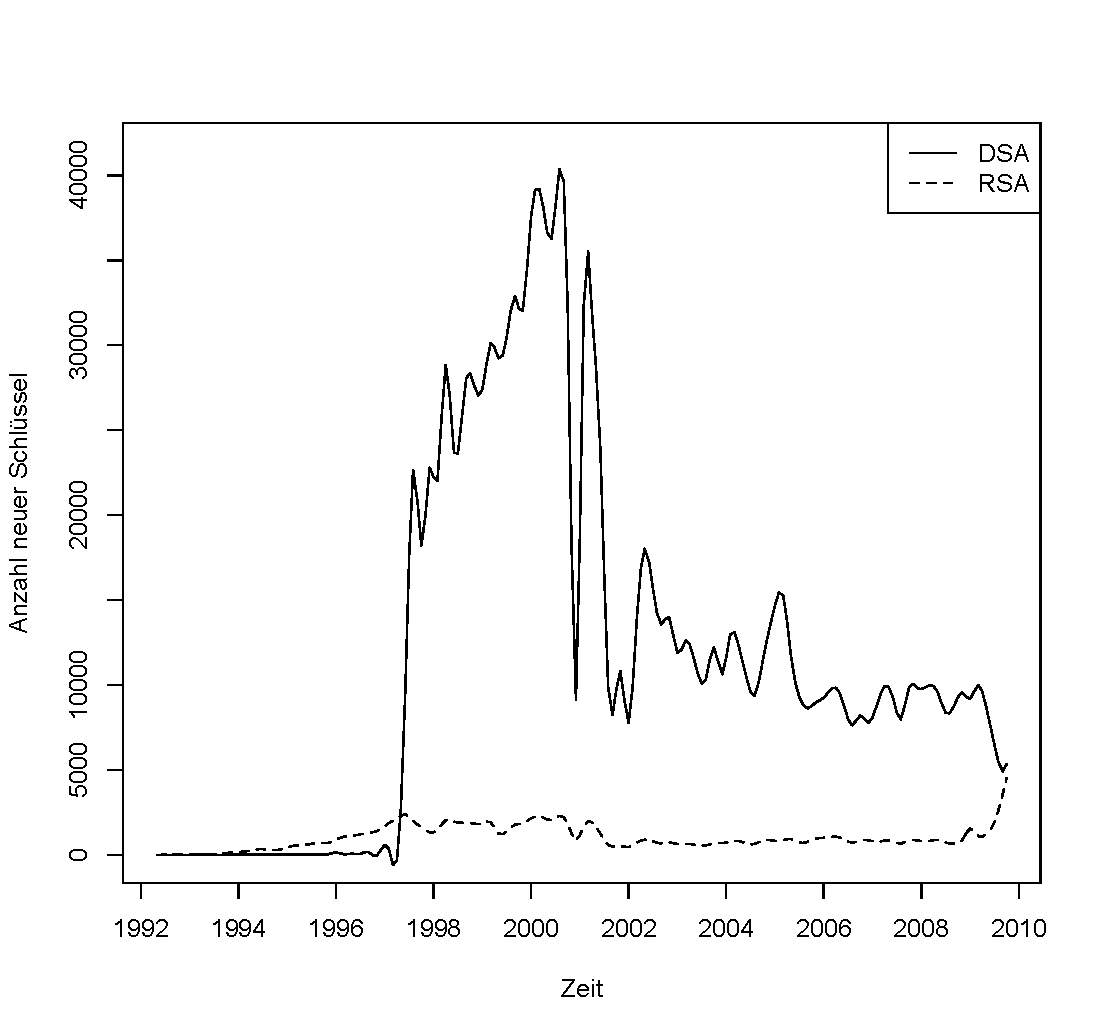
\includegraphics[scale=0.4]{images/whole-pkalg-use.pdf}}
  \subfloat[]{\label{fig:pkalg-mscc} 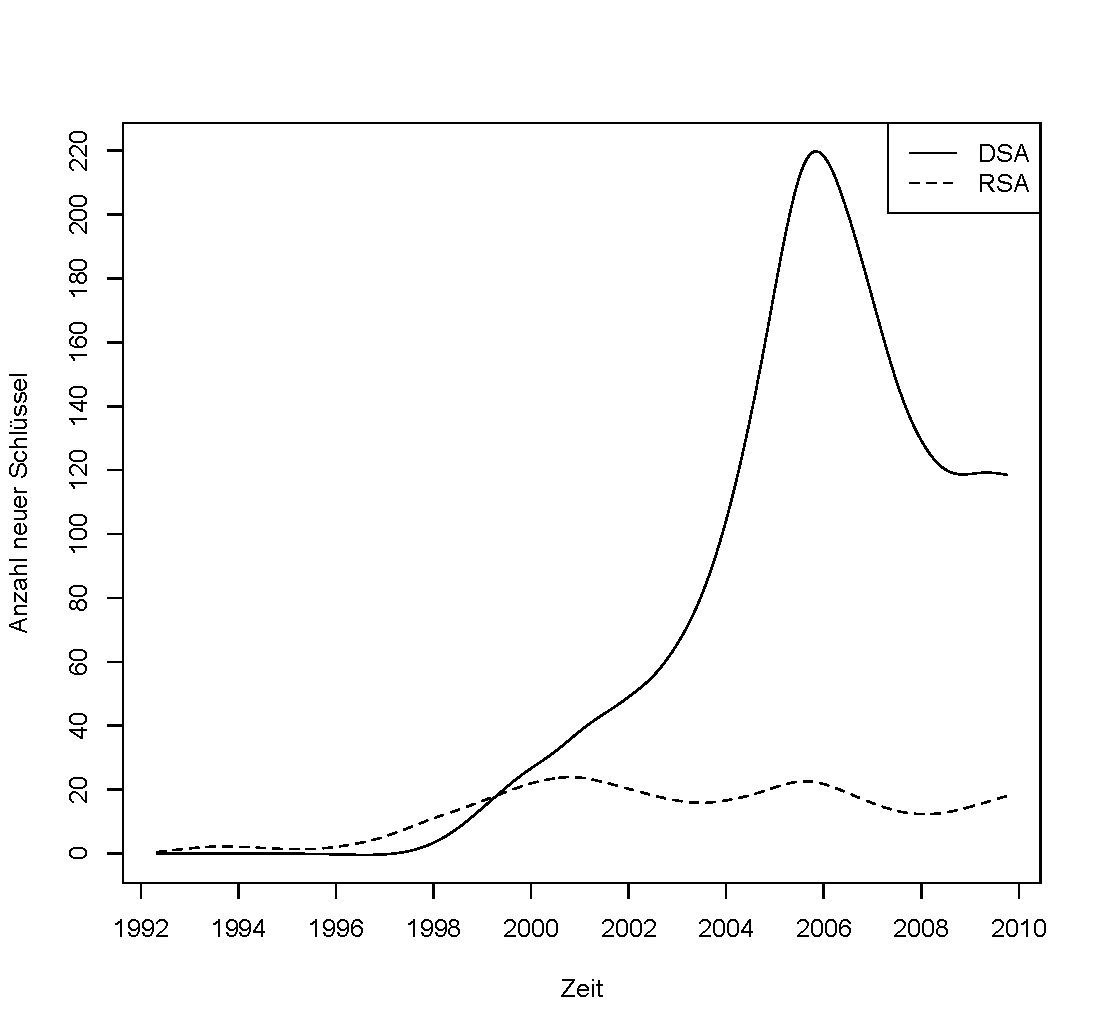
\includegraphics[scale=0.4]{images/mscc-pkalg-use.pdf}}
  \caption{Rate neuer PGP-Schl\"ussel, die RSA oder DSA benutzen,
    f\"ur den gesamten Schl\"usselbestand \subref{fig:pkalg-whole} und
    die gr\"osste starke Zusammenhangskomponente
    \subref{fig:pkalg-mscc} in monatlichen Abst\"anden}
  \label{fig:pkalg}
\end{figure}

Abbildung \ref{fig:size-dev} zeigt die Rate neuer Schl\"ussel,
abh\"angig von dem verwendeten Public-Key-Algorithmus. Die
DSA-Schl\"ussel machen zu jedem Zeitpunkt den gr\"ossten Anteil
aus. Ihre Entwicklung spiegelt im Wesentlichen die
Gr\"ossenentwicklung insgesamt aus Abbildung \ref{fig:size-dev}
wieder. Demgegen\"uber ist die Zuwachsrate von RSA-Schl\"usseln bis
zum Jahr 2008 konstant niedrig. Der Grund daf\"ur ist vermutlich, dass
die PGP-Implementierungen in diesem Zeitraum in der
Standardeinstellung DSA-Schl\"ussel erzeugten, was wiederum unter
anderem in dem bis ins Jahr 2000 bestehenden Patentschutz des
RSA-Algorithmus begr\"undet ist.  Die Rate neuer DSA-Schl\"ussel sinkt
ab dem Jahr 2009 deutlich ab, w\"ahrend die Rate neuer RSA-Schl\"ussel
gleichzeitig deutlich ansteigt. Vermutlich ist dies darauf
zur\"uckzuf\"uhren, dass seit dem Jahr 2009 neue Schl\"ussel, die mit
GnuPG erzeugt werden, in der Standardeinstellung RSA statt DSA
verwenden. Diese Umstellung wurde in der Entwicklerversion von GnuPG
am
17.05.2009\footnote{http://lists.gnupg.org/pipermail/gnupg-devel/2009-May/025079.html}
aufgrund von Berichten \"uber verbesserte Angriffe auf die
Hashfunktion SHA-1\cite{McDonald2009}, auf der DSA basiert,
vorgenommen. Warum diese Entwicklung nicht ebenfalls in der gr\"ossten
starken Zusammenhangskomponente sichtbar ist, ist nicht
klar. M\"oglicherweise liegt dies daran, dass f\"ur die Aufnahme in
diese Teilmenge nicht nur das Erzeugen eines Schl\"ussels, sondern
auch zus\"atzliche Aktitiv\"at in Form der Vernetzung mit anderen
Schl\"usseln notwendig ist. Neue Schl\"ussel werden also vermutlich im
Allgemeinen nicht sofort in die Zusammenhangskomponente aufgenommen,
sondern erst mit einiger Verz\"ogerung. Die Zusammenhangskomponente
d\"urfte also etwas ``tr\"ager'' auf Ver\"anderungen reagieren.

\subsection{Public-Key- und Hashalgorithmen}
\label{sec:public-key-und}

\begin{table}[ht!]
  \footnotesize
  \centering
  \subfloat{
    \label{tab:hash}
    \begin{tabular}[ht!]{l|c}
      Algorithmus & Anzahl \\
      \hline
      Signaturen gesamt & 446325 \\
      MD5 & 41700 \\
      SHA-1 & 398849 \\
      RIPE-MD/160 & 122 \\
      SHA256 & 5031 \\
      SHA512 & 2472 \\
      SHA224 & 532
    \end{tabular}
  }\quad
  \subfloat{
  \label{tab:algs}
    \begin{tabular}{l|c}
      Algorithmus & Anzahl \\
      \hline
      Schl\"ussel gesamt & 44952 \\
      RSA-512 & 203 \\
      RSA-768 & 257 \\
      RSA-1024 & 3903 \\
      RSA-2048 & 2408 \\
      RSA-3072 & 96 \\
      RSA-4096 & 1198 \\
      DSA & 36555
    \end{tabular}
  }\quad
  \subfloat{
    \label{tab:cert}
    \begin{tabular}{l|c}
      Cert Level & Anzahl \\
      \hline
      Generic & 299518 \\
      Persona & 904 \\
      Casual & 28718 \\
      Positive & 119575 
    \end{tabular}
  }
  \caption{Verwendung von Hashalgorithmen 
    \subref{tab:hash}, Public-Key-Algorithmen \subref{tab:algs} und
    Cert-Leveln \subref{tab:certs} in der gr\"ossten starken
    Zusammenhangskomponente}
\end{table}

In Tabelle \ref{tab:algs} sind schlussendlich noch einige Statistiken
\"uber Eigenschaften einzelner Schl\"ussel aufgef\"uhrt. 

Die einzelnen Cert level (siehe Abschnitt
\ref{ch:Grundlagen:sec:OpenPGP} werden durchaus verwendet (Tabelle
\ref{tab:certs}). Zwar ist
die Mehrheit der Signaturen mit dem Standardwert Generic versehen, der
keine weitere Aussage macht. Allerdings verf\"ugt \"uber 25\% der
Signaturen \"uber den h\"ochsten Wert Positive. Da die einzelnen Cert
level keine im Standard festgelegte klare Semantik haben, ist die
Aussagekraft dieser Werte nat\"urlich begrenzt. Sie k\"onnen aber
zumindest dahingehend interpretiert werden, dass \emph{mindestens} die
Personen, die von Generic abweichende Werte vergeben, den
Signaturprozess durchaus ernstnehmen.

Wie zu erwarten basiert die grosse Mehrheit der Signaturen in der
gr\"ossten starken Zusammenhangskomponente auf SHA1. Neben einzelnen
Signaturen mit Vertretern der SHA2-Familie findet sich aber auch noch
eine \"uberraschend hohe Anzahl von MD5-Signaturen: 41700 Signaturen,
d.h. 10\% basieren auf MD5. Die Sicherheit von MD5 muss inzwischen als
ernsthaft kompromittiert eingestuft werden. 2008 gelang es einer
Gruppe, durch eine Chosen-Prefix-Kollision ein von einer kommerziellen
CA signiertes ``b\"osartiges'' Certification-Authority-Zertifikat
f\"ur SSL zu erhalten \cite{Stevens2009}. GnuPG warnt zwar vor der
Verwendung von MD5-Signaturen, erlaubt ihre Verwendung aber noch. Die
Bedeutung der MD5-Signaturen f\"ur den Zusammenhalt der gr\"ossten
Komponente ist nicht unwesentlich: Werden diese Signaturen entfernt,
reduziert sich die Gr\"osse der Komponente auf 37599 Schl\"ussel,
d.h. es werden ca. 8000 Schl\"ussel abgetrennt. 

RSA-Schl\"ussel mit einer L\"ange von h\"ochstens 768 bit und weniger
m\"ussen ebenfalls als praktikabel brechbar betrachtet werden. Dies
wurde durch die Faktorisierung der Zahl RSA-768 demonstriert
\cite{Kleinjung2010}. Kleinjung et al. sch\"atzen den Zeitrahmen bis
zur Faktorisierung einer 1024-bit-Zahl innerhalb eines
\emph{akademischen Rahmens} auf 5 bis 10 Jahre. Die Menge der in der
gr\"ossten Komponente vorhandenen RSA-Schl\"ussel mit 512 bzw. 768 bit
ist mit insgesamt 450 Schl\"usseln gering. Ihre Entfernung trennt nur
etwa weitere 300 Knoten von der Komponente ab. Die Anzahl von
RSA-Schl\"usseln mit 1024 bit ist aber deutlich gr\"osser. Die
Entfernung aller ca. 4500 RSA-Schl\"ussel, deren L\"ange h\"ochstens
1024 bit betr\"agt, reduziert die Gr\"osse der Komponente um insgesamt
ca. 8500 Knoten, trennt also weitere 4000 Knoten vom Netz ab. Es ist
anzunehmen, dass sich die durchschnittlichen Distanzen ebenfalls
erh\"ohen. Da Standardorganisationen eine Abkehr von RSA-1024 ab dem
Jahr 2010
empfehlen\cite{NIST2007} und praktikable Angriffe wohl nur eine Frage
weniger Jahre sind, ist damit wie durch die MD5-Signaturen eine
erhebliche Beeintr\"achtigung der gr\"ossten Komponente absehbar.

Es ist zu erwarten, dass sich durch die Umstellung der
Standardeinstellung in GnuPG der Anteil von RSA-Schl\"usseln mit
einer L\"ange von mindestens 2048 bit in n\"achster Zeit deutlich
erh\"oht.

\section{Communities}
\label{sec:result-zusamm-und-comm}

Die Zerlegung des gerichteten Graphen mit dem Algorithmus von Rosval
et al. lieferte keine verwertbaren Ergebnisse. Zwar wurde eine
Zerlegung in 2869 Partitionen berechnet. Allerdings gilt f\"ur die
grosse Mehrzahl dieser Knotenmengen, dass der durch sie induzierte
Teilgraph \"uberhaupt keine Kanten hat. Nur f\"ur ca. 160 Partitionen
hat der jeweils induzierte Teilgraph Kanten, in allen F\"allen
allerdings sehr wenige (zwischen 1 und 104 f\"ur eine Partition der
Gr\"osse 682). Dass die Knoten einer Partition in allen F\"allen so
gut wie keine interne Vernetzung haben und damit der Definition von
Communities absolut nicht entsprechen, ist ein klarer Hinweis, dass
die berechnete Zerlegung die tats\"achliche modulare Struktur des
Graphen nicht sinnvoll wiedergibt. Dass der Graph in der Tat eine
ausgepr\"agte modulare Struktur hat, zeigen die anhand des
ungerichteten Graphen berechneten Zerlegungen, die auch unter
inhaltlichen Gesichtspunkten Sinn ergeben. Diese Struktur kann sich
auch nicht erst durch die Reduzierung des gerichteten auf einen
ungerichteten Graphen ergeben. Die berechnete Zerlegung mit etlichen
grossen Partitionen ohne interne Vernetzung ist in keinem Fall ein
sinnvolles Ergebnis eines Community-Algorithmus und spricht daher
f\"ur eine fehlerhafte Berechnung. Ob diese allerdings auf Fehler in
der verwendeten Implementierung der Autoren
\footnote{http://www.tp.umu.se/~rosvall/code.html} oder auf Fehler im
Algorithmus zur\"uckgeht, ist nicht bekannt.

F\"ur die restlichen Methoden wurde der Graph auf einen ungerichteten
Graphen reduziert. Dazu wurde jede einzelne gerichtete Kante in eine
ungerichte Kante umgewandelt. Aus dem gerichteten Graphen mit 446326
Kanten ergab sich so ein ungerichteter Graph mit 295425 Kanten.

F\"ur die COPRA-Berechnung wurden -- wie in \cite{Gregory2010}
vorgeschlagen -- Berechnungen mit unterschiedlichen Werten $v$
durchgef\"uhrt, um den ``besten'' Wert im Sinne der Modularity zu
ermitteln. Dabei ergaben sich mit steigender maximaler \"Uberlappung
$v$ nur bis $v\le 3$ steigende Modularity-Werte, dar\"uber hinaus
fielen sie kontinuierlich ab. Deshalb wurde die Berechnung mit $v=3$
verwendet. Die dort berechneten Modularity-Werte hatten eine geringe
Standardabweichung von 0,003. Dieses Ergebnis kommt unerwartet. In
\cite{Gregory2010} ergaben sich f\"ur ein PGP-Web-of-Trust-Netzwerk
mit 10680 Knoten bis zu $v=9$ ansteigende Modularity-Werte. Das
(lokale) Maximum bei geringem $v$ f\"ur das hier verwendete Netzwerk
k\"onnte darauf hinweisen, dass seine Community-Struktur keine
signifikante \"Uberlappung aufweist. Ein weiterer Hinweis darauf ist,
dass die Einf\"uhrung der \"Uberlappung mit $v=3$ gegen\"uber der
nicht \"uberlappenden Berechnung mit $v=1$ f\"ur die Modularity
(Tabelle \ref{tab:mod-result}) keinen signifikanten Anstieg
brachte. Auch die Zuordnung zu Gruppen bzw. Keysigning-Parties
(Tabelle \ref{tab:assign}) und die Verteilung der Gr\"osse der
Communities (Abbildungen \ref{fig:comsize-copra} und
\ref{fig:comsize-copra1}) \"ahneln sich weitgehend. Alternativ
k\"onnte dieses Ergebnis allerdings auch in einem nicht-optimalen
Verhalten des Algorithmus begr\"undet liegen.

\begin{figure}[th!]
  \centering
  \subfloat[]{\label{fig:comsize-copra1} 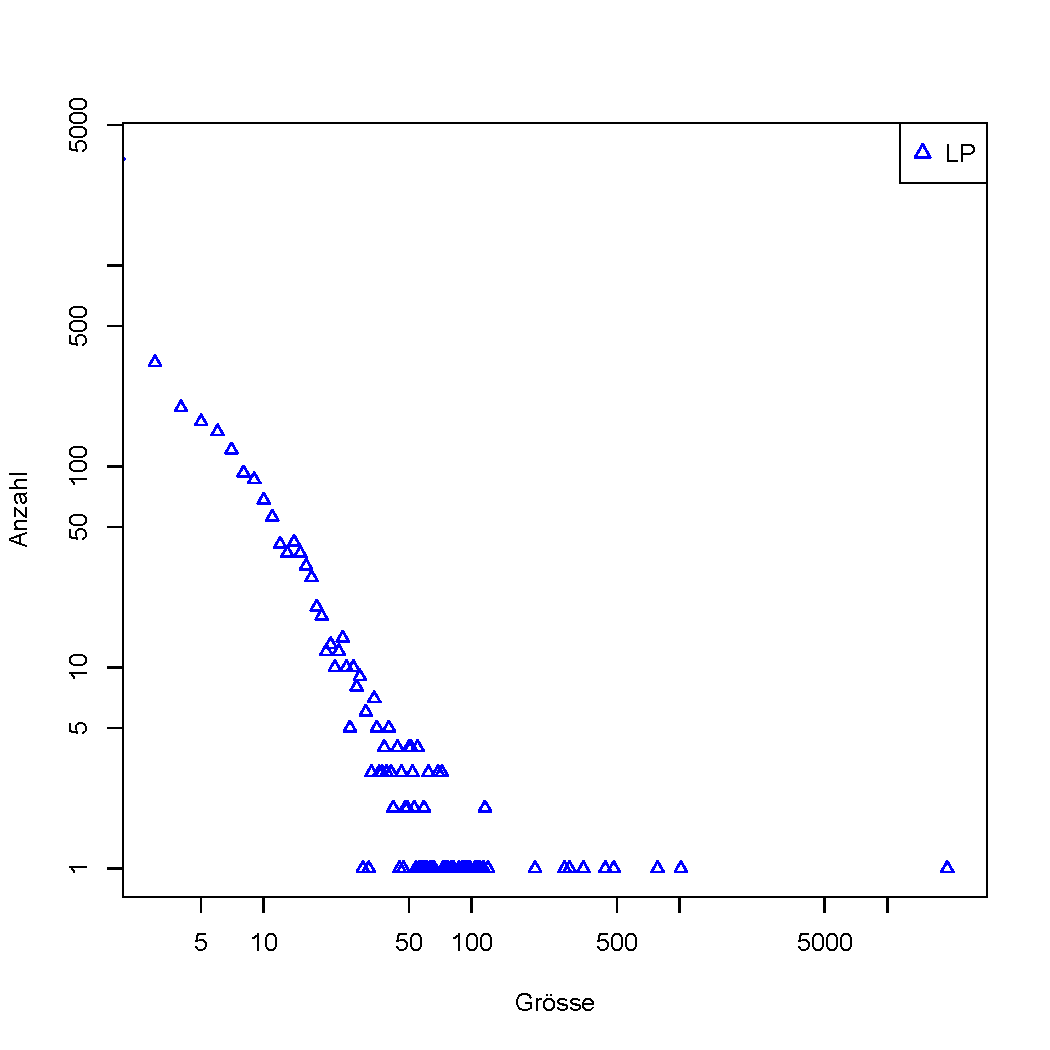
\includegraphics[scale=0.45]{images/community-size-dist_copra1.pdf}}
  \subfloat[]{\label{fig:comsize-copra} 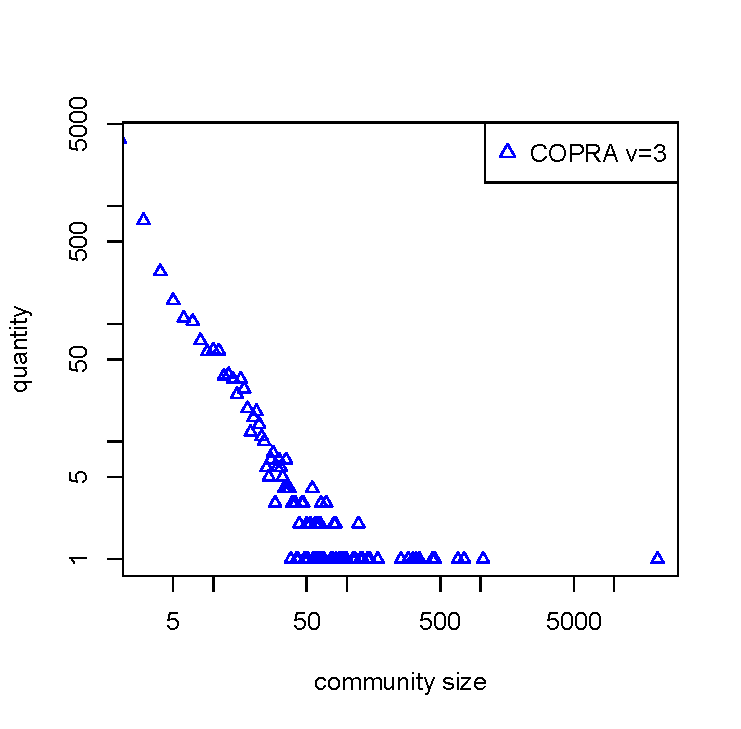
\includegraphics[scale=0.45]{images/community-size-dist_copra.pdf}} \\
  \subfloat[]{\label{fig:comsize-bl2} 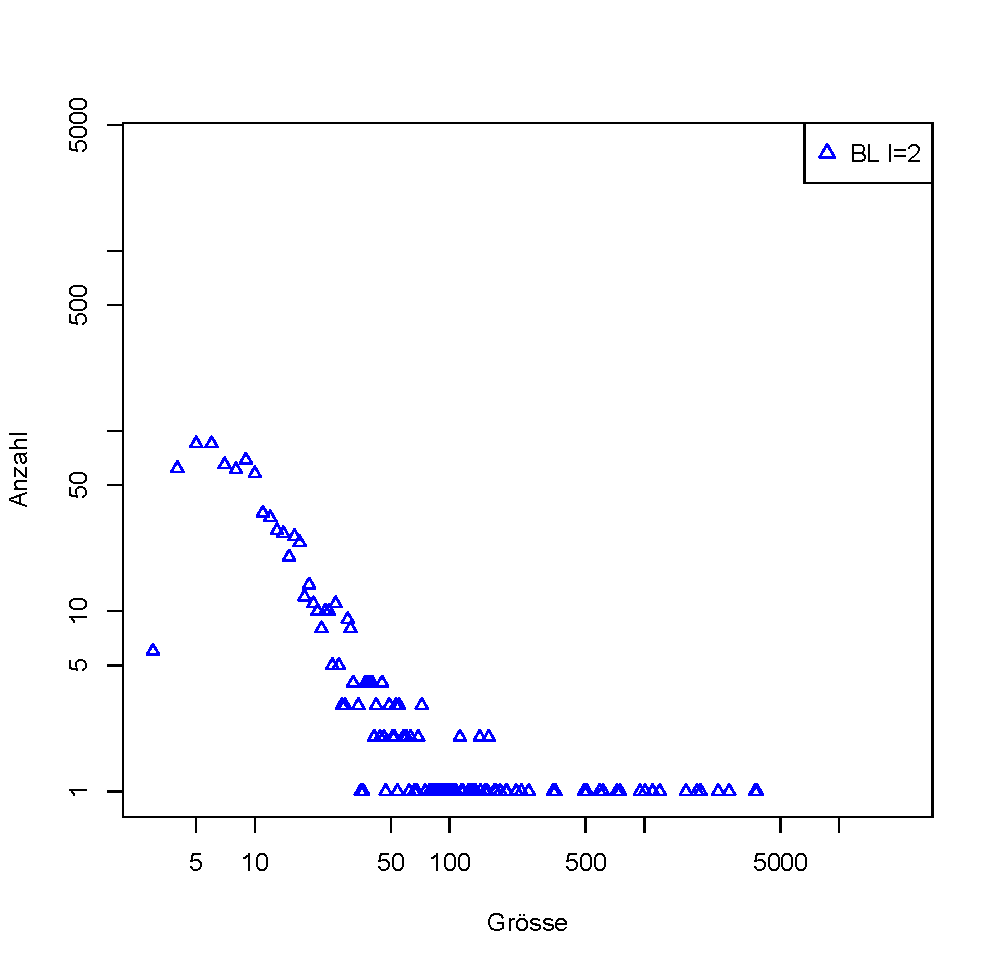
\includegraphics[scale=0.45]{images/community-size-dist_bl2.pdf}} 
  \subfloat[]{\label{fig:comsize-bl5} 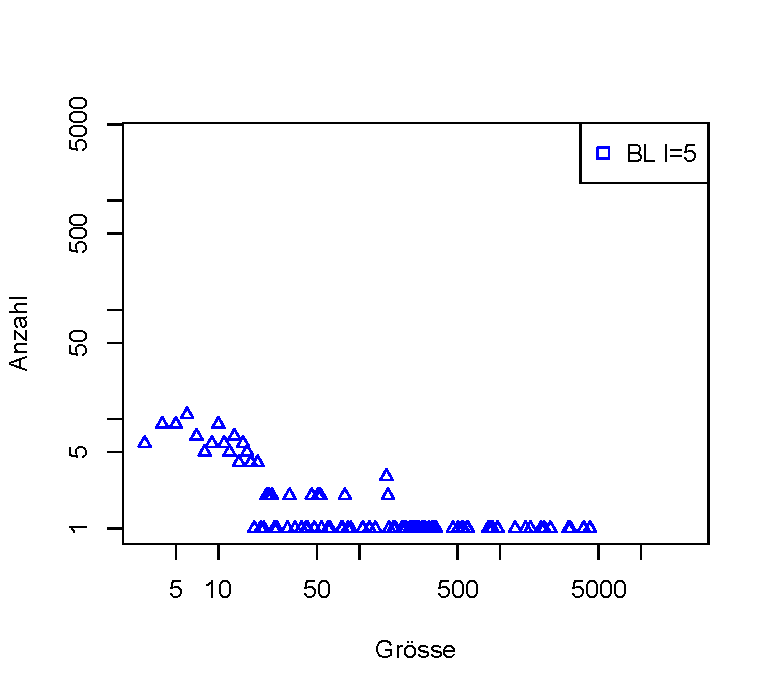
\includegraphics[scale=0.45]{images/community-size-dist_bl5.pdf}} 
  \caption{Gr\"ossenverteilung der Communities}
  \label{fig:comsizedist}
\end{figure}

F\"ur den Algorithmus von Blondel et al. zeigt sich zun\"achst ein
deutlich h\"oherer Modularity-Wert als f\"ur Fastmod. Dieses Ergebnis
gibt also die reine Struktur des Graphen deutlich besser wieder.  Wie
in Abschnitt
\ref{ch:Grundlagen:sec:Netzwerkanalyse:subsec:Communities}
beschrieben, verl\"auft der Algorithmus von Blondel et al. iterativ in
Phasen, in denen jeweils zuerst Knoten einer benachbarten Community
zugeordnet werden, wenn sich dadurch ein Modularity-Gewinn erzielen
l\"asst, und dann die Knoten dieser so entstandenen Communities zu
Knoten in einem neuen Netzwerk verschmolzen werden. Hier werden die
Ergebnisse der Phasen $l=2$ und der letzten Phase $l=5$
betrachtet. F\"ur $l=5$ ergab sich die h\"ochste
Modularity. Allerdings sticht hier die sehr kleine Anzahl von
Communities heraus, die wiederum vergleichsweise gross sein
m\"ussen. Gegen\"uber dem Ergebnis der Phase 2 ergibt sich eine
relativ kleine Steigerung der Modularity, die mit einem erheblichen
Verlust an \emph{Aufl\"osung} erkauft wird\footnote{Die Zerlegungen
  der Phasen 3 und 4 unterschieden sich nur geringf\"ugig von der
  Zerlegung der Phase 5}. Aus Abbildung \ref{fig:comsize-bl2} und
\ref{fig:comsize-bl5} geht hervor, dass diese Reduktion der Anzahl im
Wesentlichen auf das Reduzieren sehr kleiner Communities
zur\"uckgeht. Da der Algorithmus von Blondel et al. genauso wie
Fastmod mittels einer (lokalen) Optimierung der Modularity arbeitet,
k\"onnte dieses Ph\"anomen auf das in der Literatur beschriebene
Aufl\"osungslimit der Modularity-Funktion (bspw. \cite{Fortunato2007}
\cite{Good2009}) zur\"uckzuf\"uhren sein. Es scheint fraglich, ob die
in Relation zur Gr\"osse des Graphen sehr geringe Zahl von 186
Communities die Struktur des Graphen (in Bezug auf die inhaltliche
Analyse) ad\"aquat wiedergibt.

\begin{figure}[ht!]
  \centering
  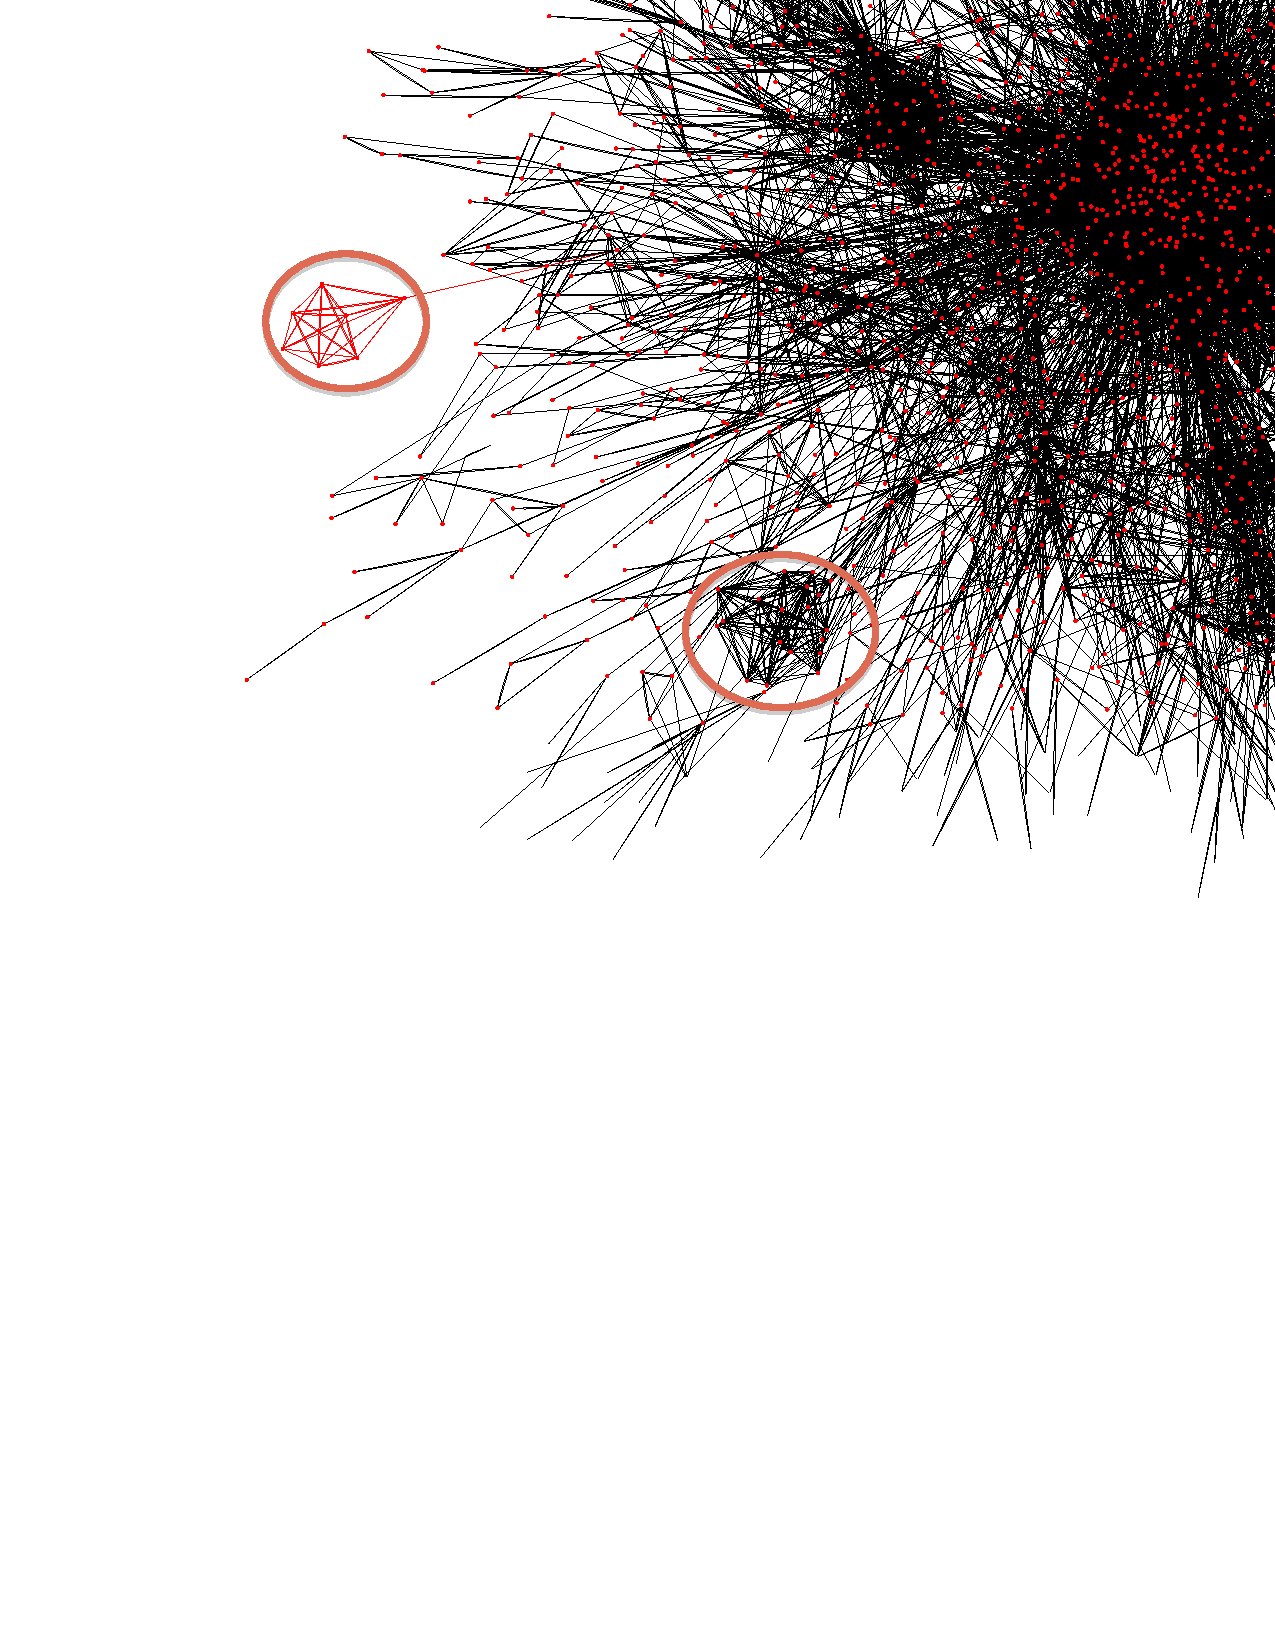
\includegraphics[scale=0.7]{images/blondel-l5-com-c3a5eaab680984b123037897b0be74bf-edit.pdf}
  \caption{Community mit modularen Untereinheiten (Gr\"osse 2271,
    Blondel ($l=5$), Force-directed Layout)}
  \label{fig:large-modular}
\end{figure}

Abbildung \ref{fig:large-modular} illustriert dies anhand einer
Community aus der Zerlegung des Algorithmus von Blondel et al. mit
$l=5$, die klar abgegrenzte Untereinheiten enth\"alt, die intuitiv
wieder eigenst\"andige Communities darstellen.

\begin{figure}[th!]
  \centering
  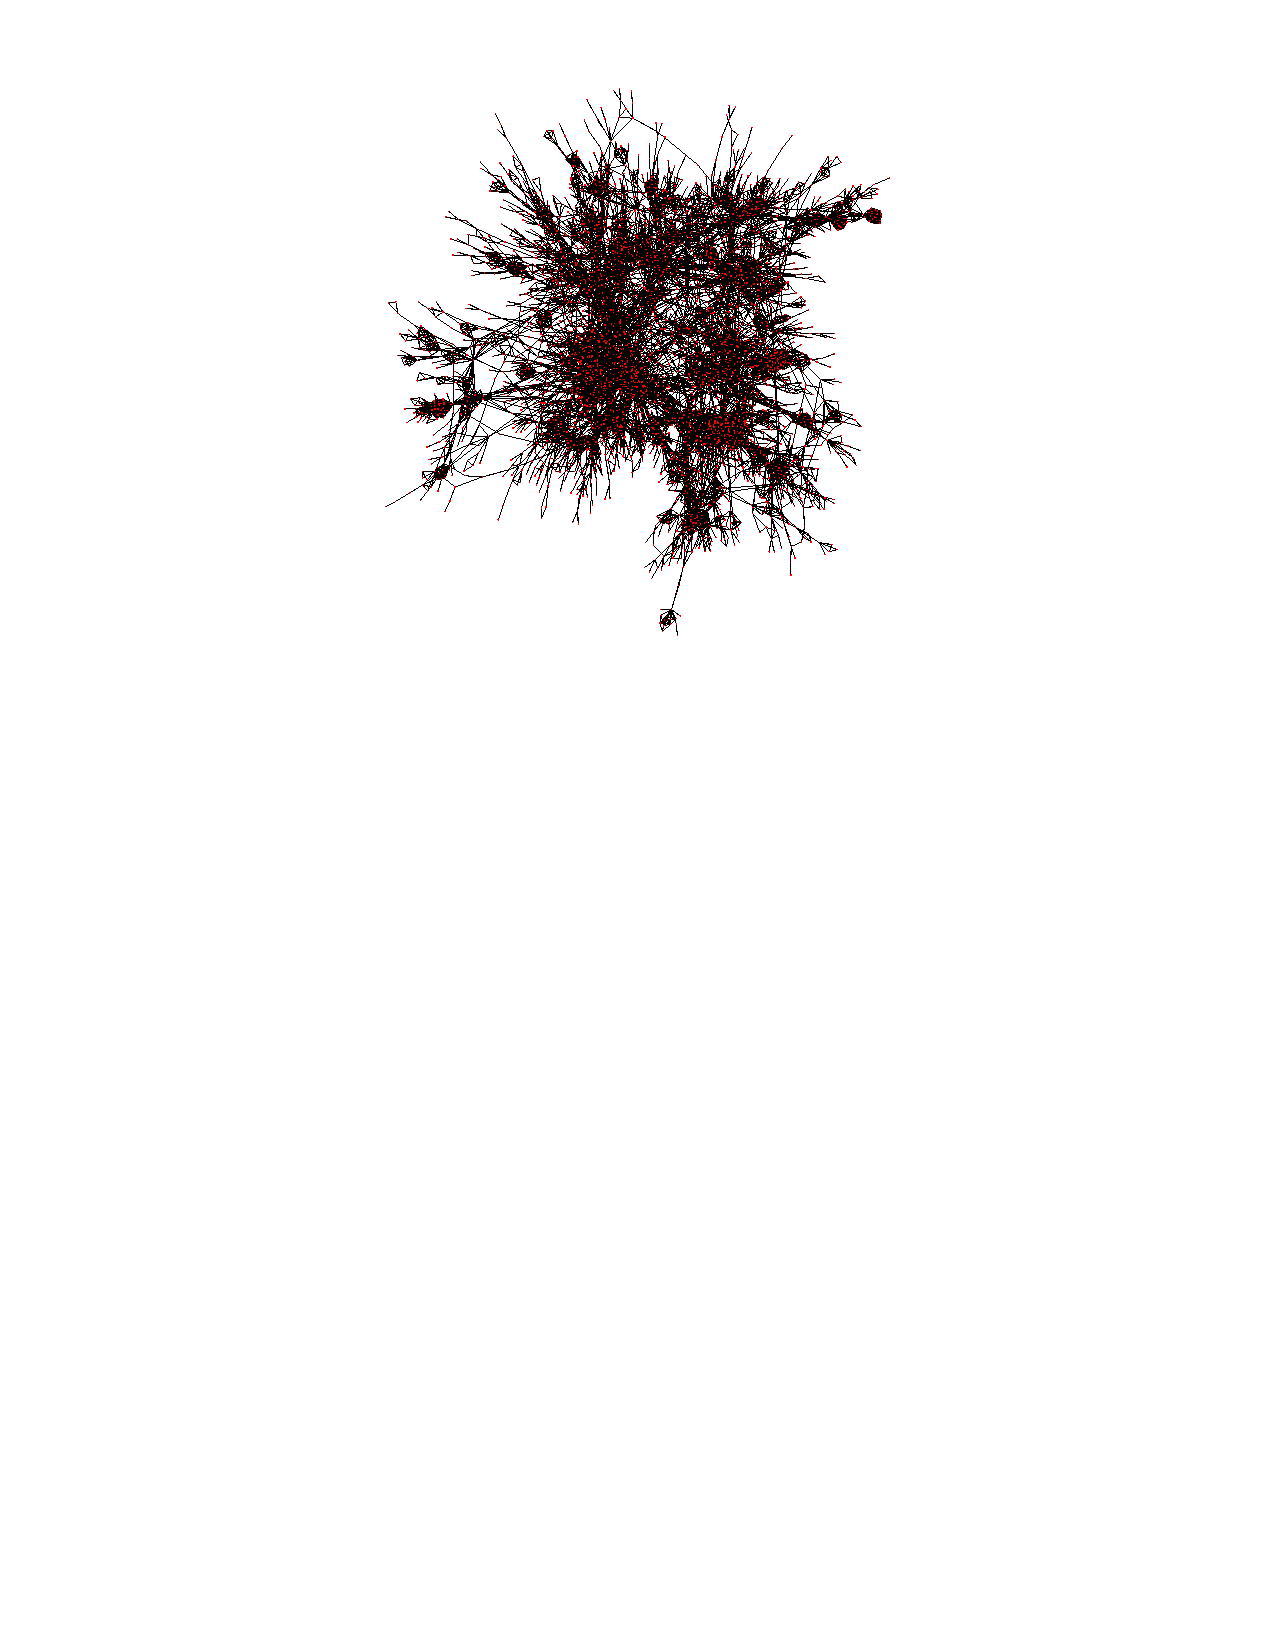
\includegraphics[scale=1.5]{images/fastmod-subgraph-large-modular-6525064ccab580a0b304a3620b197d7a.pdf}
  \caption{Grosse Community mit modularer Struktur (Berechnet mit
    Fast-Modularity, Force-directed layout)}
  \label{fig:large-community-modular}
\end{figure}

Abbildung \ref{fig:large-community-modular} illustriert die begrenzte
Qualit\"at der Fast-Modularity-Zerlegung, die sich im vergleichweise
niedrigen Modularity-Wert niederschl\"agt. In der Zeichnung des
induzierten Teilgraphen einer grossen Community sind etliche dicht
gezeichnete Zusammenballungen von Knoten zu sehen, die nur wenige
Kanten nach aussen haben. Diese k\"onnen als Community-artige
Strukturen interpretiert werden. Zwar kann argumentiert werden, dass
die Zeichnung die Struktur des Teilgraphen nicht notwendigerweise
sinnvoll wiedergibt, dass also die dichten Teilbereiche in der
Zeichnung nur Artefakte der Zeichenmethode darstellen. Allerdings
zeigt Noack, dass starke \"Ubereinstimmungen zwischen einer
energieoptimalen Einbettung eines Graphen in die Ebene nach der
Force-directed-Methode und einer Partitionierung eines Graphen mit
optimaler Modularity bestehen \cite{Noack2009}. Es scheint daher
gerechtfertigt, eine Zeichnung eines Graphen (Force-directed) mit
markanten dichten Bereichen als Indiz f\"ur eine modulare Struktur
dieses Graphen zu betrachten.

Die Verteilungen der Community-Gr\"ossen aus allen Berechnungen sind
in einer Hinsicht konsistent: Neben einer grossen Zahl von kleinen
Communities gibt es eine signifikante Anzahl von gr\"osseren bis sehr
grossen Communities. Es scheint also keine charakteristische Gr\"osse
der Communities zu geben.

\begin{table}[t]
  \centering
  \footnotesize
  \begin{tabular}{l|c|c|c}
    Algorithmus & Modularity & Communities &
    Enthaltene Knoten \\
    \hline
    FM & 0,596 & 552 & 44611 \\
    \hline
    BL ($l=2$)& 0,701 & 936 & 44934 \\
    BL ($l=5$)& 0,710 & 186 & 44934 \\
    \hline
    COPRA ($v=1$) & (0,780) & 1421 & 42205 \\
    COPRA ($v=3$) & (0,786) & 1354 & --- \\

  \end{tabular}
  \caption{Modularity-Werte, Anzahl der Communities mit mehr als 3
    Knoten sowie die Anzahl der insgesamt in diesen Communities (>3) enthaltenen
    Knoten 
    f\"ur die Algorithmen Fast-Modularity (FM), Label-Propagation
    (LP), Blondel et al. (BL) auf Level 2 und 5 sowie COPRA. Die
    Modularity-Werte f\"ur COPRA entsprechen der Modularity-Definition
    f\"ur \"uberlappende Zerlegungen nach \cite{Nicosia2009} und k\"onnen mit den anderen
    Werten nicht verglichen werden.}
  \label{tab:mod-result}
\end{table}

Aus Tabelle \ref{tab:mod-result} geht hervor, dass sich -- zumindest
im Fall von Fastmod und Blondel et al. -- fast alle Knoten des Graphen
in einer Community wiederfinden, die mindestens die Gr\"osse 4 hat. In
Abschnitt \ref{sec:result-allg-merkm-des} wurde gezeigt, dass ein
erheblicher Anteil der Knoten einen sehr geringen Grad von 1 oder 2
hat. Da solche Knoten mangels Kanten nicht selbst eine dichte
Vernetzung herstellen k\"onnen, m\"ussen sie Mitglied in Communities
sein, in denen Knoten mit h\"oherem Grad sowohl die interne Vernetzung
der Community als auch die Vernetzung der Community mit anderen
erzeugen. COPRA scheint hingegen dazu tendieren, deutlich mehr Knoten
in Communities sehr kleiner Gr\"osse mit 3 oder weniger
unterzubringen. Dieses Verhalten k\"onnte dazu f\"uhren, dass die
Aussagekraft der Zerlegung in Bezug auf die realen Communities
geschw\"acht wird, wenn viele Knoten auf diese Art abgespalten werden.

Gegen\"uber der COPRA-Zerlegung mit $v=1$ zeigt die Zerlegung mit
$v=3$ eine deutlich gr\"ossere Anzahl von Communities der Gr\"osse 3
und 4. Abgesehen davon \"ahneln sich die Gr\"ossenverteilungen aber
weitgehend. Beide enthalten eine charakteristische sehr grosse
Community mit ca. 19000 bzw. ca. 21000 Mitgliedern. Demgegen\"uber
bietet die Blondel-Zerlegung mit $l=2$ eine deutlich geringere Anzahl
solcher sehr kleiner Communities, daf\"ur aber eine h\"ohrere Zahl
mittlerer (mehr als 100 Mitglieder) und insbesondere eine h\"ohere
Zahl sehr grosser (zwischen 500 und 5000 Mitglieder) Communities.  Die
beiden Algorithmen konvergieren nicht gegen ein gemeinsames Optimum,
sondern liefern Ergebnisse, die sich qualitativ stark unterscheiden.

Der insgesamt recht hohe Modularity-Wert weist darauf hin, dass der
Graph in der Tat eine ausgepr\"agte modulare Struktur hat, wie dies
von einem sozialen Netzwerk erwartet wird. Newman et al. geben an,
dass ein Modularity-Wert $C \ge 0.3$ in der Praxis auf eine
signifikante Community-Struktur schliessen l\"asst\cite{Clauset2004}.

Die Abbildungen \ref{fig:metagraph-com-copra} und
\ref{fig:metagraph-com-blondel2} zeigen die Struktur der Communities
f\"ur die Zerlegungen COPRA ($v=1$) und Blondel ($l=2$). Auff\"allig
ist hier insbesondere die teilweise sternf\"ormige Struktur der
COPRA-Zerlegung. Ein signifikanter Anteil der kleineren Communities
ist rund um die zentrale Community der Gr\"osse ca. 19000 angeordnet
und im wesentlichen nur mit dieser vernetzt. Diese Struktur weist
gewisse \"Ahnlichkeiten zur Struktur der starken
Zusammenhangskomponenten auf (siehe Abschnitt
\ref{sec:result-komponentenstruktur}). Diese sind ebenfalls sternf\"ormig um
eine zentrale Komponente angeordnet, die die Gr\"osse der anderen um
mehrere Gr\"ossenordnungen \"ubertrifft. Allerdings sind im Fall der
Community-Struktur noch eine Reihe mittelgrosser Communities
vertreten, die dieses Muster etwas st\"oren. Das sternf\"ormige Muster
der Zusammenhangskomponenten wiederholt sich also in etwa innerhalb
der gr\"ossten Zusammenhangskomponente auf einem anderen Level. Es
k\"onnte daher spekuliert werden, ob das Netzwerk eine
\emph{Selbst\"ahnlichkeit} aufweist, wie sie f\"ur eine Reihe von
komplexen Netzwerken gezeigt wurde\cite{Song2005}. Dieser Frage wurde
allerdings im Rahmen dieser Arbeit nicht weiter nachgegangen. Im
Vergleich dazu zeigt sich in der Struktur der Blondel-Communities die
etwas ausgewogenere Gr\"ossenverteilung. Zwar sind auch hier viele
kleine Communities sternf\"ormig um die zentralen Communities
angeordnet, verteilen sich hier aber auf mehrere solcher grossen
zentralen Communities.

\begin{figure}[h!]
  \centering
  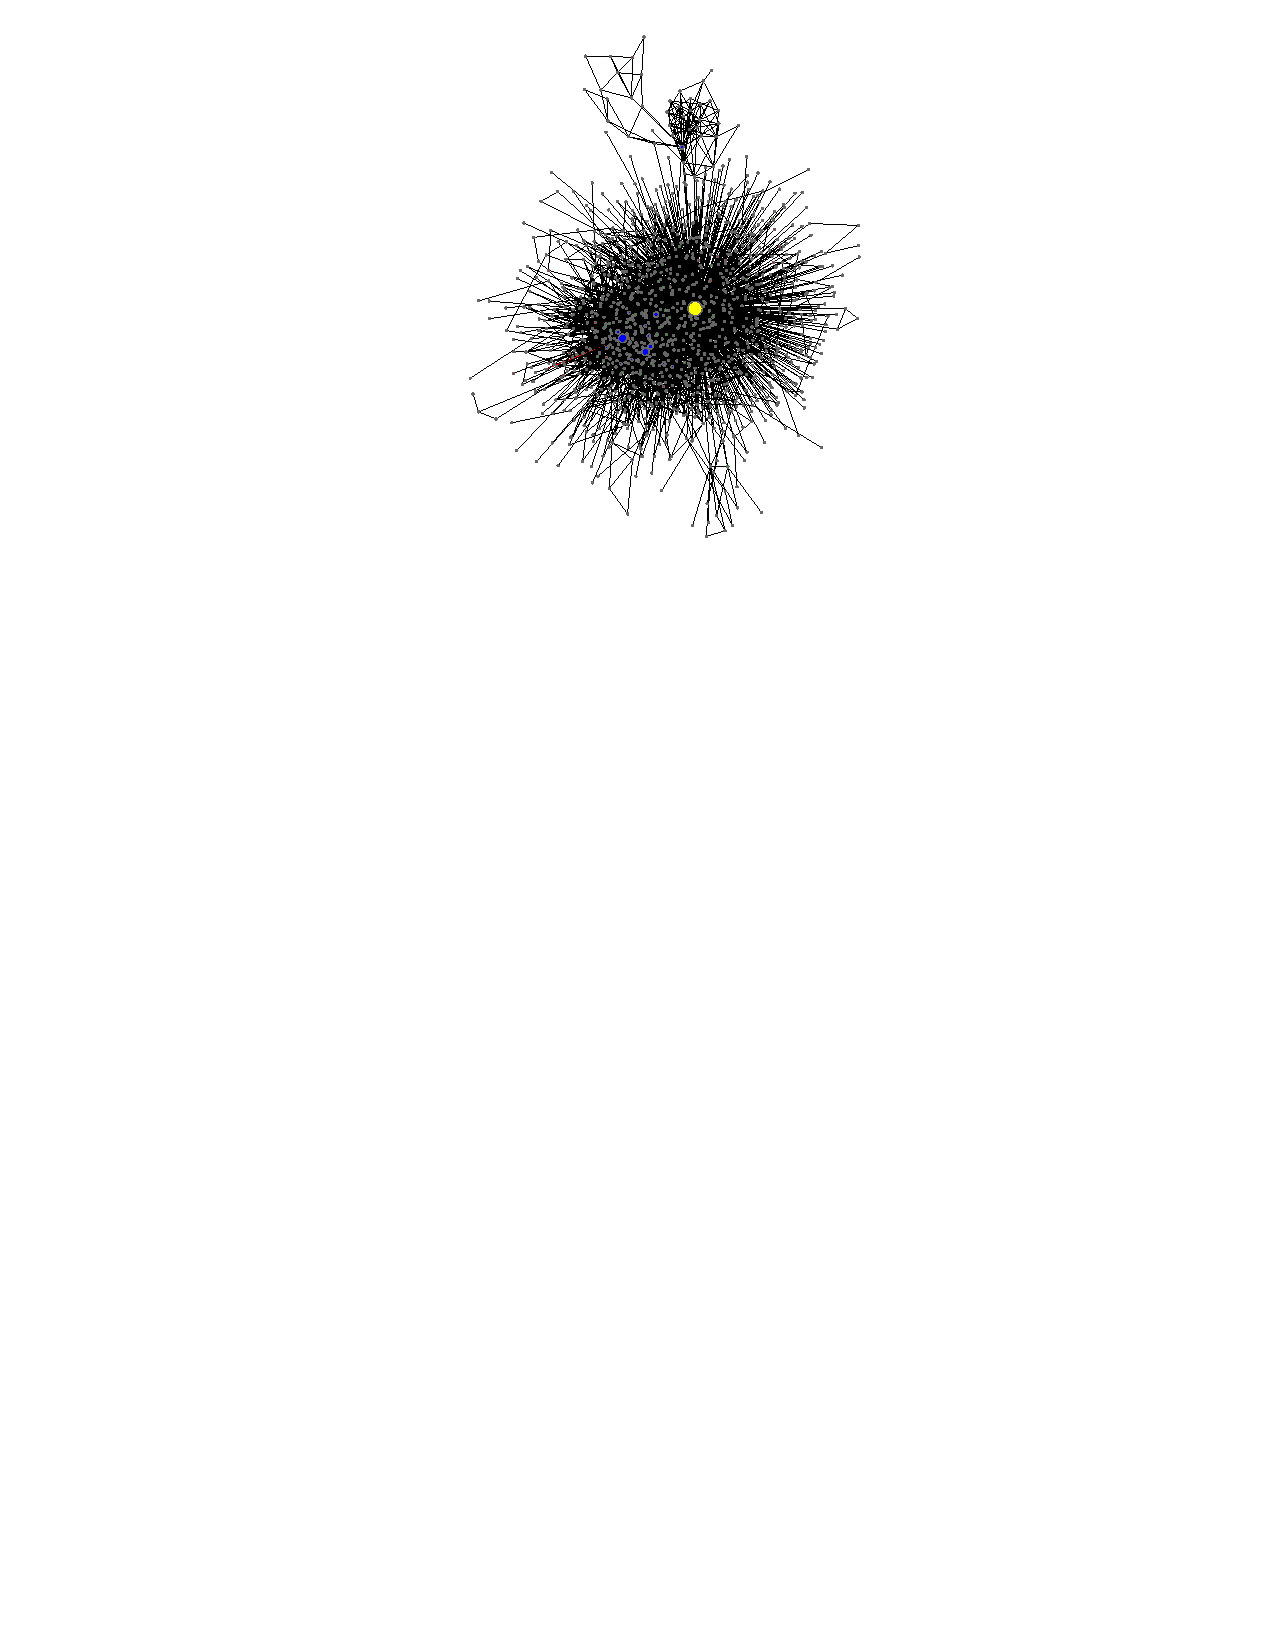
\includegraphics[scale=2]{images/metagraph-copra1-minsize5.pdf}
  \caption{Struktur der Communities (COPRA ($v=1$) (rot: Gr\"osse
    $<10$, gr\"un: Gr\"osse $<100$, blau: Gr\"osse < 1000, gelb:
    Gr\"osse > 1000).}
  \label{fig:metagraph-com-copra}
\end{figure}

\begin{figure}[h!]
  \centering
  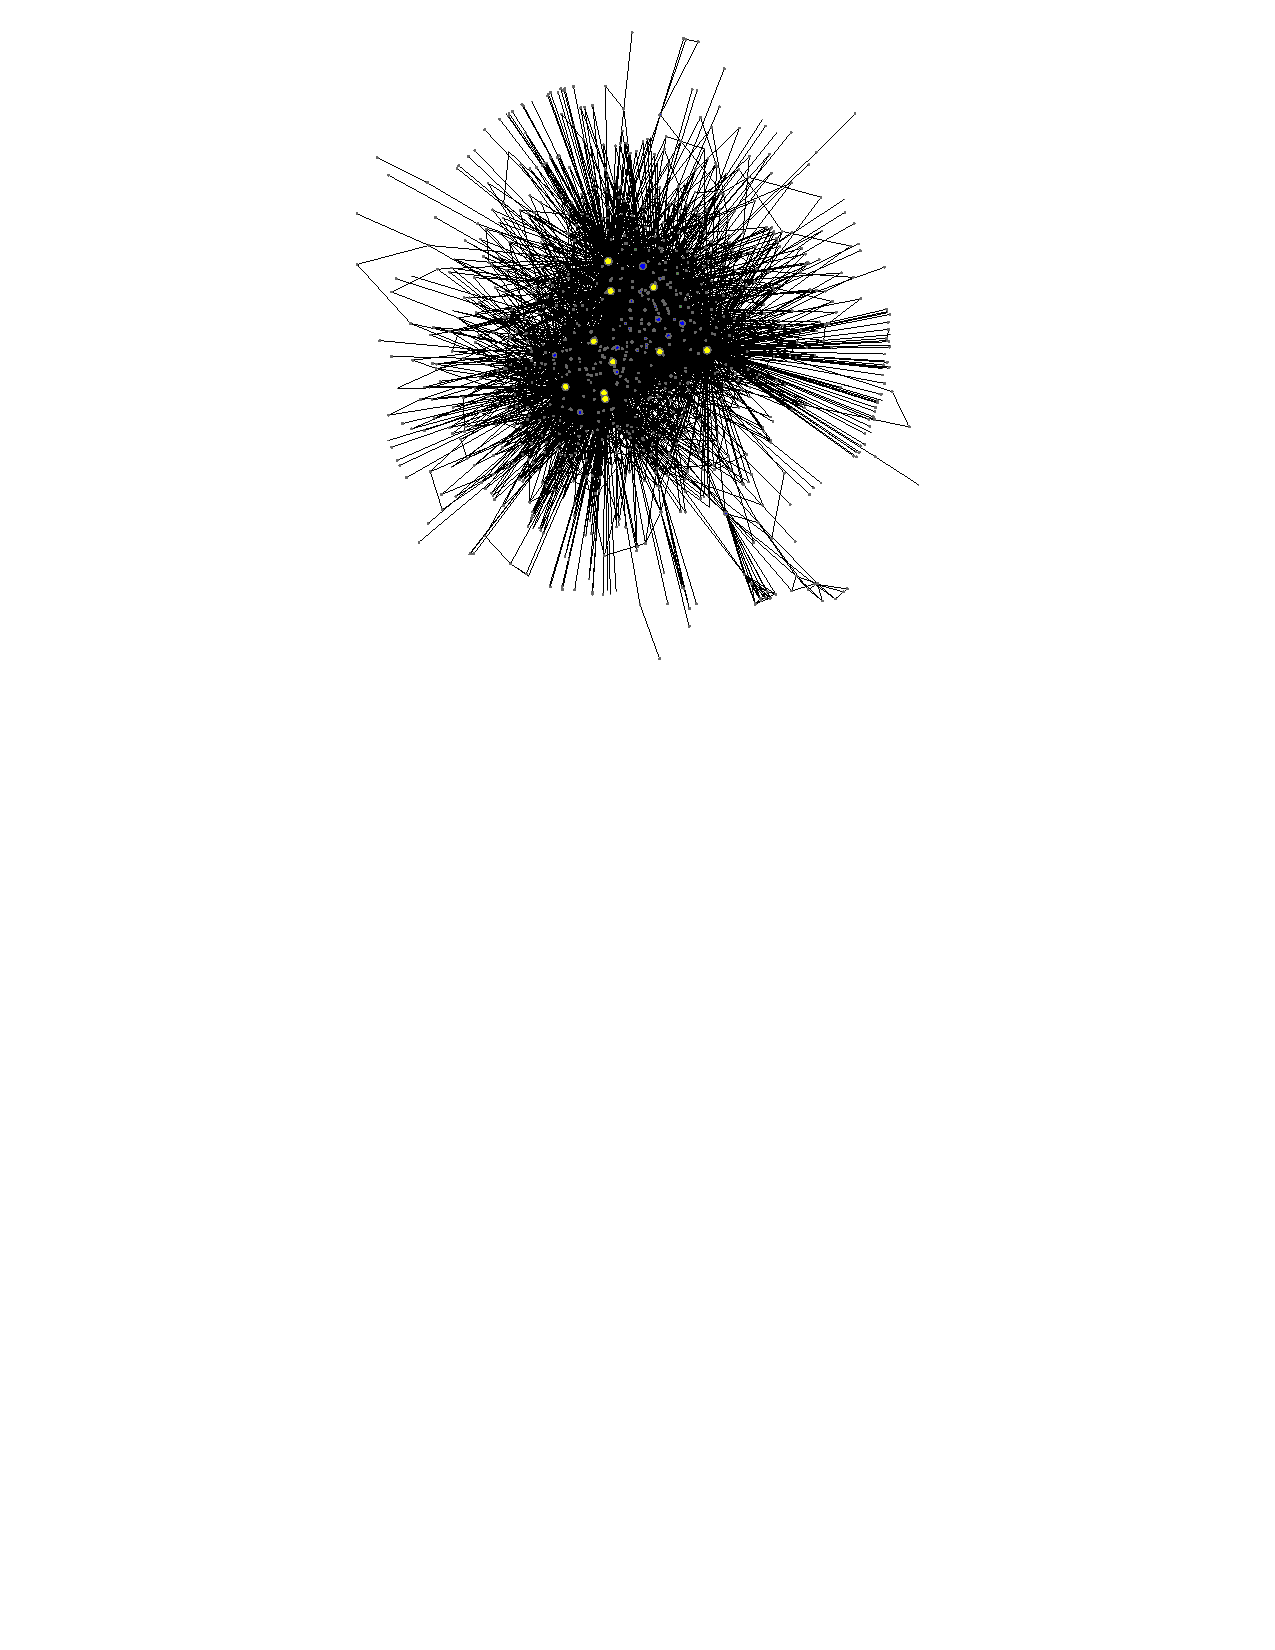
\includegraphics[scale=1.6]{images/metagraph-blondel2-minsize4.pdf}
  \caption{Struktur der Communities (Blondel ($l=5$) (Knotenf\"arbung
    wie in Abb.\ref{fig:metagraph-com-copra})}
  \label{fig:metagraph-com-blondel2}
\end{figure}

\begin{table}[t]
  \centering
  \footnotesize
  \begin{tabular}{l|c|c|c|c|c}
    Algorithmus & TLD-S & TLD-M & SLD-S & SLD-M & SIG \\
    \hline
    FM & 293 (53\%) & 247 (44\%) & 56 (10\%) & 154 (27\%) & 128
    (23\%) \\
    \hline
    BL ($l=2$) & 499 (53\%) & 417 (45\%) & 41 (4\%) & 254 (27\%) & 115 (12\%) \\
    BL ($l=5$) & 85 (47\%) & 85 (47\%) & 15 (8\%) & 38 (21\%) & 26 (14\%) \\
    \hline
    COPRA ($v=1$) & 824 (58\%) & 564 (40\%) & 178 (13\%) & 429 (30\%)
    & 572 (40\%) \\
    COPRA ($v=3$) & 792 (58\%) & 525 (38\%) & 187 (14\%) & 425 (31\%) & 555
    (41\%)
  \end{tabular}
  \caption{SLD-TLD-Zuweisung, TIME-CORR}
  \label{tab:assign}
\end{table}

Aus Tabelle \ref{tab:assign} geht hervor, dass f\"ur alle Zerlegungen
fast alle Communities einer Top-Level-Domain zuordnenbar sind oder von
einer TLD dominiert werden. Werden die generischen Top-Level-Domains
(gTLD: com, org, net, info, ...) abgezogen, verbleiben im Fall von COPRA
noch 519 (38\%) Communities, die einer TLD (und damit einer
\emph{Country-Coded TLD (ccTLD)}) zugeordnet werden k\"onnen und 315
(23\%), die von einer ccTLD dominiert werden. F\"ur die anderen
Zerlegungen ergeben sich \"ahnliche Werte. Damit ist immerhin etwa die
H\"alfte der Communities einem Land zuordnenbar. F\"ur die von einer
gTLD dominierten Communities ergeben Stichproben, dass sich die
Teilnehmer der meisten dieser Communities anhand der Namen zumindest
einem Sprachraum zuweisen lassen.

Dieses Ergebnis ist naheliegend. Wie in Abschnitt
\ref{sec:community-analyse} dargelegt, wird davon ausgegangen, dass
ein wesentlicher Faktor, der das Zustandekommen von Signaturen
beeinflusst, die sozialen Kontakte einer Person sind. Es ist weiterhin
naheliegend, dass sich diese sozialen Kontakte unter anderem aufgrund
von Sprachbarrieren und der r\"aumlichen N\"ahe haupts\"achlich im
Rahmen eines Landes ergeben. Beispielsweise ist f\"ur eine aus
Finnland stammende Person anzunehmen, dass die Mehrzahl ihrer Freunde,
Bekannten, Gesch\"aftspartner und sonstigen Kontakte wieder Finnen
sind.

Zwar k\"onnte argumentiert werden, dass das Internet die geographische
bzw. nationale Beschr\"ankung sozialer Kontakte aufhebt. Allerdings
spielt die geographische N\"ahe eine wichtige Rolle im
Signaturprozess. Die verbreitete Prozedur f\"ur das Signieren eines
Schl\"ussels setzt ein direktes pers\"onliches Treffen der
Signierenden voraus (siehe Abschnitt \ref{sec:sozi-komp-des}). Es ist
anzunehmen, dass die \"uberwiegende Mehrheit der PGP-Benutzer die
meiste Zeit in einem Land und damit in einem geographisch
eingegrenzten Bereich verbleibt. Damit kommen f\"ur diese Mehrheit
\"uberwiegend nur Bewohner des gleichen Landes als Signaturpartner in
Frage. Als Mechanismen f\"ur die internationale Vernetzung kommen dann
etwa internationale Konferenzen in Frage. Nur ein sehr kleiner Teil
der PGP-Benutzer d\"urfte die notwendige internationale Mobilit\"at
aufweisen, so dass sich seine Signaturen nicht \"uberwiegend einem
geographischen Bereich bzw. einem Land zuweisen lassen.

Interessanter f\"ur die Fragestellung ist aber die Erkennung von
Keysigning-Parties und die Zuordnung zu Second-Level-Domains. Im
Vergleich der Algorithmen (Tabelle \ref{tab:assign}) zeigt sich
zun\"achst, dass die COPRA-Zerlegungen bessere Resultate liefern als
die Blondel-Zerlegungen, da hier mehr Communities zugeordnet werden
k\"onnen. Zwar entf\"allt bei COPRA ein grosser Anteil dieser
Zuordnungen auf sehr kleine Communities der Gr\"osse 3 und 4. Die
Aussagekraft solcher kleiner Zuordnungen ist selbstverst\"andlich sehr
begrenzt. Werden diese abgezogen, verbleibt aber immer noch eine
gr\"ossere Zahl zuordnenbarer Communities nichttrivialer Gr\"osse. Aus
den absoluten Zahlen in Tabelle \ref{tab:assign} und den
Gr\"ossenverteilungen in Abbildungen \ref{fig:sld-suredist},
\ref{fig:sld-maybedist} und \ref{fig:time-corrdist} geht hervor, dass
die \"Uberlappung keine wesentlichen Vorteile bringt. Im Vergleich der
Blondel-Zerlegungen zeigt sich, dass das Zusammenpacken von
Communities von Phase $l=2$ zu Phase $l=5$ und der damit verbundene
Aufl\"osungsverlust es erheblich erschwert, die Communities inhaltlich
zuzuordnen. Eine Zerlegung mit h\"oherer Modularity entspricht also im
Allgemeinen nicht einer Zerlegung, die die Struktur realer Communities
besser wiedergibt. Die Zerlegungen des Algorithmus von BLondel et
al. scheinen insgesamt vom Aufl\"osungslimit der
Modularity-Maximierung betroffen zu sein und bieten daher nicht die
notwendige Aufl\"osung, um die Communities besser inhaltlich
analysieren zu k\"nnen.

Insgesamt ist eine tats\"achliche Zuordnung anhand des
80\%-Schwellwerts nur f\"ur sehr wenige Communities von geringer
Gr\"osse m\"oglich. F\"ur den 40\%-Schwellwert und die zeitliche
Korrelation ist die Anzahl zuordnenbarer Communities deutlich
h\"oher. Auch hier entf\"allt allerdings die Mehrzahl auf sehr kleine
Communities.  Dass so gut wie keine Communities mit einer Gr\"osse
\"uber 100 zugeordnet werden k\"onnen, spricht daf\"ur, dass diese
sich nicht anhand dieser einfachen Mechanismen bilden.

Die sehr grosse Community aus der COPRA-Zerlegung k\"onnte vermuten
lassen, dass hier relativ willk\"urlich Knoten zusammengepackt
wurden. Allerdings hat diese Community eine Reihe von Eigenschaften,
die nahelegen, dass diese Gruppierung durchaus Sinn macht. Von 21157
Knoten vef\"ugen 8879 (42\%) \"uber eine E-Mail-Adresse in der
Top-Level-Domain \emph{.de}, w\"ahrend andere -- insbesondere
nicht-deutschsprachige -- ccTLDs deutlich schw\"acher vertreten
sind. Das zeigt einerseits einen \"uberraschend hohen Anteil von
deutschen oder deutschsprachigen Benutzern am Gesamtnetzwerk. Die 8879
Schl\"ussel sind nat\"urlich nur eine Untergrenze, da auch in einer
Vielzahl weiterer Communities deutsche Teilnehmer vorkommen. Ein Grund
f\"ur diese hohe Anzahl deutscher Schl\"ussel k\"onnte in der in
Abschnitt \ref{sec:sozi-komp-des} erw\"ahnten ``Krypto-Kampagne'' der
Zeitschrift c't liegen, die das Bewusstsein f\"ur die Notwendigkeit
der Authentifizierung von Schl\"usseln im deutschsprachigen Raum
deutlich gesteigert haben d\"urfte. Andererseits l\"asst dies den
Schluss zu, dass die enthaltenen Knoten eben nicht willk\"urlich
zusammengepackt wurden, sondern neben ihrer topographischen N\"ahe
auch eine ``inhaltliche'' Gemeinsamkeit aufweisen. Darauf weist auch
hin, dass in dieser Community eine relativ zu anderen SLDs sehr grosse
Anzahl von Schl\"usseln von Mitgliedern des Debian-Projekts enthalten
ist. Diese Community enth\"alt nicht nur knapp die H\"alfte der
Schl\"ussel, sondern mit ca. 260000 Kanten den Grossteil der
\"uberhaupt vorhandenen Kanten. Sie ist also anscheinend intern sehr
dicht vernetzt. Daher scheint es fraglich, ob sie intern wieder eine
schlecht aufgel\"oste modulare Struktur wie in Abbildung
\ref{fig:large-community-modular} hat, die sich in sinnvolle
Untereinheiten zerlegen l\"asst.

\begin{table}
  \centering
  \begin{tabular}{c|c|c}
    Gr\"osse & SLD & Anteil \\
    436 & apache.org & 48\% \\
    130 & nun.org & 82\% \\
    97 & cert.org & 70\% \\
    81 & redhat.org & 68\% \\
    63 & purdue.edu & 65\% \\
    59 & cisco.com & 79\% 
  \end{tabular}
  \caption{foo}
  \label{tab:ass-examples}
\end{table}
In Tabelle \ref{tab:ass-examples} sind die 6 gr\"ossten Communities
aus der COPRA-Zerlegung mit Zuordnung zu Second-Level-Domains
aufgef\"uhrt.

\begin{figure}[th!]
  \centering
  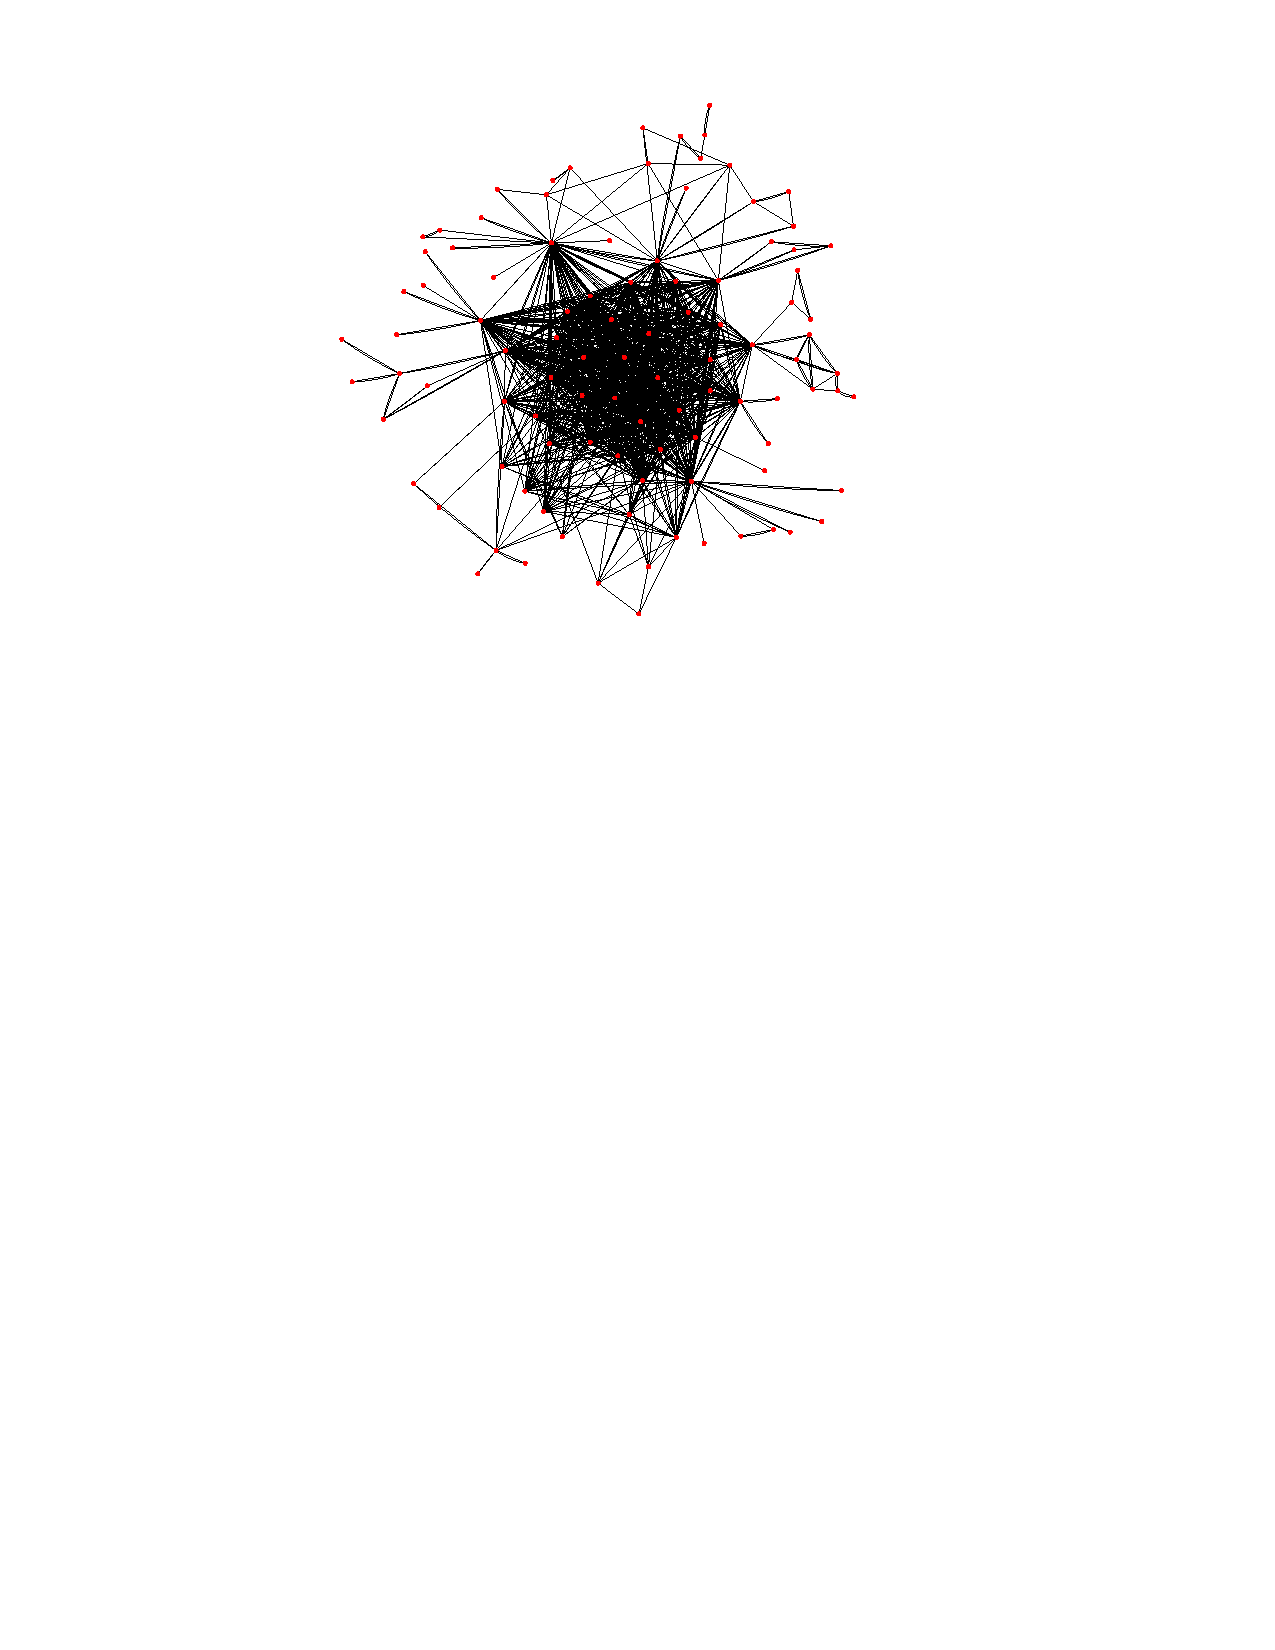
\includegraphics[scale=1.5]{images/subgraph-label-time-fa62cc57cd35e9f90b85435efc407ad5.pdf}
  \caption{Community mit zeitlicher Korrelation der Signaturen
    (Blondel ($l=5$),
    100 Knoten, 72\% der Signaturen innerhalb eines Monats)}
  \label{fig:time-corr-com-normal}
\end{figure}


\begin{figure}[th!]
  \centering
  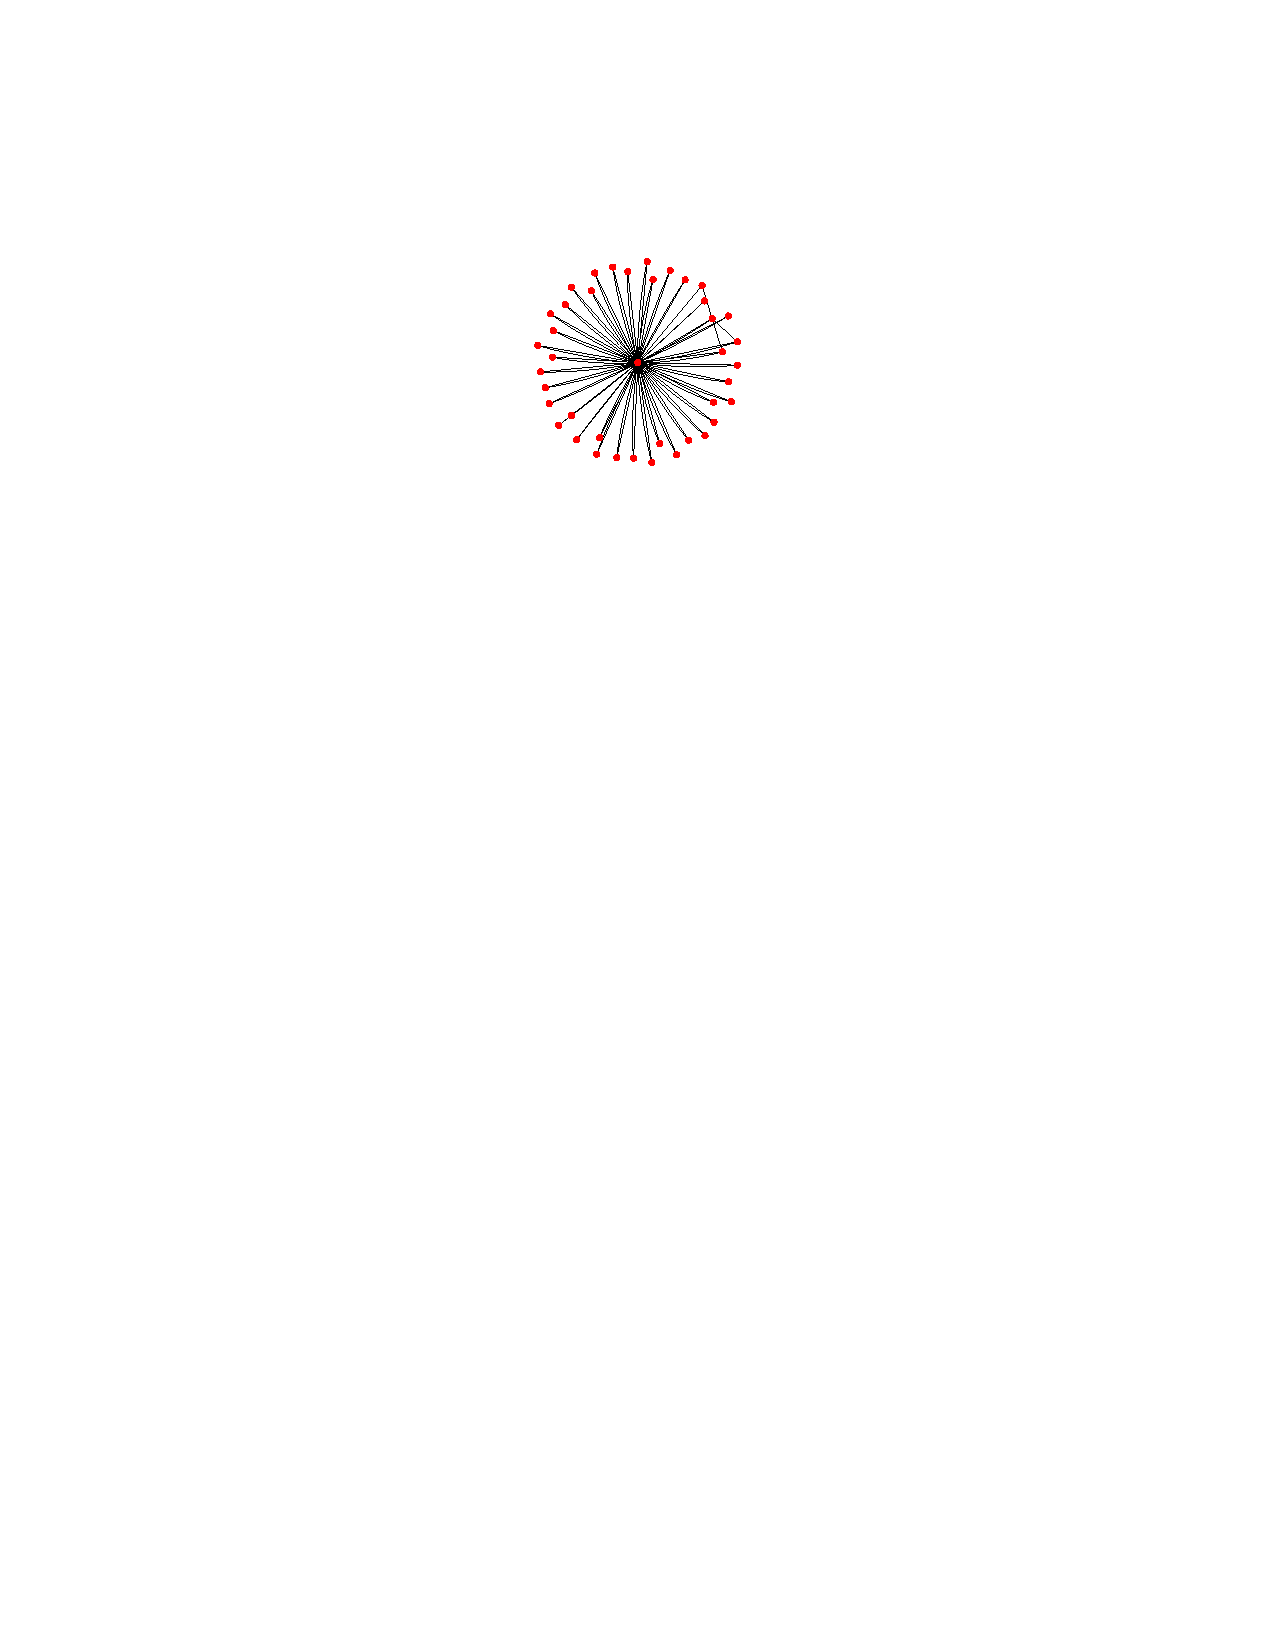
\includegraphics[scale=1.3]{images/label-subgraph-41-star-c222345bc5eb1f9eff80d58a81861974.pdf}
    \caption{Community mit zeitlicher Korrelation der Signaturen
      (Blondel ($l=5$),
      41 Knoten, 84 \% der Signaturen innerhalb eines Monats)}
  \label{fig:time-corr-com-star}
\end{figure}

Es stellt sich die Frage, ob die zeitliche Korrelation der Signaturen
in einer Community ein geeignetes Mittel ist, um Keysigning-Parties zu
erkennen. Neben dem zeitlichen Zusammenhang der Signaturen ist ein
weiteres Merkmal einer Keysigning-Party wie in
Ab. \ref{sec:sozi-komp-des} beschrieben, dass jeder Teilnehmer mit
(fast) jedem anderem Teilnehmer Signaturen austauscht, so dass sich
eine fast vollst\"andige Vermaschung -- fast eine Clique --
ergibt. Eine stichprobenartige Untersuchung in den Communities zeigt,
dass die meisten Communities mit zeitlicher Korrelation zumindest
teilweise dieses Merkmal zeigen. Abbildung
\ref{fig:time-corr-com-normal} zeigt ein Beispiel einer solchen
Community. Etwa die H\"alfte der Knoten ist in einer Fast-Clique
enthalten, deren Knoten mit (fast) allen anderen vernetzt sind. Dieser
innere Teil des Teilgraphen entspricht genau dem Bild, das als
Resultat einer Keysigning-Party erwartet wird. Auch wenn dies auf die
meisten der Communities mit zeitlicher Korrelation zutrifft, gibt es
auch Gegenbeispiele. Abbildung \ref{fig:time-corr-com-star} zeigt eine
Community, die zwar das Kriterium der zeitlichen Korrelation
erf\"ullt, ansonsten aber nichts mit dem erwarteten Bild einer KSP
gemein hat. Allerdings erf\"ullt der Teilgraph trotzdem das Kriterium
der Community, da die Knoten am Rand nur Signaturen zu dem zentralen
Knoten haben und damit die interne Kantendichte deutlich h\"oher ist
als die externe. Um solche Extremf\"alle auszuschliessen, ist als
zus\"atzliches Kriterium f\"ur die Erkennung von KSPs ein hoher
durchschnittlicher Grad der Knoten denkbar.

\begin{figure}[th!]
  \centering
  \subfloat[]{\label{fig:sld-sure-copra1} 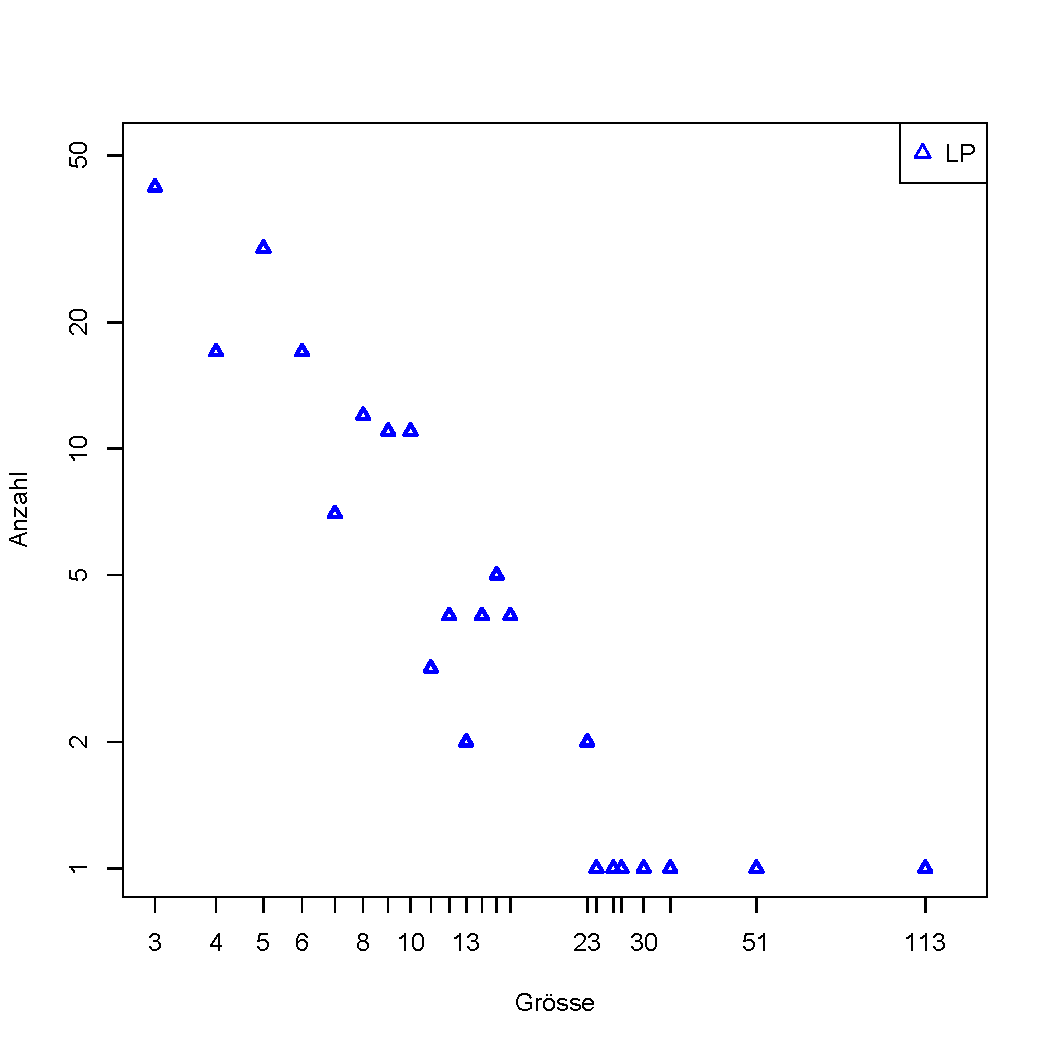
\includegraphics[scale=0.45]{images/sld-sure-ass_copra1.pdf}}
  \subfloat[]{\label{fig:sld-sure-bl2} 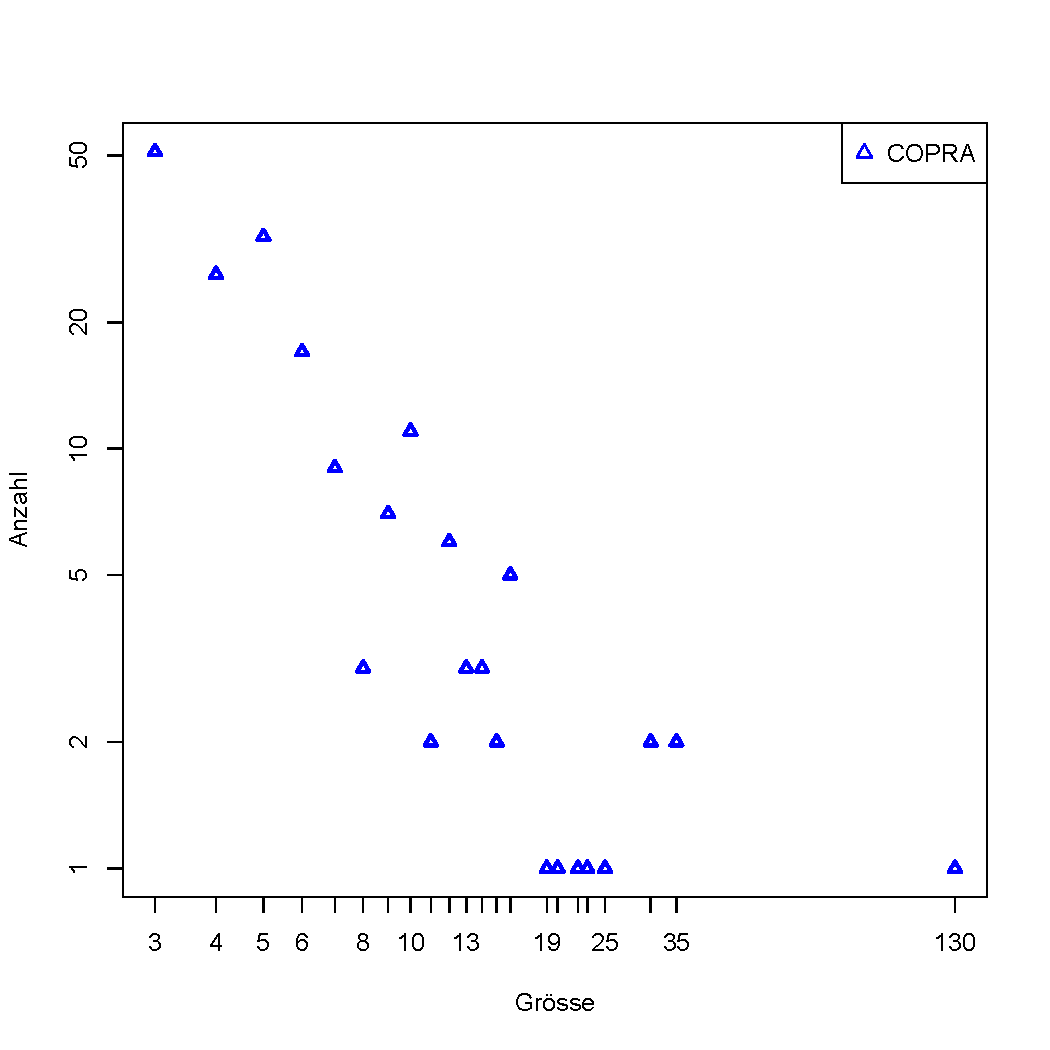
\includegraphics[scale=0.45]{images/sld-sure-ass_copra.pdf}}\\
  \subfloat[]{\label{fig:sld-sure-bl5} 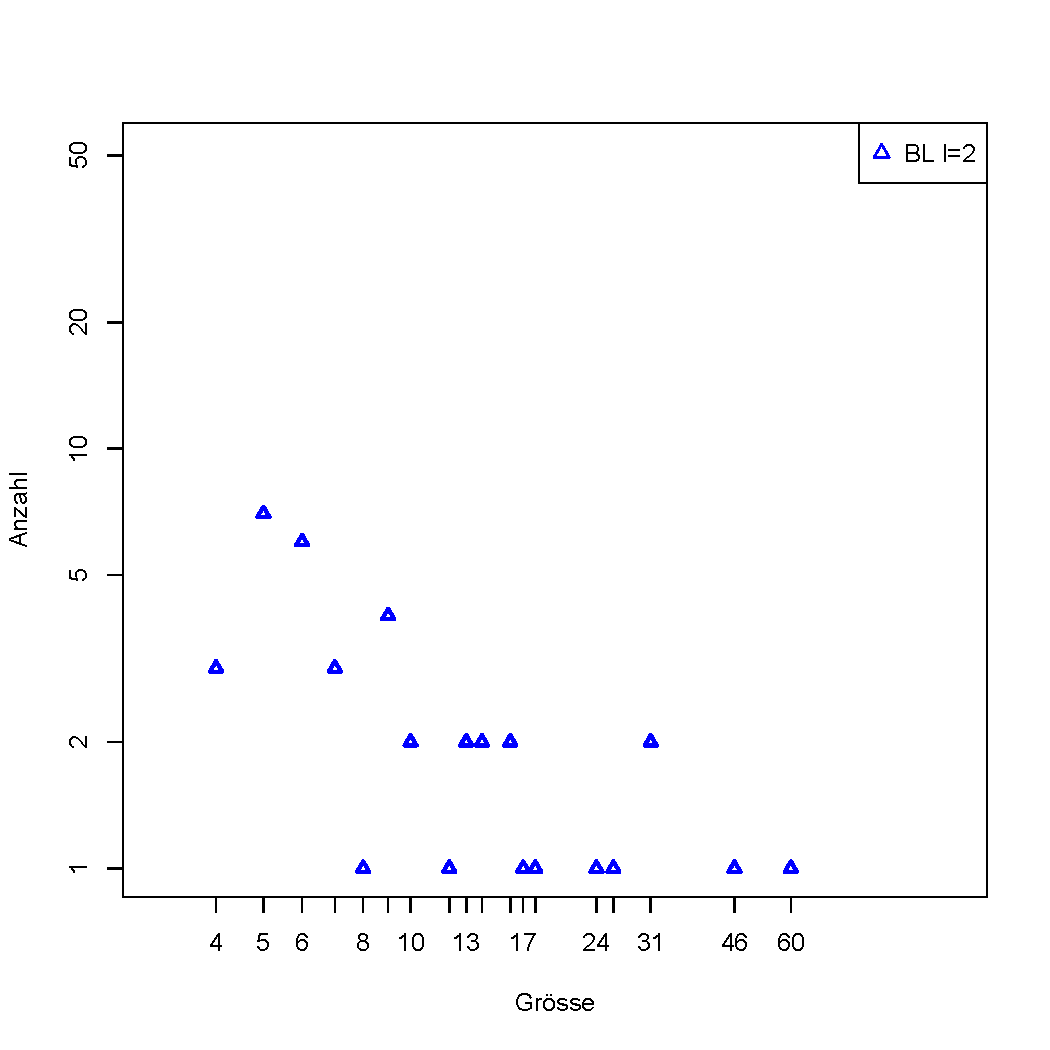
\includegraphics[scale=0.45]{images/sld-sure-ass_bl2.pdf}} 
  \subfloat[]{\label{fig:sld-sure-copra} 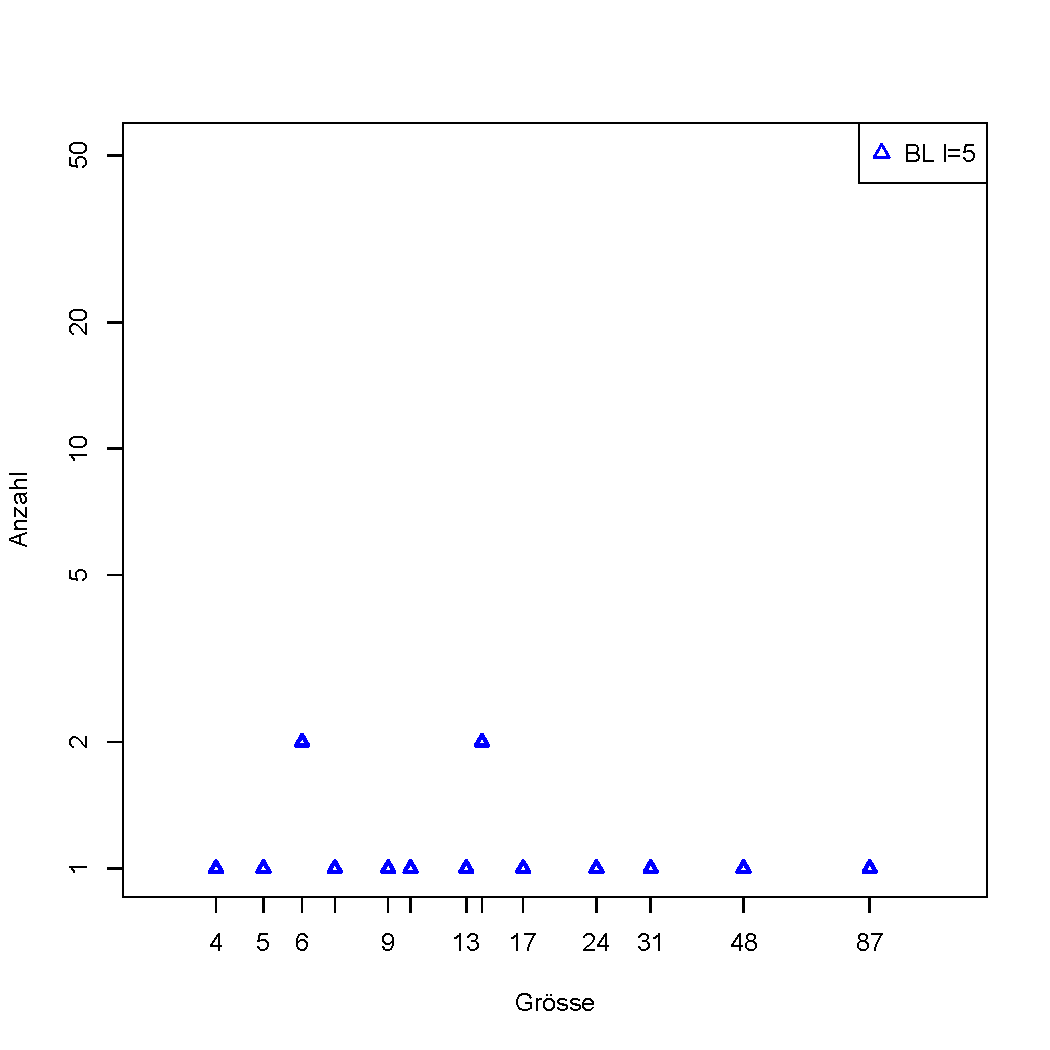
\includegraphics[scale=0.45]{images/sld-sure-ass_bl5.pdf}}
  \caption{Zuweisung von Domains zu SLDs abh\"angig von der Community-Gr\"osse}
  \label{fig:sld-suredist}
\end{figure}

\begin{figure}[th!]
  \centering
  \subfloat[]{\label{fig:sld-maybe-copra1} 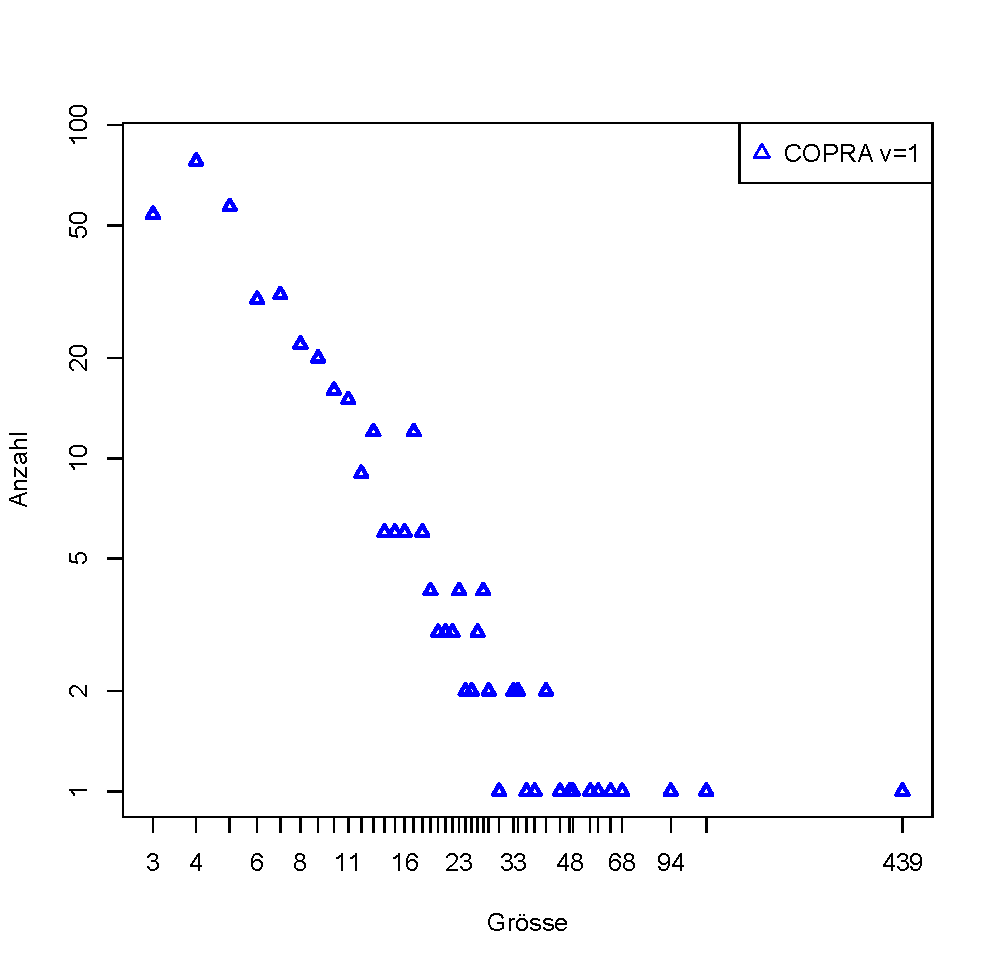
\includegraphics[scale=0.45]{images/sld-maybe-ass_copra1.pdf}}
  \subfloat[]{\label{fig:sld-maybe-bl2} 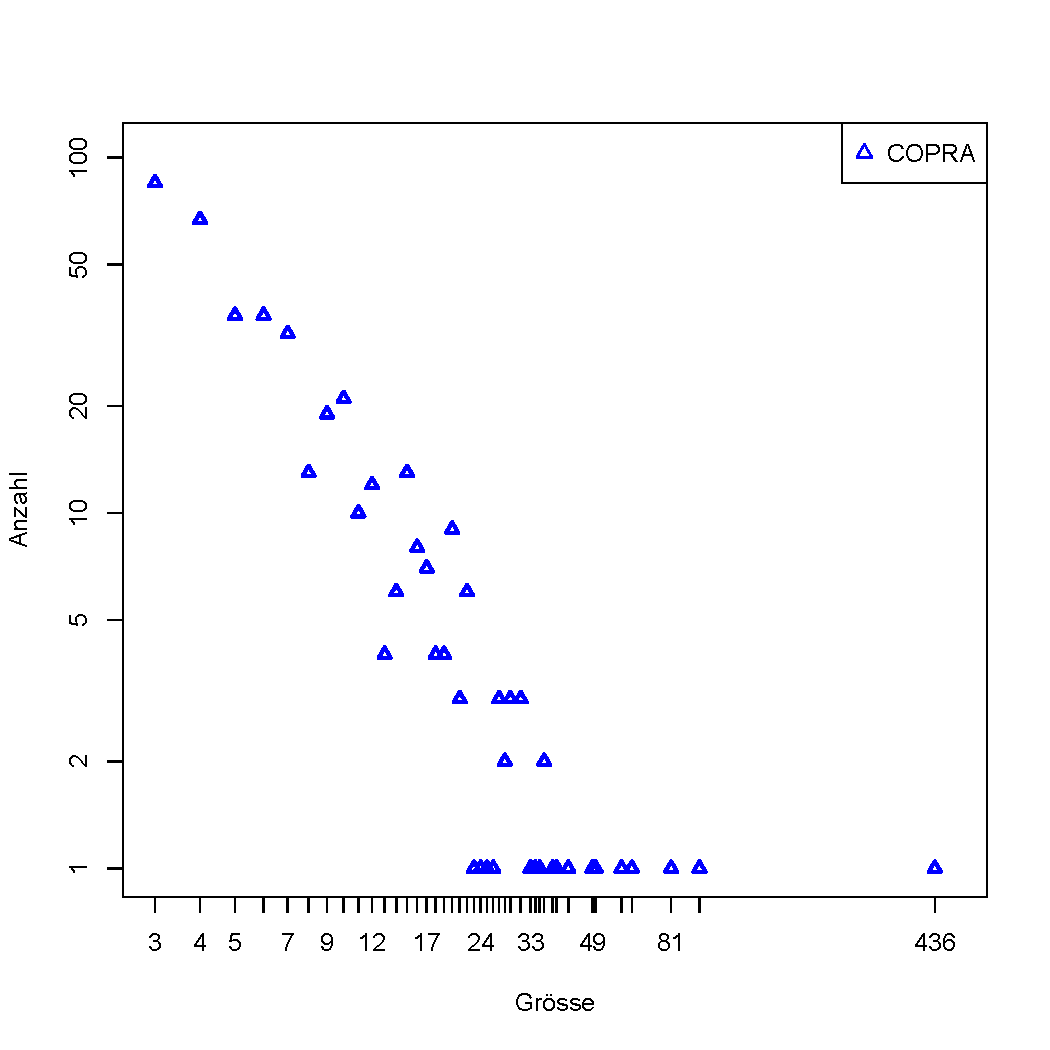
\includegraphics[scale=0.45]{images/sld-maybe-ass_copra.pdf}}\\
  \subfloat[]{\label{fig:sld-maybe-bl5} 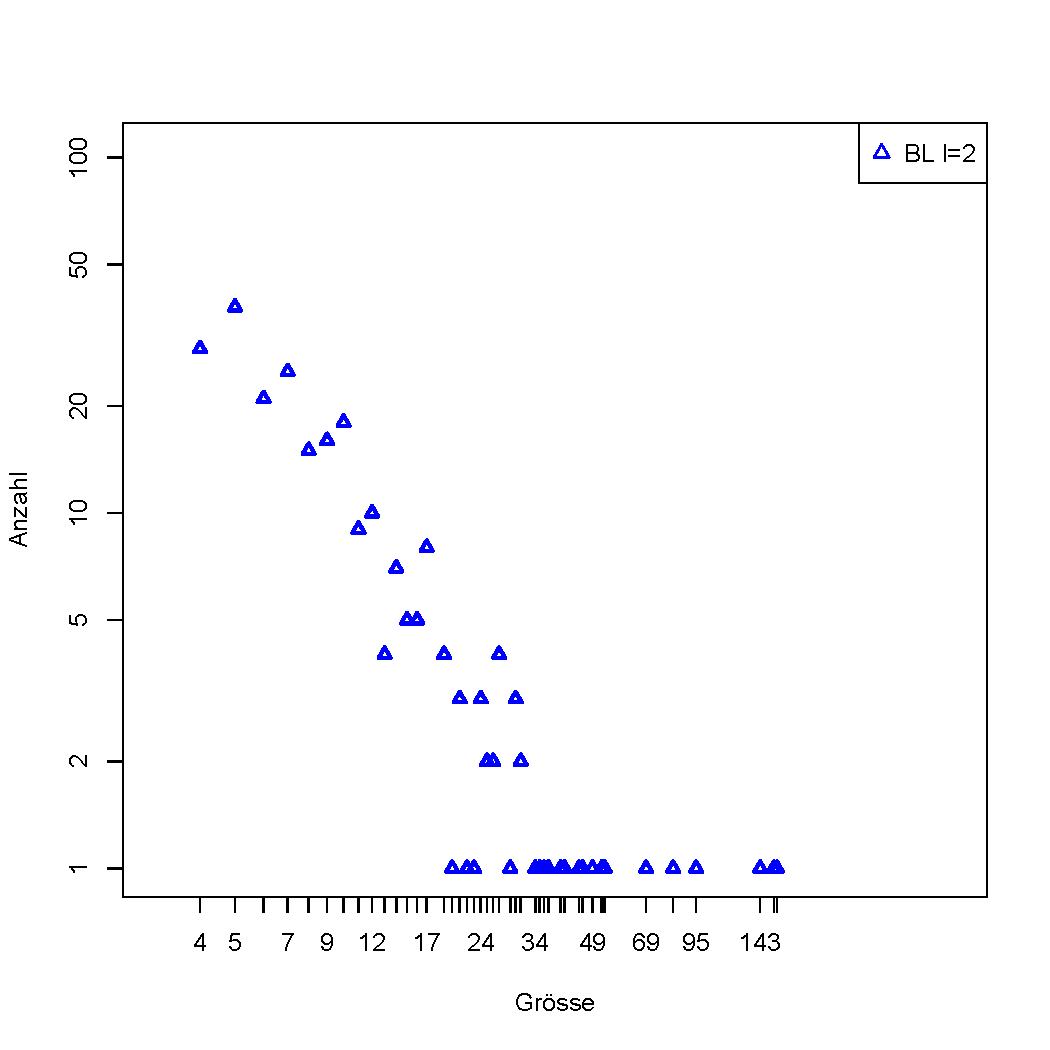
\includegraphics[scale=0.45]{images/sld-maybe-ass_bl2.pdf}} 
  \subfloat[]{\label{fig:sld-maybe-copra} 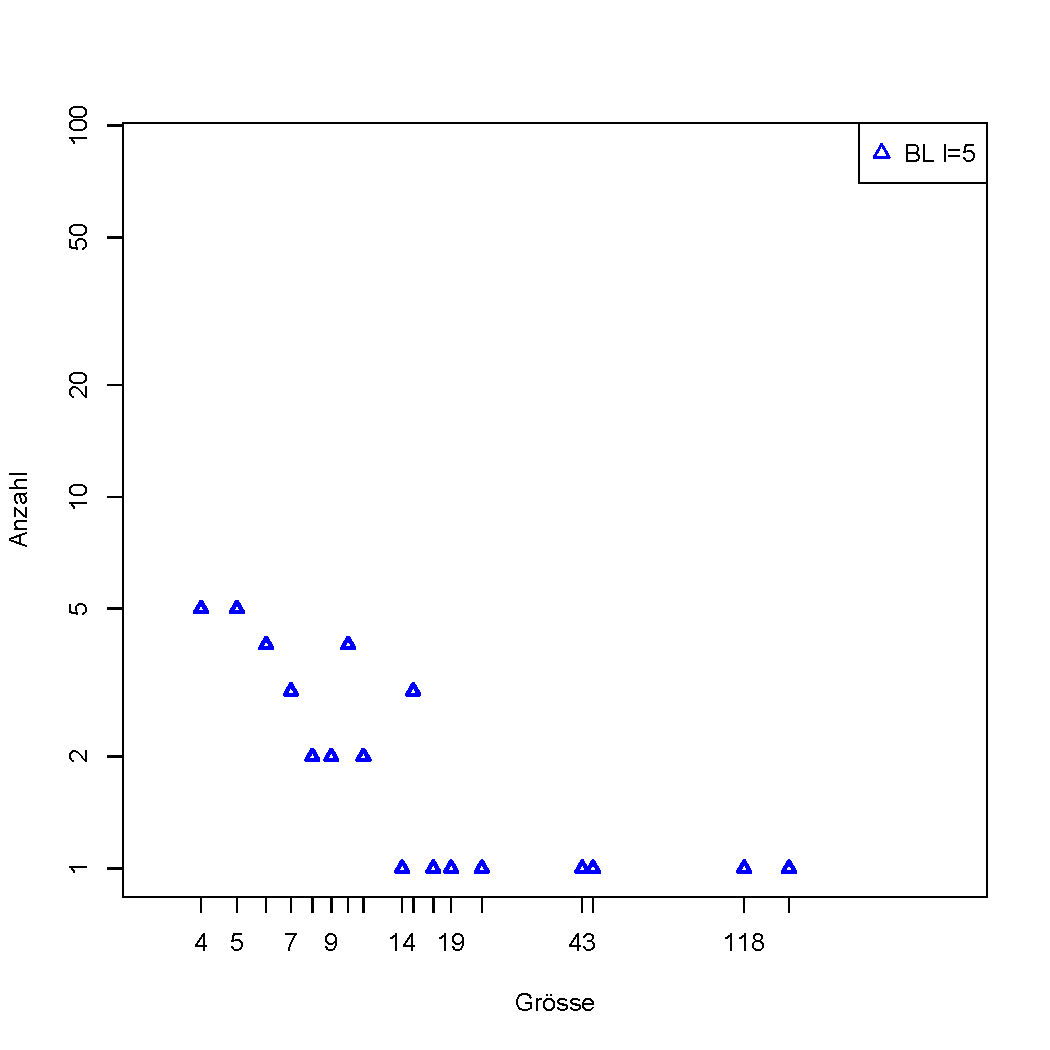
\includegraphics[scale=0.45]{images/sld-maybe-ass_bl5.pdf}}
  \caption{Verteilung der Gr\"osse der von einer SLD dominierten Communities}
  \label{fig:sld-maybedist}
\end{figure}

\begin{figure}[th!]
  \centering
  \subfloat[]{\label{fig:time-corr-copra1} 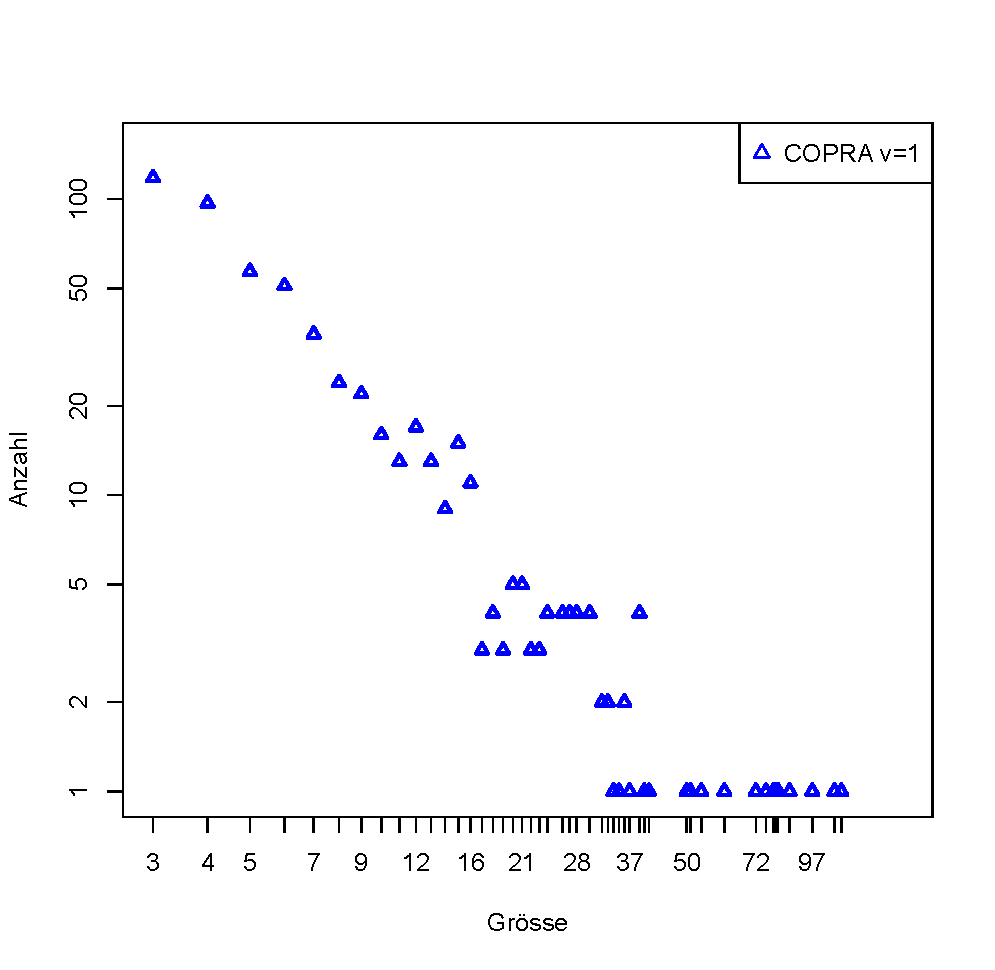
\includegraphics[scale=0.45]{images/time-corr_copra1.pdf}}
  \subfloat[]{\label{fig:time-corr-bl2} 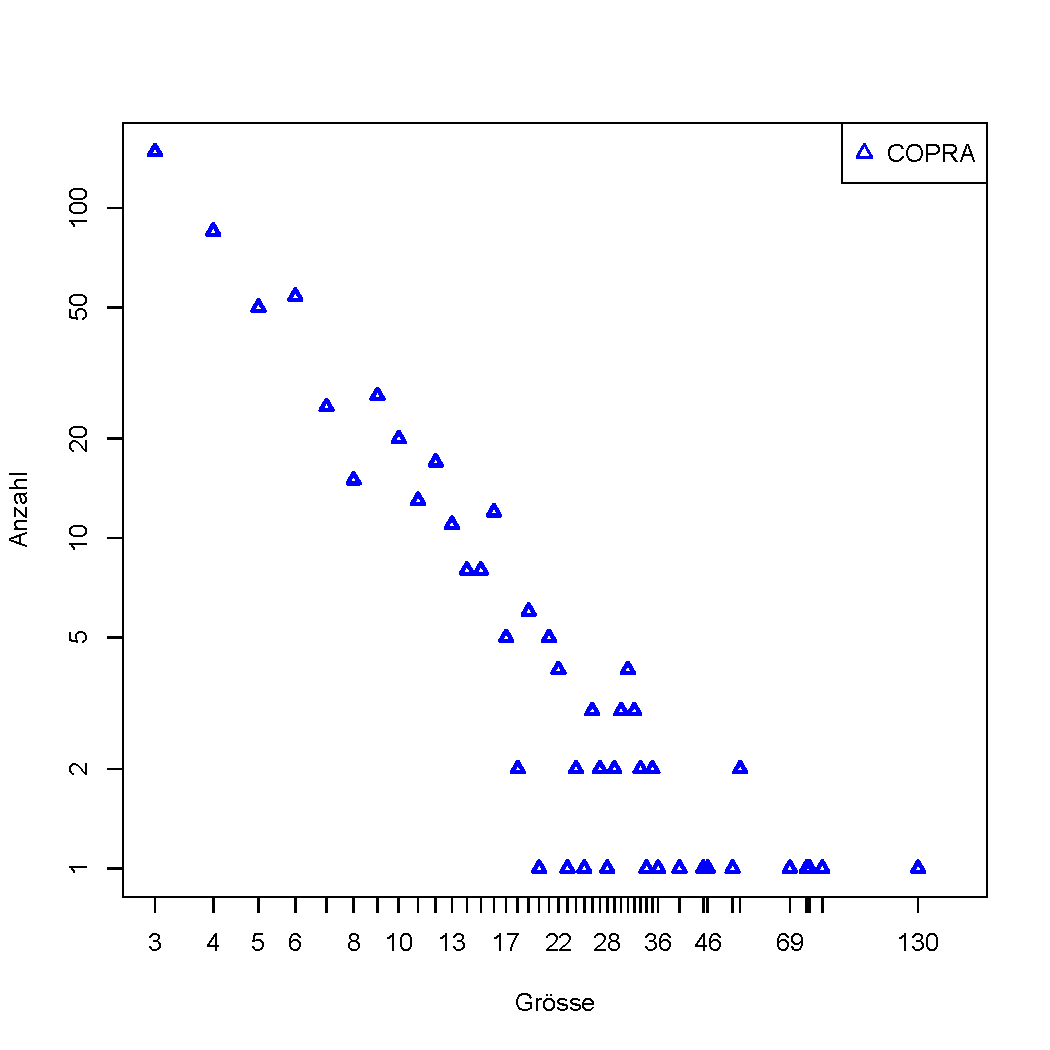
\includegraphics[scale=0.45]{images/time-corr_copra.pdf}}\\
  \subfloat[]{\label{fig:time-corr-bl5} 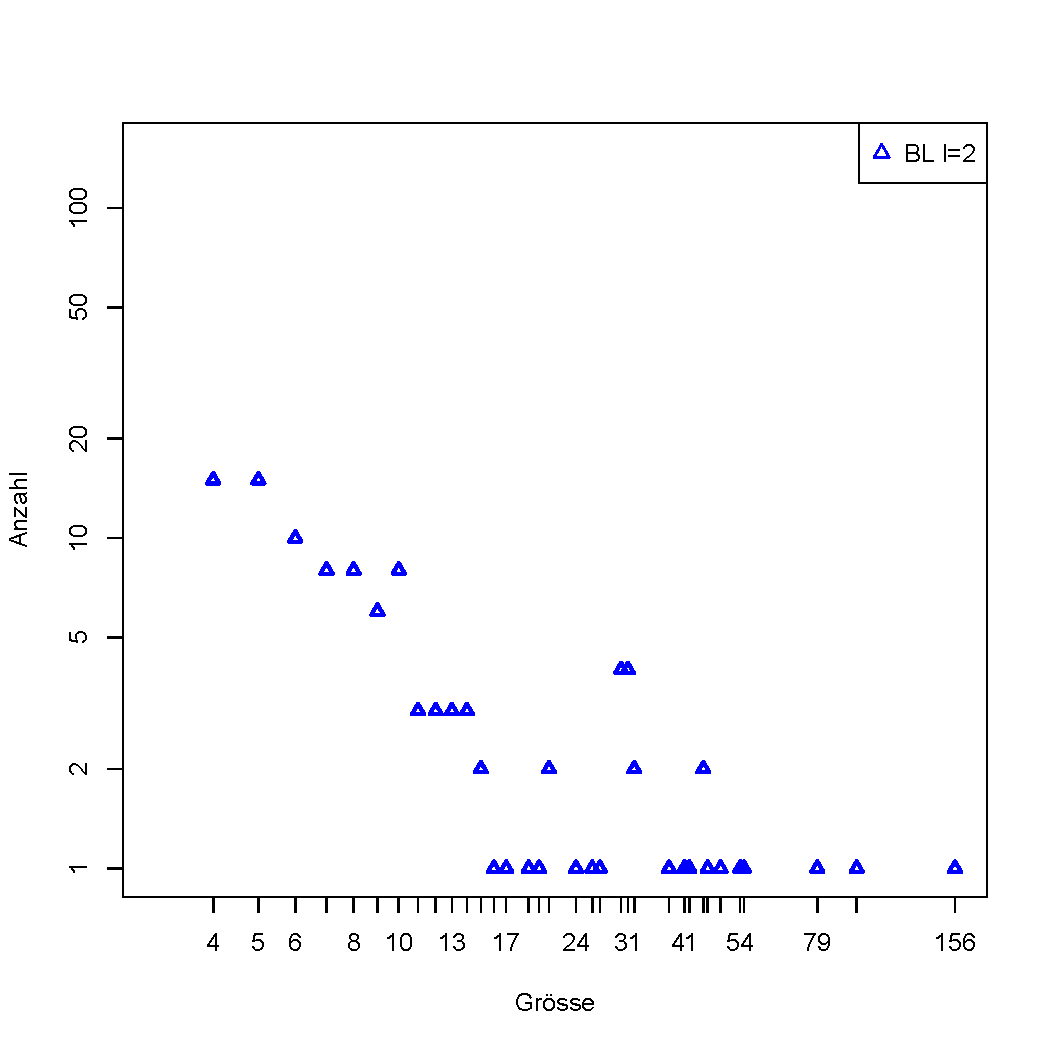
\includegraphics[scale=0.45]{images/time-corr_bl2.pdf}} 
  \subfloat[]{\label{fig:time-corr-copra} 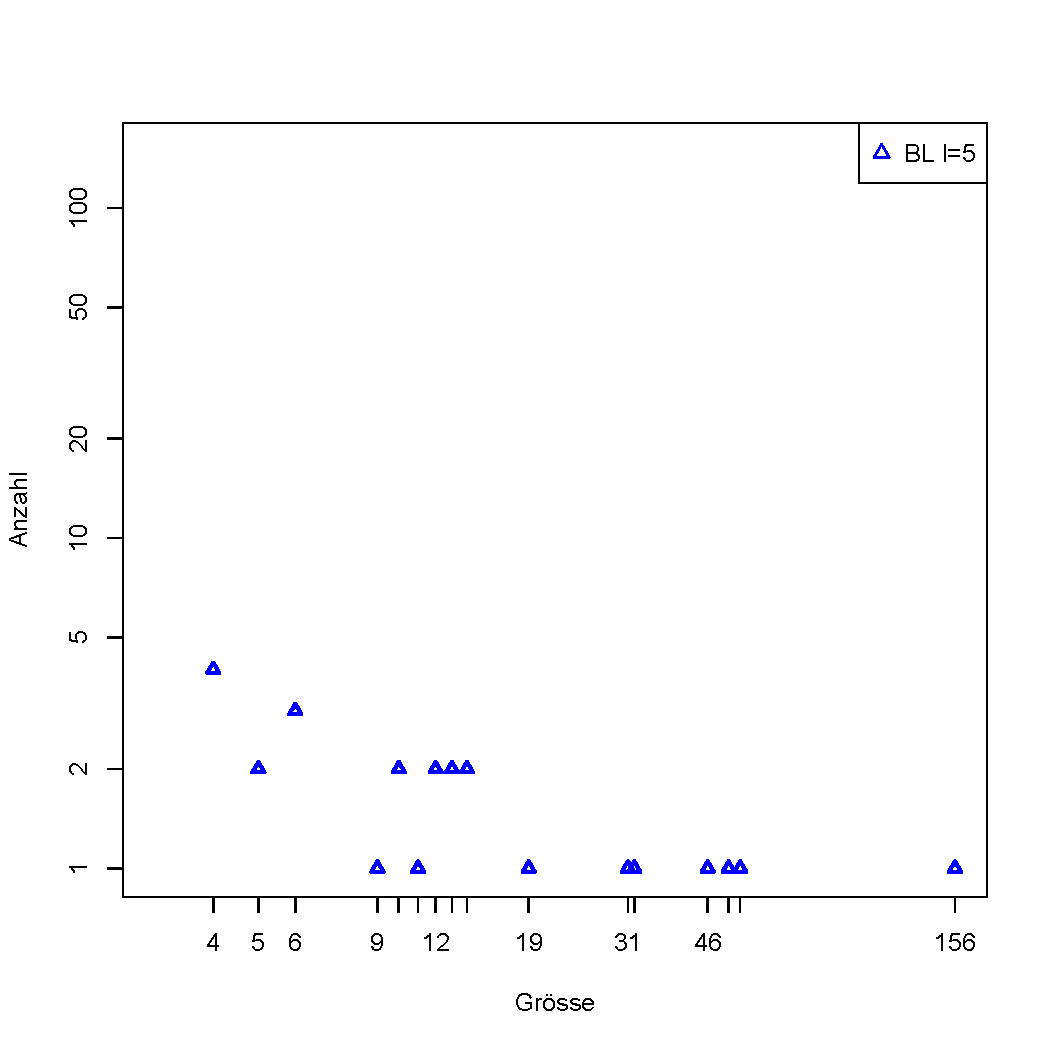
\includegraphics[scale=0.45]{images/time-corr_bl5.pdf}}
  \caption{Verteilung der Gr\"osse von Communities mit zeitlicher
    Korrelation der Signaturen}
  \label{fig:time-corrdist}
\end{figure}

Diese Ergebnisse widerlegen nicht die Annahme, dass die Vernetzung im
Web of Trust im wesentlichen von Keysigning-Parties und den sozialen
Kontakten der Teilnehmer beeinflusst wird und damit unter anderem von
Gruppenzugeh\"origkeit bestimmt wird. Allerdings muss festgehalten
werden, dass die hier verwendeten Methoden nicht geeignet sind, um den
Entstehungsmechanismus entlang dieser Annahme befriedigend zu
erkl\"aren. 

Ein Grund daf\"ur ist sicherlich, dass die Struktur des Web of Trust
nur zu einem bestimmten, festen Zeitpunkt betrachtet wurde. Um die
Entstehungsdynamik zu verstehen, k\"onnte alternativ die Entwicklung
des Netzwerks tats\"achlich \"uber die Zeit nachvollzogen werden. Das
Keyserver-Netzwerk speichert nicht nur den momentanen Zustand des
Netzwerks, sondern implizit auch den Entstehungszeitpunkt jedes
Schl\"ussels und jeder Signatur. Die im Rahmen dieser Arbeit
entwickelte Software speichert diese Zeitstempel in einer Datenbank
und macht so die gesamte Entwicklungsgeschichte des Web of Trust
verf\"ugbar (siehe Abschnitt
\ref{ch:Grundlagen:sec:Design:subsec:eigene-software}). Anhand dieser
Daten k\"onnte nachvollzogen werden, wie und in welcher Form die
Communities tats\"achlich entstehen und sich entwickeln.

Dass nur sehr wenige gr\"ossere Communities mit zeitlicher Korrelation
der Signaturen gefunden wurden, obwohl regelm\"assig gr\"ossere
Keysigning-Parties stattfinden (siehe Abschnitt
\ref{sec:sozi-komp-des}) ist bei n\"ahrerer Betrachtung durchaus
plausibel. Dass eine Keysigning-Party sich in der Struktur markant
abhebt, setzt vorraus, dass ihre Teilnehmer ausser der Teilnahme an
dieser Party keine wesentliche Signaturaktivit\"at starten. W\"urden
sie weiterhin an Signaturaktitiv\"aten teilnehmen, w\"urde die
Struktur der Keysigning-Party mit der Zeit durch Signaturen von und zu
Nicht-Teilnehmern ``verwischt'' werden. Aufgefunden wurden also
vermutlich nur die Keysigning-Parties mit einer Mehrheit von insgesamt
eher inaktiven Teilnehmern. Gleiches kann f\"ur Teilnehmer angenommen
werden, die sich anhand von Gruppenzugeh\"origkeit vernetzen. Auch
hier w\"urde die Struktur mit der Zeit ``unsch\"arfer'' werden, wenn
ihre Mitglieder weiterhin Signierungen vornehmen w\"urden. Es kann
also angenommen werden, dass die kleineren und insbesondere die klar
zuordnenbaren Communities tendenziell Teilnehmer enthalten, die in
Bezug auf die Teilnahme am Web of Trust eher inaktiv sind. Um diese
Vermutung zu best\"atigen oder zu wiederlegen, k\"onnte das
Signaturverhalten der Teilnehmer \"uber die Zeit mit ihrer
Community-Mitgliedschaft verglichen und korreliert werden.

Es scheint unrealistisch, dass die Mitgliedschaft in einer Gruppe --
etwa einer Firma, akademischen Einrichtung oder einem
Open-Source-Projekt -- die sozialen Kontakte einer Person
vollst\"andig charakterisiert. Daneben kann eine Person noch ein
weites Netzwerk an Freunden oder Bekannten haben, die diese
Mitgliedschaft nicht teilen. Trotzdem k\"onnen sich zu ihnen
Signaturen ergeben, die einen wesentlichen Teil der Signaturen dieser
Person ausmachen k\"onnen. Ausserdem ist anzunehmen, dass eine
Vielzahl solcher Gruppen nicht \"uber eine gemeinsame Domain
verf\"ugen, und damit mit den hier vorliegenden Daten schlicht nicht
sichtbar sind. Zwar wurde versucht, der anzunehmenden Komplexit\"at
der Gruppenzugeh\"origkeiten durch \"uberlappende Communities zu
begegnen. Allerdings konnte der verwendete Algorithmus keine
signifikanten \"Uberlappungseigenschaften liefern . Die Frage,
inwiefern sich die einzelnen Communities sozialen Gruppen zuordnen
lassen, konnte also nur unvollst\"andig beantwortet werden.

Es zeigt sich, dass dem Web of Trust kein einzelner, einfacher
Entstehungsmechanismus der hier angenommenen Form zugrundeliegt. Es
kann nur unzureichend beschrieben werden als eine Ansammlung von
einzelnen, einfach entstandenen Bausteinen, als die hier Communities
angenommen wurden. Implizit vorrausgesetzt wird dabei auch, dass diese
zum Beispiel im Fall einer Keysigning-Party nach ihrer Entstehung
keine wesentliche weitere Vernetzungsaktitiv\"at zeigen. Zwar trifft
dies f\"ur einen Teil der Communities -- gerade die, die eine
zeitliche Korrelation der Signaturen zeigen oder einer
Second-Level-Domain zugeordnet werden k\"onnen -- durchaus zu. F\"ur
einen erheblichen Anteil der Teilnehmer -- beispielsweise die
Mitglieder der sehr grossen Community aus der COPRA-Berechnung --
scheint die Vernetzung jedoch so vielf\"altig zu sein, dass solche
einfachen Mechanismen nicht mehr sichtbar sind und ``in der Masse
verschwinden''. Bei der COPRA-Zerlegung ist es etwa naheliegend, dass
die sehr grosse zentrale Community die Mehrzahl der aktiveren
Teilnehmer enth\"alt. Hier ergibt sich eine \"Ahnlichkeit zur Struktur
der Zusammenhangskomponenten, bei denen die gr\"osste alle aktiven
einigermassen aktiven Teilnehmer zu enthalten scheint (siehe Abschnitt
\ref{sec:result-komponentenstruktur}).

Diese Punkte k\"onnen anhand des Beispiels von Debian illustriert
werden: Das Debian-Projekt als tats\"achliche Community, in der
PGP und das Web of Trust eine besonders wichtige Rolle spielen (siehe
Abschnitt \ref{sec:sozi-komp-des}) findet sich in den Zerlegungen
nicht als eigene abgregrenzte Einheit wieder. Statt dessen finden sich
sehr grosse Communities, in denen Debian-Entwickler einen signifikaten
Anteil der Schl\"ussel stellen. Im Fall der COPRA-Zerlegung ist dies
die bereits erw\"ahnte Community mit ca. 21000 Mitgliedern. Von diesen
verf\"ugen 1247 \"uber eine E-Mail-Adresse in der Domain debian.org
und sind damit offensichtlich Mitglieder des Debian-Projekts. Daneben
finden sich Mitglieder des Debian-Projekts in einer Vielzahl von
kleineren Communities aller Gr\"ossen. Die Mitgliedschaft im
Debian-Projekt scheint hier also f\"ur die Vernetzung keine so
wesentliche Rolle zu spielen, dass sie die Struktur dieser real
existierenden Community im Web of Trust wiederspiegelt. Selbst wenn viele
Debian-Entwickler mit vielen anderen Projektmitgliedern vernetzt sind,
so verf\"ugen sie offensichtlich \"uber gen\"ugend andere Kontakte,
so dass diese Struktur nicht mehr auffindbar ist.

%%% Local Variables: 
%%% mode: latex
%%% TeX-master: "diplarb"
%%% End: 

